\documentclass[a4paper,12pt,times,numbered,print,index]{report}
\usepackage[english]{babel}
\usepackage[utf8]{inputenc}

\oddsidemargin  0.01mm       % USA 5mm?
\evensidemargin 0.01mm       % USA 5mm?
\headheight -0.03mm             % 10mm ok
\headsep  -0.03mm
\hoffset -3mm
           % was commented out before
\textheight 250mm            % USA 240mm?
\textwidth 180mm             % USA 160mm?
\topmargin -10mm           % before 18/5/93 this was -20mm
\topskip -10mm

\renewcommand{\baselinestretch}{1.5}

\renewcommand {\arraystretch}{1.0}


\usepackage{dcolumn}
\usepackage{amsmath}
\usepackage{amssymb}
\usepackage{graphicx}
\usepackage{pdfpages}
\usepackage{fullpage}
\usepackage{caption}
\usepackage{float}
\usepackage{fancyhdr}
\usepackage{amsmath}
\usepackage{multirow}
\usepackage{commath}
\usepackage{natbib}
\setcitestyle{aysep={,}}
%\usepackage{apacite}
%\usepackage{biblatex}
\usepackage{mathtools}
\usepackage{subcaption}
\usepackage{mathrsfs,amssymb}
\usepackage{amsthm}
\usepackage{enumitem}
\usepackage{booktabs}
\usepackage{verbatim}
\usepackage{enumitem,kantlipsum}
\usepackage{chngcntr}
\usepackage{apptools}
\usepackage{adjustbox}
\usepackage{epstopdf}
\usepackage{pdflscape}
\usepackage{afterpage}
\usepackage[pdftex,colorlinks=true,linkcolor=cyan,linktoc=all]{hyperref}
\usepackage{siunitx}
\usepackage{authblk}
\usepackage{soul}

\usepackage{titletoc}% http://ctan.org/pkg/titletoc
\titlecontents*{chapter}% <section-type>
[0pt]% <left>
{}% <above-code>
{\bfseries\chaptername\ \thecontentslabel\quad}% <numbered-entry-format>
{}% <numberless-entry-format>
{\bfseries\hfill\contentspage}% <filler-page-format>


\usepackage[font=footnotesize,labelfont=bf]{caption}
\captionsetup[sub]{font=scriptsize,labelfont=bf}
%\newcommand*{\fullref}[1]{\hyperref[{#1}]{\autoref*{#1} \nameref*{#1}}}

\renewcommand{\sectionautorefname}{Section}
\renewcommand{\subsectionautorefname}{Section}
\renewcommand\thesection{\arabic{section}}

\interfootnotelinepenalty=10000
\setcitestyle{aysep={,}}
\newcolumntype{L}{@{}l@{}}
\newcommand{\mc}[1]{\multicolumn{1}{c}{#1}}
\sisetup{table-space-text-post = **}
\definecolor{darkblue}{rgb}{0,0,.6}
\hypersetup{citecolor=darkblue,linkcolor=darkblue,urlcolor=darkblue}



%\mathchardef\colon="603A
%\appendix{\counterwithin{lemma}{section}}


\makeatletter
%% The "\@seccntformat" command is an auxiliary command
%% (see pp. 26f. of 'The LaTeX Companion,' 2nd. ed.)
\def\@seccntformat#1{\@ifundefined{#1@cntformat}%
   {\csname the#1\endcsname\quad}  % default
   {\csname #1@cntformat\endcsname}% enable individual control
}
\let\oldappendix\appendix %% save current definition of \appendix
\renewcommand\appendix{%
    \oldappendix
    \newcommand{\section@cntformat}{\appendixname~\thesection\quad}
}
\makeatother
\usepackage{cleveref} % just for this example



%\renewcommand{\&}{and}
\numberwithin{equation}{section}
\newtheorem{theorem}{Theorem}[section]
\DeclareMathOperator*{\argmin}{argmin}
\newtheorem{remark}{Remark}[section]
\newtheorem{assumption}{Assumption}
\allowdisplaybreaks
\newtheorem{lemma}{Lemma}

\newcommand{\assumptionautorefname}{Assumption}
\newcommand{\lemmaautorefname}{Lemma}
\newcommand{\qedd}{\tag*{$\qed$}}


\pagestyle{fancy}
\fancyhf{}
\renewcommand{\headrulewidth}{0pt}
%\renewcommand{\headrulewidth}{0.1pt} % for upper line
%\rhead{Weilun Zhou}
%\lhead{Confirmation Report}
\cfoot{\thepage}
%\setlength{\headsep}{0.3in}

%=============================
\begin{document}

% \begin{titlepage}
% 	\begin{center}
% 		\vspace*{1cm}
		
% 		\Huge
% 		\textbf{Partially Nonlinear Single-Index Models}
		
% 		\vspace{2.5cm}
		
% 		\large
% 		\textbf{Ying Zhou} \\
		
% 		\vspace{0.5cm}
		
% 		Supervised by: \\
% 		Professor Jiti Gao \\
% 		Dr Hsein Kew
		
% 		\vfill
		
% 		A thesis presented for PhD progress review.
		
% 		\vspace{0.8cm}
		
% 		
\includegraphics[width=0.4\textwidth]{monash-university-logo.png}
		
% 		Department of Econometrics and Business Statistics \\
%		Monash University\\

% 		March,  2021
		
% 	\end{center}
% \end{titlepage}

\pagenumbering{arabic}

\chapter*{Chapter 3: Partially Nonlinear Single-Index Predictive Model}

\section{Introduction}
%Partial-linear model is an important tool for multivariate regression due to its flexibility. It combines linear model with a nonparametric model, which can capture both linear and nonlinear relationship between dependent variable and predictors (see for example \cite{stute2005nonparametric}). Such works include Such works include \cite{chen1988convergence}, \cite{carroll1997generalized} and \cite{ruppert2003semiparametric}. Due to the "curse of dimensionality", the nonlinear relationship in the nonparametric part can be difficult to explore (see for example, \cite{ma2013doubly}). Therefore, we follow \cite{dong2016estimation} and consider a partial linear single-index model of the form:

Conventional partially linear models involving both parametric and nonparametric components have been widely studied in the literature, such as by \cite{gao2007nonlinear}. In the time series literature, partially linear single-index models have also attracted attention in recent years, see for example \cite{dong2016estimation}. We are now interested in a new class of nonlinear time series models - partially nonlinear single-index models of the form:
\begin{equation}
y_{t} = \beta_0^{\prime} z_t + f\left( x_{t-1}^{\prime }\theta_0; \gamma_0\right) +e_{t},\ \ \
t=2,...,T,  \label{PL model}
\end{equation}%
where $z_t = (y_{t-1}, \cdots, y_{t-p}, w_{t-1}^{\prime})^{\prime}$, in which $w_{t-1}$ is a vector of stationary predictors, 
%such as the 3 components (consumption, labour income and asset holdings) of "cay" variable constructed by \textcolor[rgb]{ 0,  .439,  .753}{Lettau and Ludvigson (2001)}.
$g\left( .,.\right) $ is a known univariate nonlinear function, $x_{t-1}$ is a $d$-dimensional integrated process of order one, $\theta _{0}$ is a $d$-dimensional unknown true parameter vector that lies in the parameter set $\Theta $, $\gamma _{0}$ is a $m$-dimensional unknown true parameter vector that lies in the parameter set $\Gamma $ and $e_{t}$ is a martingale
difference process. The parameter sets $\Theta $ and $\Gamma $ are assumed to be compact and convex subsets of $\mathbb{R}^{d}$ and $\mathbb{R}^{m}$ respectively. In order to ensure that $\theta_0$ is uniquely identifiable, we will need to impose $\theta_{0}^{\prime}\theta_{0} = 1$.

Our model allows for lagged dependent variables because key macroeconomic/financial variables, such as the growth rate of GDP, the rate of unemployment and interest rates are typically autocorrelated. Failing to account for this autocorrelation will lead to serially correlated residuals. We are thus interested in using this model to assess whether including lagged dependent variables would, in fact, improve forecasts of $y_{t}$ relative to using only the nonlinear single-index component, $f\left( x_{t-1}^{\prime }\theta_0; \gamma_0\right)$, containing either the cointegrated predictors or non-cointegrated predictors. Our model may also be useful in cases where there are additional stationary predictors, $w_{t-1}$, for which the linear specification fits the data better than the nonlinear specification.

There is a considerable theoretical effort being put into developing new estimation method of the partial linear model (see for example, \cite{dong2016estimation}) and nonlinear models with single-index (see for example \cite{chang2003index}). In our study, we propose a novel 2-step estimation method in which $\beta$ will have a closed form solution while $\theta$ and $\gamma$ can be estimated by the method of nonlinear least squares or constrained nonlinear least squares.

This study aims to use the Monte Carlo simulation method to investigate the finite sample properties of the estimators. There will also be an empirical analysis to study the predictability of stock returns. We will use the dataset from \cite{welch2008comprehensive} and investigate the out-of-sample forecast ability of model (\ref{PL model}). Compared with chapter 2, we will include lagged dependent variables in the model. We will investigate whether the partially nonlinear single-index model will help further improve the stock return predictability in my future research.  

This chapter is organized as follows. Section 2 introduces the partially nonlinear single-index predictive model and proposes a 3-step estimation method. To improve the performance of the model, this section also introduces constraint and truncation conditions in addition to the normal nonlinear least square. Section 3 examines the finite-sample properties of the normal nonlinear least square estimators (NLS estimators hereafter) and the constrained nonlinear least square estimators (CLS estimators hereafter) using Monte Carlo evaluation. The discussion includes models with different nonlinear functional part and considers both co-integrated and non-cointegrated cases. Section 4 applies the partially nonlinear models to stock return predictability and investigate both in-sample and out-of-sample performances of the models. Section 5 concludes. 

%One of the motivation of considering this model is the different time series properties in predictors  
%
%Model \ref{PL model} considered both stationary and nonstationary time series, especially that the lagged dependent variables have been included in the linear component. In this chapter, we will extend 
\section{Model and Methodology}
\subsection{Estimation Method}
Since in our case, $f\left( x_{t-1}^{\prime }\theta_0; \gamma_0\right)$ is known, model (\ref{PL model}) can be estimated by using a nonlinear least square method. Let $L(\beta, \theta, \gamma) = \sum_{t=1}^{T} \left( y_t - \beta^{\prime} z_t - f\left( x_{t-1}^{\prime }\theta; \gamma\right)\right) ^2$, and hence we have the following gradient functions:


\begin{align}
	\begin{split}
	\frac{\partial L(\beta, \theta, \gamma)}{\partial \beta} &= -2\sum_{t=1}^{T} z_t^{\prime} \left( y_t - \beta^{\prime} z_t - f\left( x_{t-1}^{\prime }\theta; \gamma\right)\right) \\
	\frac{\partial L(\beta, \theta, \gamma)}{\partial \theta} &= -2\sum_{t=1}^{T} \left( y_t - \beta^{\prime} z_t - f\left( x_{t-1}^{\prime }\theta; \gamma\right)\right)\frac{\partial g(x_{t-1}^{\prime }\theta; \gamma)}{\partial \theta} \\
	\frac{\partial L(\beta, \theta, \gamma)}{\partial \gamma} &= -2\sum_{t=1}^{T} \left( y_t - \beta^{\prime} z_t - f\left( x_{t-1}^{\prime }\theta; \gamma\right)\right) \frac{\partial g(x_{t-1}^{\prime }\theta; \gamma)}{\partial \gamma}
	\end{split}
	\label{gradient}
\end{align}


The minimum value of $L(\beta, \theta, \gamma)$ occurs when the above gradient functions equals to 0. Notice that these score functions $\frac{\partial L(\beta, \theta, \gamma)}{\partial \theta}$ and $\frac{\partial L(\beta, \theta, \gamma)}{\partial \gamma}$ are nonlinear functions of both the variables and the parameters, and so they do not have closed form solutions. To estimate the parameters, we need to include an iterative procedure and obtain optimal values by using gradient descent algorithms. However, recognising that this score function $\frac{\partial L(\beta, \theta, \gamma)}{\partial \beta}$ is linear in the parameter $\beta$, we introduce a novel two-step approach for estimation in order to reduce the computational burden. 

\textbf{Step 1:} set $\frac{\partial L(\beta, \theta, \gamma)}{\partial \beta} = 0$ and solve the first equation in \ref{gradient} to obtain $\tilde{\beta}$:
\begin{equation}
\tilde{\beta} = \left( \sum_{t=1}^{T}z_t z_t^{\prime}\right)^{-1}\sum_{t=1}^{T}\left( y_t - f\left( x_{t-1}^{\prime }\theta; \gamma\right)\right) z_t
\label{beta}
\end{equation}

In other words, $\tilde{\beta}$ is of a linear from by OLS expression. Thus model (\ref{PL model}) can be approximated by:
$$
y_t = \tilde{\beta}^{\prime} z_t + f\left( x_{t-1}^{\prime }\theta; \gamma\right) +e_{t},
$$
Substitute $\bar{\beta}$ in (\ref{beta}) and rearrange the equation above, we can get:
$$
y_t - \left( \left( \sum_{t=1}^{T}z_t z_t^{\prime}\right)^{-1} \sum_{t=1}^{T}y_t z_t \right) ^{\prime} z_t = f\left( x_{t-1}^{\prime }\theta; \gamma\right) - z_t^{\prime} \left( \sum_{t=1}^{T}z_t z_t^{\prime}\right)^{-1} \sum_{t=1}^{T} f\left( x_{t-1}^{\prime }\theta; \gamma\right) z_t + e_t.
$$

Let  
$$\tilde{y} = y_t -  z_t^{\prime}  \left( \sum_{t=1}^{T}z_t z_t^{\prime}\right)^{-1} \sum_{t=1}^{T}y_t z_t, $$ 

$$\tilde{g} ( x_{t-1}^{\prime }\theta; \gamma) = f\left( x_{t-1}^{\prime }\theta; \gamma\right) - z_t^{\prime} \left( \sum_{t=1}^{T}z_t z_t^{\prime}\right)^{-1} \sum_{t=1}^{T} f\left( x_{t-1}^{\prime }\theta; \gamma\right) z_t$$ 
Then we have an approximate model of the form:
\begin{equation}
\tilde{y} = \tilde{g}\left( x_{t-1}^{\prime }\theta; \gamma\right) + e_t.
\label{trans_model}
\end{equation}

\textbf{Step 2: } estimate $(\theta, \gamma)$ using nonlinear least square(NLS) method:
$$
Q_{T}(\theta, \gamma)=\sum_{t=1}^{T}\left(\tilde{y_{t}}-\tilde{g}\left(x_{t-1}^{\prime} \theta, \gamma\right)\right)^{2}
$$
over $(\theta, \gamma) \in (\Theta, \Gamma)$.
The $(\hat{\theta}, \hat{\gamma})$ is given by:
\begin{equation*}
\left( \widehat{\theta},\widehat{\gamma}\right) =\arg \min_{\theta \in \Theta
	,\gamma \in \Gamma }Q_{T}\left( \theta ,\gamma \right),  \label{nls_c3}
\end{equation*}%
which can be solved using an iterative procedure since there is no closed form solution. As $\hat{\theta}$ and $\hat{\gamma}$ have been estimated, we can substitute them back to (\ref{beta}) and get the estimate of $\beta$:
$$
 \hat{\beta} = \left( \sum_{t=1}^{T}z_t z_t^{\prime}\right)^{-1}\sum_{t=1}^{T}\left( y_t- f\left( x_{t-1}^{\prime }\hat{\theta}; \hat{\gamma}\right)\right) z_t.
$$.

In the 2-step procedure above, we have obtained the NLS estimators ($\widehat{\theta}, \widehat{\gamma}, \widehat{\beta}$). In order to improve finite sample properties of the estimators, we impose a truncation condition $I\left(\left\|x_{t-1}\right\| \leq M_T\right)$ on $x_{t-1}$ and an identification condition on coefficient vector $\theta$. We then define the modified sum-of-squared errors by:

$$
Q_{T, M}(\theta, \gamma)=\sum_{t=1}^{T}\left(y_{t}-f\left(x_{t-1}^{\prime} \theta, \gamma\right)\right)^{2} I\left(\left\|x_{t-1}\right\| \leq M_{T}\right)+\lambda\left(\|\theta\|^{2}-1\right),
$$
where $I\left( .\right) $ denotes the indicator function, $%
\left\Vert .\right\Vert $ is the Euclidean norm, $M_T$ is a positive and increasing sequence satisfying $ M_{T}\rightarrow \infty $ as $T \rightarrow \infty $ and $\lambda $ is a Lagrange
multiplier. 

Then in step 1, we can estimate the constrained least squares (denoted CLS) estimators $\bar{\theta}$ and $%
\bar{\gamma}$ by minimizing $Q_{T,M}\left( \theta ,\gamma \right) 
$ over $\theta \in \Theta $ and $\gamma \in \Gamma $ such that the
restriction $\left\Vert \theta \right\Vert ^{2}=1$ holds; that is%
\begin{equation*}
\left( \bar{\theta},\bar{\gamma}\right) =\arg \min_{\theta \in \Theta
	,\gamma \in \Gamma ,\left\Vert \theta \right\Vert ^{2}=1}Q_{T,M}\left(
\theta ,\gamma \right) .  \label{cls_c3}
\end{equation*}%

And the CLS estimator of $\beta$ can be written as:
$$
\bar{\beta} = \left( \sum_{t=1}^{T}z_t z_t^{\prime}\right)^{-1}\sum_{t=1}^{T}\left( y_t- f\left( x_{t-1}^{\prime }\bar{\theta}; \bar{\gamma}\right)\right) z_t.
$$.


\section{Monte Carlo Simulation}

\subsection{Data Generation Processes}
	
	We investigate the finite sample properties of the NLS and the proposed CLS estimators for partially nonlinear model in multivariate co-integrated settings. The predictors $x_{t-1}$ is a $2$-vector integrated time series. Data are generated on the following models:
	$$
	y_{t} = \beta_{1,0} y_{t-1} + \beta_{2,0} w_{t-1} + f\left( x_{t-1}^{\prime }\theta _{0},\gamma _{0}\right) +e_{t}, \quad
	e_{t}\sim i.i.d.N\left( 0,1\right) ,\ \ t=2,...,T,
	$$
	with
	$$
	w_{t} = 0.8*w_{t-1} + s_t, \quad
	s_{t}\sim i.i.d.N\left( 0,1\right),
	$$
	\begin{equation}
		x_t = x_{t-1} + v_t
		\label{xt}
	\end{equation}

	
	
% 	If $x_t$ is not cointegrated, we have:
	
% 	$$
% 	v_{t} =\left(\begin{array}{c}
% 	v_{1, t}, 
% 	v_{2, t}
% 	\end{array}\right) \sim N\left(\left(\begin{array}{c}
% 	0 \\
% 	0
% 	\end{array}\right),\left(\begin{array}{cc}
% 	1 & 0.5 \nonumber \\
% 	0.5 & 1
% 	\end{array}\right)\right)
% 	$$
	
	In terms of $x_t$, we consider both cointegrated $x_t$ and non-cointegrated $x_t$. When $x_t$ is not cointegrated, $v_t$ in (\ref{xt}) is given by:
	$$
	v_{t} =\left(\begin{array}{c}
	v_{1, t}, 
	v_{2, t}
	\end{array}\right) \sim N\left(\left(\begin{array}{c}
	0 \\
	0
	\end{array}\right),\left(\begin{array}{cc}
	1 & 0.5 \nonumber \\
	0.5 & 1
	\end{array}\right)\right)
	$$
	
	To generate the co-integrated $x_t$, we follow a vector integrated process driven by an MA(1) innovations and construct $v_t$ in (\ref{xt}) as:
	$$v_t = \epsilon_t + C\epsilon_{t-1},$$
	where $\epsilon_{t} \sim i.i.d. N\left(\left(\begin{array}{c}
	0 \\
	0
	\end{array}\right)
	,\left(\begin{array}{cc}1 & 0.5 \\ 0.5 & 1\end{array}\right)\right)$ and $C=\left(\begin{array}{cc} -1  & 4/ 3 \\ 0 & 0\end{array}\right)$. 
	\\
	
	In the data generation process, we consider true parameter values $\hat{\theta}_0 = (0.8, -0.6)^{\prime}$, $\beta_{1,0} = 0.5$, $\beta_{2,0} = 1.0$, and $\gamma_0 = (0.2, 0.3, 0.5)$. The vector length of $\gamma_{0}$ varies depending on the nonlinear form $f\left(x_{t-1}^{\prime }\theta _{0},\gamma _{0}\right)$ we select. 
	
	In our simulation study, we consider sample sizes $T = 100, 500,  1000$, replication time M = 5000 and calculate the following statistics.
	
	\[
	\text{bias}({\hat\alpha_i})=\overline{\widehat{\alpha}}_{i}-\theta _{i,0}, 
	\]%
	where $\overline{\widehat{\alpha}}_{i}=M^{-1}\sum_{r=1}^{M}\widehat{\alpha}_{i}^{(r)} $; and the standard deviation: 
	\[
	\text{std}({\hat\alpha_i}) =\sqrt{M^{-1}\sum_{r=1}^{M}\left( \widehat{\alpha}_{i}^{(r)}-\overline{\widehat{\alpha}}_{i}\right) ^{2}}. 
	\]%
	Since $\widehat{\alpha}_1$ and $\widehat{\alpha}_{2}$ are correlated, we also calculate a type of estimated covariance of the form:
	\begin{equation*}
		\label{std of theta}
		\sigma_{ij}=\frac{1}{M} \sum_{r=1}^{M}\left(\widehat{\alpha}_{i}^{(r)}-\overline{\widehat{\alpha}}_{i}\right)\left(\widehat{\alpha}_{j}^{(r)}-\overline{\widehat{\alpha}}_{j}\right), \quad \text {cov}(\hat{\alpha}) = \sqrt{\sum_{i=1}^{2}\sum_{j=1}^{2}\sigma_{ij}^{2}}.
	\end{equation*}
	where 
	$\widehat{\alpha}^{(r)}$ denote the $r$-th replication of the estimate.
	Following the above definitions, we then calculate biases, standard deviations and covariance for $\theta$, $\beta$ and $\gamma$.
	
	
\subsection{Nonlinear Function: $f\left(x_{t-1}^{\prime }\theta _{0},\gamma _{0}\right)$}
	In the partially nonlinear model \ref{PL model}, we consider different forms of $f\left(x_{t-1}^{\prime }\theta _{0},\gamma _{0}\right)$ to include varies type of nonlinearities. The first group of nonlinear functions we consider is the trigonometric functions: 
	\begin{eqnarray*}
		\text{sin}: f_{1}\left( u_{t-1},\gamma _{1}\right) &=&\sin \left( u_{t-1}+\gamma_{1}\right),  \\
		\text{cos}: f_{2}\left( u_{t-1},\gamma _{2}\right) &=&\cos \left( u_{t-1}+\gamma_{2}\right), \\
		\text{sin\_scaled}: f_{3}\left( u_{t-1},\gamma_{3}, \gamma_{4}\right) &=&\sin \left( \gamma_{3}u_{t-1}+\gamma_{4}\right),  \\
		\text{cos\_scaled}: f_{4}\left( u_{t-1},\gamma_{5}, \gamma_{6}\right) &=&\cos \left( \gamma_{5}u_{t-1}+\gamma_{6}\right),
%		\text{exp\_shift}: f_{5}\left( u_{t-1}, \gamma_{7}, \gamma_{8}\right) &=& 1-e^{-\gamma_{7}\left(u_{t-1}-\gamma_{8}\right)^{2}} \\
%		\text{exp}: f_{6}\left( u_{t-1},\gamma _{9}, \gamma_{10}\right) &=& \gamma_{9} e^{-\gamma_{10}u_{t-1}^2}  \\
%		\text{Polynomial}: f_{7}\left( u_{t-1},\gamma_{11}, \gamma_{12}, \gamma_{13}\right) &=&\gamma_{11}+ \gamma_{12}u_{t-1}+\gamma_{13}u_{t-1}^{2}
	\end{eqnarray*} 
	where $u_{t-1} =  x_{t-1}^{\prime }\theta _{0}$.
	Among the above 4 trigonometric functions, $f_{1} \left(x_{t-1}^{\prime }\theta _{0},\gamma _{0}\right)$ and $f_{2} \left(x_{t-1}^{\prime }\theta _{0},\gamma _{0}\right)$ can be regarded as special cases of $f_{3}\left(x_{t-1}^{\prime }\theta _{0},\gamma _{0}\right)$ and $f_{4} \left(x_{t-1}^{\prime }\theta _{0},\gamma _{0}\right)$ with $\gamma_{3}$ and $\gamma_{5}$ equals to 1. 
	
	Parameters $\gamma_{1}$, $\gamma_{2}$, $\gamma_{4}$ and $\gamma_{6}$ decide the position of the functions (the location parameter). As shown in picture (\ref{param_g6}), the two curves have the same shape but the right curve is to the right of the blue one. Parameters $\gamma_{3}$ and $\gamma_{5}$ decide the shape of the functions, a bigger value will make the shape compressed while a smaller value will make it stretched (the shape parameter). The effect of the shape parameters can be seen in picture (\ref{param_g5}). The blue curve shows almost one period of a cosine function but the red curve shows less than a quarter.
	
	\begin{figure}[!htbp]
		\centering
		\caption{Plots for Trigonometric Functions}
		\begin{subfigure}[b]{0.44\linewidth}
			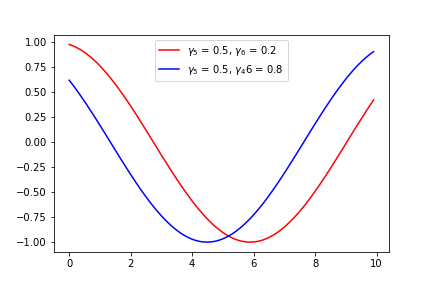
\includegraphics[width=\linewidth]{plots/scale_cos_g6.png}
			\caption{$f_{4}$ with different location parameter}
			\label{param_g6}
		\end{subfigure}
		\begin{subfigure}[b]{0.44\linewidth}
			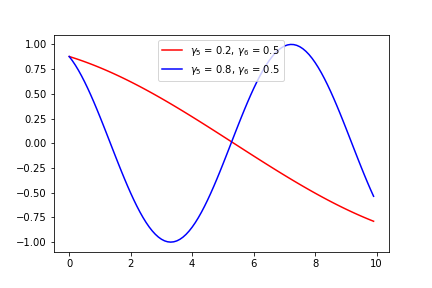
\includegraphics[width=\linewidth]{plots/scale_cos_g5.png}
			\caption{$f_{4}$ with different shape parameter}
			\label{param_g5}
		\end{subfigure}
		\label{trigo}
	\end{figure}
	
	In addition, we also consider two exponential functions:
	\begin{eqnarray*}
		\text{exp\_shift}: f_{5}\left( u_{t-1}, \gamma_{7}, \gamma_{8}\right) &=& 1-e^{-\gamma_{7}\left(u_{t-1}-\gamma_{8}\right)^{2}} \\
		\text{exp}: f_{6}\left( u_{t-1},\gamma _{9}, \gamma_{10}\right) &=& \gamma_{9} e^{-\gamma_{10}u_{t-1}^2},
	\end{eqnarray*} 
	where $\gamma_{7}, \gamma_{10}$ $\in(0, \infty)$. 
	The two exponential functions are bounded: $f_{5}\left(x_{t-1}^{\prime }\theta _{0},\gamma_{0}\right)$ lies in (0,1) and $f_{6}\left(x_{t-1}^{\prime }\theta _{0},\gamma _{0}\right)$ lies in (0, $\gamma_{9}$). 
	
	Figure \ref{exp1} and \ref{exp2} present the plots of $f_{5}\left(x_{t-1}^{\prime }\theta _{0},\gamma_{0}\right)$ and $f_{6}\left(x_{t-1}^{\prime }\theta _{0},\gamma_{0}\right)$. Even though both $f_5$ and $f_6$ are exponential functions, they have very different shapes. $f_5$ is an increasing function while $f_6$ is a decreasing function. We can see that $\gamma_{7}$ changes the steepness of $f_{5}\left(x_{t-1}^{\prime }\theta _{0},\gamma_{0}\right)$ (figure \ref{param_g7}) and $\gamma_{8}$ changes its position (figure \ref{param_g8}). And for $f_{6}\left(x_{t-1}^{\prime }\theta _{0},\gamma_{0}\right)$, $\gamma_{9}$ acts as the upper bound for the function and changes its position (figure \ref{param_g9}), while $\gamma_{10}$ changes its steepness (figure \ref{param_g10}).
	
	\begin{figure}[!htbp]
	\centering
	\caption{$f_{5}\left(x_{t-1}^{\prime }\theta _{0},\gamma_{0}\right)$ with different $\gamma$}
	\begin{subfigure}[b]{0.44\linewidth}
		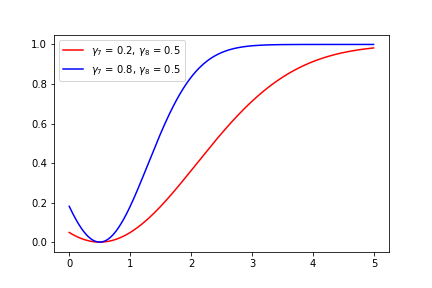
\includegraphics[width=\linewidth]{plots/scale_expshift_g7.png}
		\caption{$f_{5}$ with different $\gamma_{7}$}
		\label{param_g7}
	\end{subfigure}
	\begin{subfigure}[b]{0.44\linewidth}
		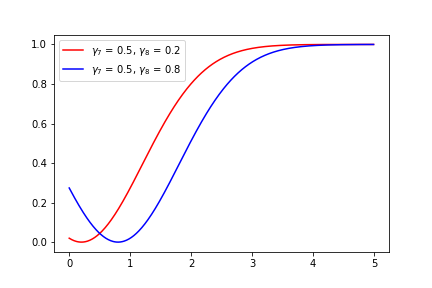
\includegraphics[width=\linewidth]{plots/scale_expshift_g8.png}
		\caption{$f_{5}$ with different $\gamma_{8}$}
		\label{param_g8}
	\end{subfigure}
	\label{exp1}
	\end{figure}

	\begin{figure}[!htbp]
	\centering
	\caption{$f_{6}\left(x_{t-1}^{\prime }\theta _{0},\gamma_{0}\right)$ with different $\gamma$}
	\begin{subfigure}[b]{0.44\linewidth}
		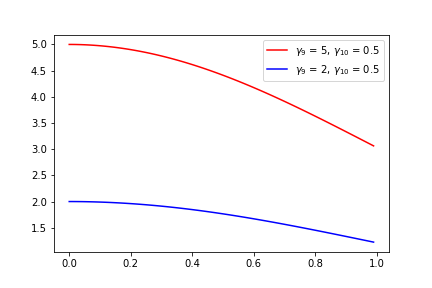
\includegraphics[width=\linewidth]{plots/scale_exp_g9.png}
		\caption{$f_{6}$ with different $\gamma_{7}$}
		\label{param_g9}
	\end{subfigure}
	\begin{subfigure}[b]{0.44\linewidth}
		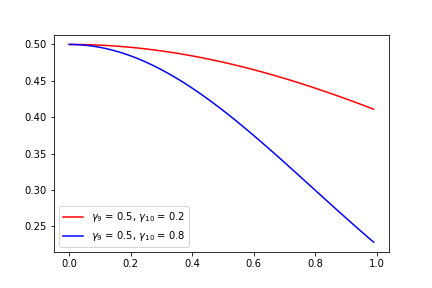
\includegraphics[width=\linewidth]{plots/scale_exp_g10.png}
		\caption{$f_{6}$ with different $\gamma_{8}$}
		\label{param_g10}
	\end{subfigure}
	\label{exp2}
	\end{figure}

In addition, we also consider a quadratic polynomial function:
$$
	\text{Polynomial}: f_{7}\left( u_{t-1},\gamma_{11}, \gamma_{12}, \gamma_{13}\right) = \gamma_{11}+ \gamma_{12}u_{t-1}+\gamma_{13}u_{t-1}^{2}
$$
It is a parabola where $\gamma_{11}$ decides the y-intercept and $\gamma_{13}$ changes the parabola's wideness.

The nonlinear functional forms we consider have included the bounded functions (the exponential functions), bounded periodic functions (trigonometric functions), and the unbounded function (polynomial function). 

\subsection{Initial Values (\textcolor{red}{re-write})}

As the gradient functions (\ref{gradient}) do not have a closed form solution, we will use an iterative procedure to estimate the model, which requires initial values. Most studies use 0 or true values as the initial values to start the procedure(\textcolor{red}{LR} here). Normally, true values provide the quickest and best convergence, but they are not known in empirical studies. And values that are close to the optimal values will tend to give a better convergence. 

Even though we do not known the optimal values beforehand, we can linearize our partially nonlinear model using Taylor expansion and estimate the linearized model to obtain better initial values. 

%to estimate the partially nonlinear model, we need to calculate the gradient functions (\ref{gradient}) first. But the gradient functions are nonlinear functions of both the variables and the parameters, so they do not have closed form solutions. Therefore, we use an iterative procedure to estimate the model. 
%To start the iterative procedure, 

Before applying Taylor expansion, we need to calculate the single-index $u_{t-1} = x^{\prime}_{t-1}\theta$. Since $x_1$ and $x_2$ are cointegrated, we can first estimate the following regression to get the cointegration vector $(1,-\hat{\eta})$:
$$
x_1 =\eta x_2 + e_t, \quad e_{t}\sim i.i.d.N\left( 0,1\right) ,\ \ t=2,...,T
$$
Then $\theta_0$ is given by normalizing the cointegration vector $(1,-\hat{\eta})$:
$$
\theta_{0} = (\dfrac{1}{\sqrt{1+\hat{\eta}^2}}, -\dfrac{\hat{\eta}}{\sqrt{1+\hat{\eta}^2}})
$$
which satisfies the constrain that $\|\theta_0\| = 1$. Then the single-index can be calculated as $\hat{u}_{t-1} = x^{\prime}_{t-1}\theta_0$.


As $\hat{u}_{t-1}$ has been estimated, we can apply Taylor expansion to approximate the nonlinear part $f\left( \hat{u}_{t-1},\gamma _{0}\right)$. For the two sine functions: $f_{1}\left( u_{t-1},\gamma _{0}\right) =\sin \left( u_{t-1}+\gamma_{1}\right)$ and $f_{3}\left( \gamma_{3}u_{t-1},\gamma _{4}\right) =\sin \left( \gamma_{3}u_{t-1}+\gamma_{4}\right)$, we can use their first order Taylor expansions and substitute $f_1$ and $f_3$ by: 
$$
\tilde{f_1} = \left( \hat{u}_{t-1}+\gamma_{1}\right) 
$$ 
$$
\tilde{f_3} = \left( \gamma_{3}\hat{u}_{t-1}+\gamma_{4}\right) 
$$ 

Then for the two cosine functions $f_{2}\left( u_{t-1},\gamma _{2}\right) =\cos \left(u_{t-1}+\gamma_{2}\right)$ and $f_{4}\left( \gamma _{5}u_{t-1}+\gamma_{6}\right) =\cos \left( \gamma_{5}u_{t-1}+\gamma_{6}\right)$, we approximate them using their second-order Taylor expansions:
$$
\tilde{f_2} = 1 - \left( \hat{u}_{t-1}+\gamma_{2}\right)^2
$$ 
$$
\tilde{f_4} =  1 - \left(\gamma _{5} \hat{u}_{t-1}+\gamma_{6}\right)^2
$$ 

Similarly, the two exponential functions $f_{5}\left( u_{t-1}, \gamma_{7}, \gamma_{8}\right) = 1-e^{-\gamma_{7}\left(u_{t-1}-\gamma_{8}\right)^{2}}$ and $f_{6}\left( u_{t-1},\gamma _{9}, \gamma_{10}\right) = \gamma_{9} e^{-\gamma_{10}u_{t-1}^2}$ can also be approximated by their first and second order Taylor expansions:

$$
\tilde{f_5} = \gamma_{7}(\hat{u}_{t-1} - \gamma_{8})^2
$$
$$
\tilde{f_6}= \gamma_{9}(1-\gamma_{10}\hat{u}_{t-1}^2 + \dfrac{\gamma_{10}^2 \hat{u}_{t-1}^4}{2})
$$
And for functional 7, the polynomial function, it is already a linear function when the single-index is known. Then we can substitute the nonlinear part $f_1$ to $f_6$ in model (\ref{PL model}) by $\tilde{f}_1$ to $\tilde{f}_6$ above. Therefore, the initial values of $( \beta, \gamma)$ for different functional forms can be calculated by estimating the following linear regressions:
\begin{align*}
	y_{t} & =  \gamma_{1}  + \hat{u}_{t-1} + \beta_{1}y_{t-1} + \beta_2w_{t-1} + e_t \\
	y_{t} & =  \gamma_{2}  + \hat{u}_{t-1} + \beta_{1}y_{t-1} + \beta_2w_{t-1} + e_t \\
	y_{t} & =  \gamma_{4}  + \gamma_{3}\hat{u}_{t-1} + \beta_{1}y_{t-1} + \beta_2w_{t-1} + e_t\\	
	y_{t} & =  \gamma_{6}  + \gamma_{5}\hat{u}_{t-1} + \beta_{1}y_{t-1} + \beta_2w_{t-1} + e_t \\
	y_{t} & =  \gamma_{7}\hat{u}_{t-1}^2 - 2\gamma_{7}\gamma_{8}\hat{u}_{t-1} + \gamma_{7}\gamma_{8}^2 + \beta_{1}y_{t-1} + \beta_2w_{t-1} + e_t \\
	y_{t} & =  \gamma_{9}(1-\gamma_{10}\hat{u}_{t-1}^2 + \dfrac{\gamma_{10}^2 \hat{u}_{t-1}^4}{2}) + \beta_{1}y_{t-1} + \beta_2w_{t-1} + e_t \\
	y_{t} & =  \gamma_{11}+ \gamma_{12}\hat{u}_{t-1}+\gamma_{13}\hat{u}_{t-1}^{2} +\beta_{1}y_{t-1} + \beta_2w_{t-1} + e_t
\end{align*}
where $\hat{u}_{t-1} = x^{\prime}_{t-1}\theta_0$ and $e_{t}\sim i.i.d.N\left( 0,1\right) ,\ \ t=2,...,T$.
% = \tilde{f_2}  + \beta_{1}y_{t-1} + \beta_2w_{t-1}

Together with $\theta_0$, we have calculated the initial values $\left(\theta_{0}, \beta_{0}, \gamma_{0} \right) $ for the iterative procedure. In the section below part, we can see that these initial values are better than random ones (for example, 0).

\subsection{Simulation Results}

\subsubsection{Compare Different Initial Values}

Table \ref{init values} shows the simulation results for the partially nonlinear model with polynomial $f\left( u_{t-1},\gamma\right)$:
$$
y_{t}  = \gamma_{11}+ \gamma_{12}{u}_{t-1}+\gamma_{13}{u}_{t-1}^{2} +\beta_{1}y_{t-1} + \beta_2w_{t-1} +e_t
$$
where ${u}_{t-1} = x^{\prime}_{t-1}\theta$ and $e_{t}\sim i.i.d.N\left( 0,1\right) ,\ \ t=2,...,T$.. From the table, we can see that the CLS estimators achieve the best convergence when using true values to start the iterative procedure. As shown in the bottom panel, the biases and standard deviations of the estimators are very low even when sample size T = 100. And it continues to decrease when sample size increases.

But when using 0 as initial values, the simulation performance is much worse. Take sample size T=500 and $\theta_1$ as an example, when using true values, the standard deviation of $\theta_1$ is 0.00029, while when initial values equal to 0, standard deviation of $\theta_1$ is 0.2855.  It also shows a worse convergence when sample size increase.

Even though the true values provide much better results, it is impossible for us to use true values to do the estimation in real world. Therefore, we adopt the Taylor initial values following the procedure in previous section to improve the finite sample performance. As we have approximated the model using Taylor expansions, the Taylor initial values we obtain are relatively close to the true values. Therefore we expect the results to be better than using random initial values. 

We can see from the first panel in table \ref{init values} that when using the Taylor initial values, the standard deviation of $\theta_1$ has decreased from 0.2855 (when initial values equals to 0) to 0.0004. It also shows a good convergence, where the biases and standard deviations both decreases when then sample size increases. Take the covariance of $\gamma$: cov($\gamma$) as an example, the covariance drops from 0.01029 when T = 100, to 0.00339 when T = 1000. 

Therefore, compare with previous studies, our Taylor initial values significantly improved the finite sample performance. We will then apply this method to our empirical studies later. 
% Table generated by Excel2LaTeX from sheet 'Sheet1'
\begin{table}[htbp]
	\centering
	\caption{Simulation Results for Polynomial $f\left( u_{t-1},\gamma\right)$ Using Different Initial Values}
	\begin{adjustbox}{max width=0.8\textwidth}
	\begin{tabular}{ccccccccc}
		\toprule
		&       & \multicolumn{1}{l}{$\theta_1$} & \multicolumn{1}{l}{$\theta_2$} & \multicolumn{1}{l}{$\beta_1$} & \multicolumn{1}{l}{$\beta_2$} & \multicolumn{1}{l}{$\gamma_1$} & \multicolumn{1}{l}{$\gamma_2$} & \multicolumn{1}{l}{$\gamma_3$} \\
		&       & \multicolumn{7}{c}{Initial Values = Taylor Initials} \\
		\midrule
		\multirow{3}[1]{*}{T=100} & Bias  & 0.00088 & 0.00026 & -0.00079 & 0.00029 & 0.00326 & -0.00064 & 0.00121 \\
		& std   & 0.00139 & 0.00105 & 0.00504 & 0.00504 & 0.00914 & 0.00451 & 0.00141 \\
		&       & \multicolumn{2}{c}{0.00244} & \multicolumn{2}{c}{0.00461} & \multicolumn{3}{c}{0.01029} \\
		\multirow{3}[0]{*}{T=500} & Bias  & -0.00013 & -0.00008 & -0.00040 & -0.00058 & 0.00063 & -0.00032 & 0.00146 \\
		& std   & 0.00041 & 0.00031 & 0.00068 & 0.00206 & 0.00436 & 0.00175 & 0.00043 \\
		&       & \multicolumn{2}{c}{0.00167} & \multicolumn{2}{c}{0.00167} & \multicolumn{3}{c}{0.00472} \\
		\multirow{3}[1]{*}{T=1000} & Bias  & -0.00005 & -0.00003 & -0.00025 & -0.00012 & 0.00035 & -0.00021 & 0.00087 \\
		& std   & 0.00026 & 0.00019 & 0.00043 & 0.00136 & 0.00319 & 0.00110 & 0.00026 \\
		&       & \multicolumn{2}{c}{0.00045} & \multicolumn{2}{c}{0.00110} & \multicolumn{3}{c}{0.00339} \\
		\midrule
		&       & \multicolumn{7}{c}{Initial Values = 0} \\
%		&       & \multicolumn{1}{l}{$\theta_1$} & \multicolumn{1}{l}{$\theta_2$} & \multicolumn{1}{l}{$\beta_1$} & \multicolumn{1}{l}{$\beta_2$} & \multicolumn{1}{l}{$\gamma_1$} & \multicolumn{1}{l}{$\gamma_2$} & \multicolumn{1}{l}{$\gamma_3$} \\
		\midrule
		\multirow{3}[1]{*}{T=100} & Bias  & 0.12214 & 0.35638 & 0.09401 & -0.27546 & 2.40099 & 0.19899 & -0.10567 \\
		& std   & 0.28186 & 0.45009 & 0.31824 & 1.10049 & 2.95226 & 0.67484 & 0.36090 \\
		&       & \multicolumn{2}{c}{0.51793} & \multicolumn{2}{c}{1.02441} & \multicolumn{3}{c}{0.17287} \\
		\multirow{3}[0]{*}{T=500} & Bias  & 0.13182 & 0.47163 & 0.19141 & -0.33712 & 2.25798 & 0.19733 & -0.18554 \\
		& std   & 0.28545 & 0.52487 & 0.38507 & 1.13323 & 2.50154 & 0.78597 & 0.38406 \\
		&       & \multicolumn{2}{c}{0.39734} & \multicolumn{2}{c}{0.57196} & \multicolumn{3}{c}{0.12342} \\
		\multirow{3}[1]{*}{T=1000} & Bias  & 0.15770 & 0.47870 & 0.21117 & -0.25275 & 2.34776 & 0.30953 & -0.20737 \\
		& std   & 0.26417 & 0.50324 & 0.04013 & 0.324009 & 0.21639 & 0.09167 & 0.06618 \\
		&       & \multicolumn{2}{c}{0.15924} & \multicolumn{2}{c}{0.10229} & \multicolumn{3}{c}{0.07233} \\
		\midrule
		&       & \multicolumn{7}{c}{Initial Values = True Values} \\
%		&       & \multicolumn{1}{l}{$\theta_1$} & \multicolumn{1}{l}{$\theta_2$} & \multicolumn{1}{l}{$\beta_1$} & \multicolumn{1}{l}{$\beta_2$} & \multicolumn{1}{l}{$\gamma_1$} & \multicolumn{1}{l}{$\gamma_2$} & \multicolumn{1}{l}{$\gamma_3$} \\
		\midrule
		\multirow{3}[1]{*}{T=100} & Bias  & 0.00008 & 0.00007 & -0.00170 & 0.00082 & 0.00368 & -0.00028 & 0.00080 \\
		& std   & 0.00127 & 0.00095 & 0.00196 & 0.00572 & 0.00735 & 0.00350 & 0.00174 \\
		&       & \multicolumn{2}{c}{0.00222} & \multicolumn{2}{c}{0.00261} & \multicolumn{3}{c}{0.00832} \\
		\multirow{3}[0]{*}{T=500} & Bias  & 0.00003 & 0.00002 & -0.00098 & 0.00085 & 0.00233 & -0.00003 & 0.00068 \\
		& std   & 0.00029 & 0.00022 & 0.00069 & 0.00192 & 0.00330 & 0.00135 & 0.00060 \\
		&       & \multicolumn{2}{c}{0.00050} & \multicolumn{2}{c}{0.00098} & \multicolumn{3}{c}{0.00362} \\
		\multirow{3}[1]{*}{T=1000} & Bias  & 0.00000 & 0.00001 & -0.00091 & 0.00084 & 0.00023 & -0.00003 & 0.00068 \\
		& std   & 0.00019 & 0.00014 & 0.00046 & 0.00133 & 0.00226 & 0.00090 & 0.00041 \\
		&       & \multicolumn{2}{c}{0.00033} & \multicolumn{2}{c}{0.00065} & \multicolumn{3}{c}{0.00247} \\
		\bottomrule
		\bottomrule
    \end{tabular}%
	\end{adjustbox}
	\label{init values}%
\end{table}%

\subsubsection{Results for Non-cointegrated $x_t$}

Table \ref{nonco-f12} presents the simulation results for non-cointegrated $x_t$ using $f_1 (u_{t-1}, \gamma_1)$ and $f_2 (u_{t-1}, \gamma_2)$. We can see from the table that both the NLSand CLS estimators converge when the sample size increases. And the CLS estimators perform better than the NLS estimators. For example, when T =1000, the bias and standard deviation of CLS estimator in $\beta_{1}$ in $f_1 (u_{t-1}, \gamma_1)$ is -0.00007 and 0.01574 respectively, but the values for the NLS estimator is 0.00835 and 0.01148. 

The covariance of $\theta$, $\beta$ and $\gamma$ are also smaller when the constraint is applied. Take the covariance of $\theta$ using  $f_2 (u_{t-1}, \gamma_2)$ as an example, cov($\hat{\theta}$) dropped from 0.70877 and 0.06903, to 0.00536 and 0.00283 when T = 500 and T = 1000.
% Table generated by Excel2LaTeX from sheet 'Sheet1'
\begin{table}[htbp]
	\centering
	\caption{Simulation Results for Non-cointegrated $x_t$ Using $f_1$ and $f_2$}
	\begin{adjustbox}{max width=\textwidth}
		\begin{tabular}{cccccccccccc}
		\toprule
		&       & \multicolumn{5}{c}{NLS}               & \multicolumn{5}{c}{Constrained-NLS} \\
		&       & $\theta_1$ & $\theta_2$ & $\beta_1$ & $\beta_2$ & $\gamma_1$ & $\theta_1$ & $\theta_2$ & $\beta_1$ & $\beta_2$ & $\gamma_1$ \\
		\midrule
		&       & \multicolumn{10}{c}{$f_1 (u_{t-1}, \gamma_1)$}                \\
		\midrule
		\multirow{3}[1]{*}{T = 100} & Bias  & 0.38379 & 0.18386 & 0.08270 & 0.48694 & -0.24803 & -0.00145 & -0.00116 & -0.00038 & 0.00089 & 0.04358 \\
		& std   & 0.50727 & 0.32935 & 0.13342 & 0.04772 & 0.46857 & 0.01523 & 0.01683 & 0.00122 & 0.01254 & 0.08301 \\
		&       & \multicolumn{2}{c}{0.63646} &       & \multicolumn{2}{c}{0.47723} & \multicolumn{2}{c}{0.02050} & \multicolumn{2}{c}{0.01191} &  \\
		\multirow{3}[0]{*}{T = 500} & Bias  & 0.38567 & 0.19677 & 0.07986 & 0.49866 & -0.23763 & -0.00408 & -0.00063 & -0.00012 & 0.00147 & 0.00911 \\
		& std   & 0.47487 & 0.30993 & 0.11830 & 0.01579 & 0.26452 & 0.00369 & 0.00432 & 0.00021 & 0.00364 & 0.03815 \\
		&       & \multicolumn{2}{c}{0.60420} &       & \multicolumn{2}{c}{0.26785} & \multicolumn{2}{c}{0.00574} & \multicolumn{2}{c}{0.00345} &  \\
		\multirow{3}[1]{*}{T = 1000} & Bias  & 0.03802 & 0.01811 & \textcolor[rgb]{ 0,  .439,  .753}{0.00835} & 0.04999 & -0.01991 & -0.00147 & -0.00026 & \textcolor[rgb]{ 0,  .439,  .753}{-0.00007} & 0.00100 & 0.00286 \\
		& std   & 0.04750 & 0.02966 & \textcolor[rgb]{ 0,  .439,  .753}{0.01148} & 0.00124 & 0.02029 & 0.01892 & 0.01693 & \textcolor[rgb]{ 0,  .439,  .753}{0.01574} & 0.02946 & 0.01798 \\
		&       & \multicolumn{2}{c}{0.05939} &       & \multicolumn{2}{c}{0.02050} & \multicolumn{2}{c}{0.00249} & \multicolumn{2}{c}{0.00279} &  \\
		\midrule
		\multicolumn{12}{c}{$f_1 (u_{t-1}, \gamma_2)$} \\
		\midrule
		\multirow{3}[1]{*}{T = 100} & Bias  & 0.44222 & 0.18241 & 0.08787 & 0.05589 & 0.47601 & -0.00424 & -0.00120 & -0.00100 & 0.00334 & 0.04116 \\
		& std   & 0.57804 & 0.33512 & 0.12559 & 0.02178 & 0.58834 & 0.01781 & 0.01584 & 0.00222 & 0.01433 & 0.08129 \\
		&       & \multicolumn{2}{c}{\textcolor[rgb]{ .329,  .51,  .208}{0.69034}} &       & \multicolumn{2}{c}{0.58181} & \multicolumn{2}{c}{\textcolor[rgb]{ .329,  .51,  .208}{0.02291}} & \multicolumn{2}{c}{0.01280} &  \\
		\multirow{3}[0]{*}{T = 500} & Bias  & 0.42377 & 0.16441 & 0.08132 & 0.05121 & 0.48900 & -0.00147 & -0.00052 & -0.00036 & 0.00208 & 0.00771 \\
		& std   & 0.59056 & 0.32840 & 0.13094 & 0.00719 & 0.55783 & 0.00396 & 0.00411 & 0.00065 & 0.00553 & 0.03370 \\
		&       & \multicolumn{2}{c}{\textcolor[rgb]{ .329,  .51,  .208}{0.70877}} &       & \multicolumn{2}{c}{0.55450} & \multicolumn{2}{c}{\textcolor[rgb]{ .329,  .51,  .208}{0.00536}} & \multicolumn{2}{c}{0.00493} &  \\
		\multirow{3}[1]{*}{T = 1000} & Bias  & 0.04422 & 0.01824 & 0.00559 & 0.04760 & 0.00879 & -0.00074 & -0.00032 & -0.00017 & 0.00096 & 0.00287 \\
		& std   & 0.05780 & 0.03351 & 0.00218 & 0.05883 & 0.01256 & 0.00222 & 0.00174 & 0.00040 & 0.00367 & 0.01557 \\
		&       & \multicolumn{2}{c}{\textcolor[rgb]{ .329,  .51,  .208}{0.06903}} & \multicolumn{2}{c}{0.05818} &       & \multicolumn{2}{c}{\textcolor[rgb]{ .329,  .51,  .208}{0.00283}} & \multicolumn{2}{c}{0.00328} &  \\
		\bottomrule
		\bottomrule
    	\end{tabular}%
		\end{adjustbox}
	\label{nonco-f12}%
\end{table}%

Table \ref{nonco-f12} presents the simulation results for non-cointegrated $x_t$ using $f_3 (u_{t-1}, \gamma_3, \gamma_4)$ and $f_4 (u_{t-1}, \gamma_5, \gamma_6)$. When compared with the NLS estimators, CLS estimators have smaller bias and deviations are smaller. The biases of $\theta_1$ in the case of CLS is -0.00177 while the value is 0.01467 in the case of NLS. And the CLS estimators also show a better convergence. As shown in the second panel, when sample size increases, the bias of $\beta_2$ decreases from 0.01092 to 0.00237. 

% Table generated by Excel2LaTeX from sheet 'Sheet1'
\begin{table}[htbp]
	\centering
	\caption{Simulation Results for Non-cointegrated $x_t$ Using $f_3$ and $f_4$}
	\begin{adjustbox}{max width=\textwidth}
	\begin{tabular}{cccccccccccccc}
		\toprule
		& \multicolumn{7}{c}{NLS}                               & \multicolumn{6}{c}{Constrained-NLS} \\
		&       & $\theta_1$ & $\theta_2$ & $\beta_1$ & $\beta_2$ & $\gamma_1$ & $\gamma_{2}$ & $\theta_1$ & $\theta_2$ & $\beta_1$ & $\beta_2$ & $\gamma_1$ & $\gamma_{2}$ \\
		\midrule
		&       & \multicolumn{12}{c}{$f_3 (u_{t-1}, \gamma_3, \gamma_4)$} \\
		\midrule
		\multirow{3}[1]{*}{T = 100} & Bias  & \textcolor[rgb]{ 0,  .439,  .753}{0.25080} & 0.11643 & 0.09701 & 0.09621 & -0.02764 & 0.04677 & \textcolor[rgb]{ 0,  .439,  .753}{-0.00512} & -0.00957 & 0.00367 & 0.04089 & 0.00023 & 0.00084 \\
		& std   & 0.42010 & 0.27514 & 0.10589 & 0.14919 & 0.02840 & 0.04952 & 0.12251 & 0.09119 & 0.02431 & 0.11107 & 0.01023 & 0.02126 \\
		&       & \multicolumn{2}{c}{0.49218} & \multicolumn{2}{c}{0.17846} & \multicolumn{2}{c}{0.02405} & \multicolumn{2}{c}{0.14820} & \multicolumn{2}{c}{0.11562} & \multicolumn{2}{c}{0.02353} \\
		\multirow{3}[0]{*}{T = 500} & Bias  & \textcolor[rgb]{ 0,  .439,  .753}{0.18672} & 0.09059 & 0.07042 & 0.11776 & -0.01412 & 0.02610 & \textcolor[rgb]{ 0,  .439,  .753}{-0.00682} & -0.00430 & 0.00062 & -0.00060 & -0.00083 & 0.00078 \\
		& std   & 0.37435 & 0.24955 & 0.09681 & 0.14953 & 0.01354 & 0.02486 & 0.02586 & 0.02294 & 0.00615 & 0.02334 & 0.00276 & 0.00475 \\
		&       & \multicolumn{2}{c}{0.44802} & \multicolumn{2}{c}{0.17453} & \multicolumn{2}{c}{0.01163} & \multicolumn{2}{c}{0.03783} & \multicolumn{2}{c}{0.02383} & \multicolumn{2}{c}{0.00561} \\
		\multirow{3}[1]{*}{T = 1000} & Bias  & \textcolor[rgb]{ 0,  .439,  .753}{0.01467} & 0.08110 & 0.05778 & 0.11680 & -0.00923 & 0.01717 & \textcolor[rgb]{ 0,  .439,  .753}{-0.00177} & -0.00162 & 0.00013 & -0.00149 & -0.00033 & 0.00038 \\
		& std   & 0.03410 & 0.23593 & 0.09100 & 0.14950 & 0.00941 & 0.01754 & 0.01433 & 0.01388 & 0.00406 & 0.01529 & 0.00166 & 0.00248 \\
		&       & \multicolumn{2}{c}{0.41141} & \multicolumn{2}{c}{0.17074} & \multicolumn{2}{c}{0.00825} & \multicolumn{2}{c}{0.02241} & \multicolumn{2}{c}{0.01568} & \multicolumn{2}{c}{0.00268} \\
		\midrule
		&       & \multicolumn{12}{c}{$f_4 (u_{t-1}, \gamma_5, \gamma_6)$} \\
		\midrule
		\multirow{3}[1]{*}{T = 100} & Bias  & 0.26070 & 0.13566 & 0.09572 & 0.10944 & -0.00129 & 0.00539 & -0.00839 & -0.00700 & 0.00085 & \textcolor[rgb]{ .329,  .51,  .208}{0.01092} & -0.02653 & 0.04272 \\
		& std   & 0.41629 & 0.28334 & 0.10132 & 0.14225 & 0.00287 & 0.01948 & 0.05009 & 0.04422 & 0.01350 & 0.05372 & 0.02733 & 0.04743 \\
		&       & \multicolumn{2}{c}{0.47705} & \multicolumn{2}{c}{0.17498} & \multicolumn{2}{c}{0.01708} & \multicolumn{2}{c}{0.06498} & \multicolumn{2}{c}{0.05641} & \multicolumn{2}{c}{0.02541} \\
		\multirow{3}[0]{*}{T = 500} & Bias  & 0.18304 & 0.09114 & 0.07063 & 0.12854 & -0.00039 & 0.00245 & -0.00153 & -0.00013 & -0.00044 & \textcolor[rgb]{ .329,  .51,  .208}{0.00449} & -0.01240 & 0.02233 \\
		& std   & 0.37174 & 0.24185 & 0.09417 & 0.14590 & 0.00071 & 0.00598 & 0.01367 & 0.01400 & 0.00352 & 0.01763 & 0.01216 & 0.02216 \\
		&       & \multicolumn{2}{c}{0.43332} & \multicolumn{2}{c}{0.17804} & \multicolumn{2}{c}{0.00530} & \multicolumn{2}{c}{0.02039} & \multicolumn{2}{c}{0.01847} & \multicolumn{2}{c}{0.01036} \\
		\multirow{3}[1]{*}{T = 1000} & Bias  & 0.01397 & 0.06411 & 0.05101 & 0.12171 & -0.00023 & 0.00163 & -0.00015 & 0.00049 & -0.00025 & \textcolor[rgb]{ .329,  .51,  .208}{0.00237} & -0.00777 & 0.01432 \\
		& std   & 0.03386 & 0.21123 & 0.08496 & 0.14666 & 0.00042 & 0.00383 & 0.00646 & 0.00684 & 0.00163 & 0.01559 & 0.00806 & 0.01490 \\
		&       & \multicolumn{2}{c}{0.40072} & \multicolumn{2}{c}{0.17760} & \multicolumn{2}{c}{0.00342} & \multicolumn{2}{c}{0.01009} & \multicolumn{2}{c}{0.01588} & \multicolumn{2}{c}{0.00699} \\
		\bottomrule
		\bottomrule
		\end{tabular}%
	\end{adjustbox}
	\label{nonco-f34}%
\end{table}%

Models with the two exponential functions (see table \ref{nonco-f56}) also show similar performance as other models. The NLS and CLS estimators converge when sample size increases and the CLS estimators perform better.

In table \ref{nonco-f7}, we can also see a good convergence and an improvement in finite sample performance when constraint and truncation have been applied. 

To conclude, for the non-cointegrated $x_t$, the proposed CLS estimators show a good convergence and a better performance than the normal NLS estimators. In the next section, we will investigate the performance of the estimators when $x_t$ is cointegrated.

% Table generated by Excel2LaTeX from sheet 'Sheet1'
\begin{table}[htbp]
	\centering
	\caption{Simulation Results for Non-cointegrated $x_t$ Using $f_5$ and $f_6$}
	\begin{adjustbox}{max width=\textwidth}
	\begin{tabular}{cccccccccccccc}
		\toprule
		& \multicolumn{7}{c}{NLS}                               & \multicolumn{6}{c}{Constrained-NLS} \\
		&       & $\theta_1$ & $\theta_2$ & $\beta_1$ & $\beta_2$ & $\gamma_1$ & $\gamma_{2}$ & $\theta_1$ & $\theta_2$ & $\beta_1$ & $\beta_2$ & $\gamma_1$ & $\gamma_{2}$ \\
		\midrule
		&       & \multicolumn{12}{c}{$f_5 (u_{t-1}, \gamma_7, \gamma_8)$} \\
		T = 100 & Bias  & \textcolor[rgb]{ .184,  .459,  .71}{0.12540} & 0.08285 & 0.03502 & 0.10013 & -0.00125 & 0.00465 & \textcolor[rgb]{ .184,  .459,  .71}{-0.01512} & -0.00850 & 0.00298 & 0.03600 & 0.00035 & 0.00010 \\
		& std   & 0.32644 & 0.22965 & 0.07947 & 0.14053 & 0.00291 & 0.01768 & 0.08939 & 0.09761 & 0.01671 & 0.10739 & 0.01028 & 0.02041 \\
		&       & \multicolumn{2}{c}{0.41166} & \multicolumn{2}{c}{0.16238} & \multicolumn{2}{c}{0.01553} & \multicolumn{2}{c}{0.13624} & \multicolumn{2}{c}{0.10882} & \multicolumn{2}{c}{0.02240} \\
		\multirow{3}[0]{*}{T = 500} & Bias  & \textcolor[rgb]{ .184,  .459,  .71}{0.07635} & 0.03312 & 0.02314 & 0.07846 & -0.00040 & 0.00256 & \textcolor[rgb]{ .184,  .459,  .71}{-0.00626} & -0.00533 & 0.00098 & 0.00020 & -0.00079 & 0.00069 \\
		& std   & 0.26124 & 0.15768 & 0.06617 & 0.13341 & 0.00061 & 0.00513 & 0.02448 & 0.02367 & 0.00617 & 0.02938 & 0.00270 & 0.00418 \\
		&       & \multicolumn{2}{c}{0.33234} & \multicolumn{2}{c}{0.15343} & \multicolumn{2}{c}{0.00456} & \multicolumn{2}{c}{0.03878} & \multicolumn{2}{c}{0.02994} & \multicolumn{2}{c}{0.00500} \\
		\multirow{3}[1]{*}{T = 1000} & Bias  & \textcolor[rgb]{ .184,  .459,  .71}{0.04853} & 0.02568 & 0.01525 & 0.06429 & -0.00021 & 0.00148 & \textcolor[rgb]{ .184,  .459,  .71}{-0.00145} & -0.00138 & 0.00006 & -0.00154 & -0.00033 & 0.00027 \\
		& std   & 0.21269 & 0.13821 & 0.05665 & 0.12720 & 0.00038 & 0.00335 & 0.01348 & 0.01318 & 0.00342 & 0.01526 & 0.00176 & 0.00231 \\
		&       & \multicolumn{2}{c}{0.27633} & \multicolumn{2}{c}{0.13912} & \multicolumn{2}{c}{0.00298} & \multicolumn{2}{c}{0.02050} & \multicolumn{2}{c}{0.01566} & \multicolumn{2}{c}{0.00267} \\
		\midrule
		&       & \multicolumn{12}{c}{$f_6 (u_{t-1}, \gamma_9, \gamma_{10})$} \\
		\midrule
		T = 100 & Bias  & 0.16972 & 0.09560 & 0.03762 & 0.09567 & -0.00140 & 0.00279 & -0.00253 & -0.00113 & 0.05286 & 0.11522 & -0.00797 & 0.02183 \\
		& std   & 0.36696 & 0.24840 & 0.08178 & 0.13985 & 0.00590 & 0.02946 & 0.02819 & 0.02091 & 0.17887 & 0.31808 & 0.00821 & 0.05086 \\
		&       & \multicolumn{2}{c}{\textcolor[rgb]{ .329,  .51,  .208}{0.45088}} & \multicolumn{2}{c}{0.15968} & \multicolumn{2}{c}{0.02947} & \multicolumn{2}{c}{\textcolor[rgb]{ .329,  .51,  .208}{0.04905}} & \multicolumn{2}{c}{0.36180} & \multicolumn{2}{c}{0.04597} \\
		\multirow{3}[0]{*}{T = 500} & Bias  & 0.13362 & 0.08659 & 0.03314 & 0.08628 & -0.00043 & 0.00218 & -0.00254 & -0.00179 & 0.01126 & 0.01520 & -0.00432 & 0.02071 \\
		& std   & 0.33483 & 0.23097 & 0.07623 & 0.13596 & 0.00139 & 0.01472 & 0.01036 & 0.00771 & 0.02667 & 0.13611 & 0.00234 & 0.02118 \\
		&       & \multicolumn{2}{c}{\textcolor[rgb]{ .329,  .51,  .208}{0.42320}} & \multicolumn{2}{c}{0.15627} & \multicolumn{2}{c}{0.01379} & \multicolumn{2}{c}{\textcolor[rgb]{ .329,  .51,  .208}{0.01806}} & \multicolumn{2}{c}{0.13714} & \multicolumn{2}{c}{0.01923} \\
		\multirow{3}[1]{*}{T = 1000} & Bias  & 0.08091 & 0.04687 & 0.02416 & 0.08304 & -0.00009 & 0.00082 & -0.00177 & -0.00128 & 0.00945 & -0.00417 & -0.00394 & 0.02014 \\
		& std   & 0.26874 & 0.18120 & 0.06819 & 0.13751 & 0.00020 & 0.00334 & 0.00698 & 0.00520 & 0.01713 & 0.08853 & 0.00161 & 0.01523 \\
		&       & \multicolumn{2}{c}{\textcolor[rgb]{ .329,  .51,  .208}{0.34376}} & \multicolumn{2}{c}{0.15229} & \multicolumn{2}{c}{0.00317} & \multicolumn{2}{c}{\textcolor[rgb]{ .329,  .51,  .208}{0.01218}} & \multicolumn{2}{c}{0.08865} & \multicolumn{2}{c}{0.01382} \\
		\bottomrule
		\bottomrule
    	\end{tabular}%
		\end{adjustbox}
\label{nonco-f56}%
\end{table}%


% Table generated by Excel2LaTeX from sheet 'Sheet1'
\begin{table}[htbp]
	\centering
	\caption{Simulation Results for Non-cointegrated $x_t$ Using $f_7$}
	\begin{adjustbox}{max width=\textwidth}
	\begin{tabular}{cccccccccccccccc}
		\toprule
		& \multicolumn{8}{c}{NLS}                                       & \multicolumn{7}{c}{Constrained-NLS} \\
		&       & theta & theta & beta  & beta  & gamma & gamma & gamma & theta & theta & beta  & beta  & gamma & gamma & gamma \\
		\midrule
		\multirow{3}[1]{*}{T = 100} & Bias  & \textcolor[rgb]{ 0,  .439,  .753}{0.02111} & -0.01598 & 30.87179 & -0.95731 & -0.01892 & -0.60074 & 0.72155 & \textcolor[rgb]{ 0,  .439,  .753}{0.00286} & 0.00084 & 0.06327 & -0.00989 & 0.00370 & -0.01088 & 0.00725 \\
		& std   & 0.36946 & 0.31152 & 0.74012 & 0.74312 & 0.29472 & 0.17836 & 0.14145 & 0.03604 & 0.02714 & 0.36089 & 0.05816 & 0.02418 & 0.03986 & 0.11360 \\
		&       & \multicolumn{2}{c}{0.48890} & \multicolumn{2}{c}{0.74443} & \multicolumn{3}{c}{0.14232} & \multicolumn{2}{c}{0.05138} & \multicolumn{2}{c}{0.36636} & \multicolumn{3}{c}{0.11006} \\
		\multirow{3}[0]{*}{T = 500} & Bias  & \textcolor[rgb]{ 0,  .439,  .753}{0.02983} & 0.02140 & 3.07132 & -0.65861 & 0.01327 & -0.05536 & 0.16146 & \textcolor[rgb]{ 0,  .439,  .753}{0.00066} & 0.00026 & 0.02231 & -0.00085 & 0.00025 & -0.00126 & 0.00019 \\
		& std   & 0.47050 & 0.43007 & 0.19241 & 0.285891 & 0.41959 & 0.47356 & 0.33892 & 0.00355 & 0.00347 & 0.11853 & 0.02182 & 0.00301 & 0.00422 & 0.02105 \\
		&       & 0.07039 &       & \multicolumn{2}{c}{0.19932} & \multicolumn{3}{c}{0.03417} & \multicolumn{2}{c}{0.00581} & \multicolumn{2}{c}{0.12056} & \multicolumn{3}{c}{0.02087} \\
		\multirow{3}[1]{*}{T = 1000} & Bias  & \textcolor[rgb]{ 0,  .439,  .753}{0.00261} & -0.00316 & 2.48519 & -0.17601 & 0.00291 & -0.01104 & -0.01521 & \textcolor[rgb]{ 0,  .439,  .753}{0.00014} & 0.00019 & 0.00743 & -0.00007 & 0.00014 & -0.00050 & -0.00008 \\
		& std   & 0.20383 & 0.17837 & 0.1113794 & 0.19016 & 0.20954 & 0.16493 & 0.19888 & 0.00155 & 0.00138 & 0.10818 & 0.01050 & 0.00141 & 0.00219 & 0.00929 \\
		&       & \multicolumn{2}{c}{\textcolor[rgb]{ .329,  .51,  .208}{0.00300}} & \multicolumn{2}{c}{\textcolor[rgb]{ .329,  .51,  .208}{0.11301}} & \multicolumn{3}{c}{\textcolor[rgb]{ .329,  .51,  .208}{0.01985}} & \multicolumn{2}{c}{\textcolor[rgb]{ .329,  .51,  .208}{0.00263}} & \multicolumn{2}{c}{\textcolor[rgb]{ .329,  .51,  .208}{0.10870}} & \multicolumn{3}{c}{\textcolor[rgb]{ .329,  .51,  .208}{0.00876}} \\
		\bottomrule
		\bottomrule
    	\end{tabular}%
	\end{adjustbox}
\label{nonco-f7}%
\end{table}%


\subsubsection{Simulation Results for Cointegrated $x_t$}
Table \ref{tab:s_f12} to \ref{s_f7} show the simulation results on co-integrated $x_t$ using Taylor initial values.  Table \ref{tab:s_f12} presents the results for model containing nonlinear component $f_1(u_{t-1}, \gamma_1) = \sin(u_t+\gamma_{1})$ and $f_2(u_{t-1}, \gamma_2) = = \cos(u_t+\gamma_{2})$. From the table we can see that the constrained CLS estimator performs better than the NLS estimator. Bias, standard deviation and covariance of the estimators are lower in the constrained least square case than in the nonlinear least square case. For example, for model containing $f_1$ , the absolute value of bias of $\theta_1$ is 0.00818 when using NLS and 0.00129 when using CLS estimator (sample size T = 1000). 

The estimators also show a good convergence. Take the covariance of $\gamma$ in the second panel as an example, the covariance of $\gamma$ decrease from 0.01916 to 0.00242 when sample size T rises from 100 to 1000. 
% Table generated by Excel2LaTeX from sheet 'Sheet1'
\begin{table}[htbp]
  \centering
  \caption{Simulation Results for Cointegrated $x_t$ Using Models with $f_1$ and $f_2$}
    \begin{adjustbox}{max width=\textwidth}
    \begin{tabular}{cccccccccccc}
    \toprule
          &       & \multicolumn{5}{c}{NLS}               & \multicolumn{5}{c}{Constrained-NLS} \\
          &       & $\theta_1$ & $\theta_2$ & $\beta_1$ & $\beta_2$ & $\gamma_1$ & $\theta_1$ & $\theta_2$ & $\beta_1$ & $\beta_2$ & $\gamma_1$ \\
    \midrule
    &       & \multicolumn{10}{c}{$f_1 (u_{t-1}, \gamma_1)$}                \\
    \midrule
    \multirow{3}[1]{*}{T = 100} & Bias  & 0.00221 & 0.01180 & -0.01443 & 0.01320 & 0.00447 & 0.01287 & 0.01004 & -0.01604 & -0.00325 & -0.02298 \\
          & std   & 0.09413 & 0.08928 & 0.05052 & 0.06048 & 0.52541 & 0.01474 & 0.01180 & 0.04778 & 0.05835 & 0.46140 \\
          &       & \multicolumn{2}{c}{0.08751} & \multicolumn{2}{c}{0.03648} &       & \multicolumn{2}{c}{0.02653} & \multicolumn{2}{c}{0.04417} &  \\
    \multirow{3}[0]{*}{T = 500} & Bias  & -0.00776 & 0.01514 & -0.01165 & 0.01131 & -0.00464 & 0.00247 & 0.00186 & -0.01223 & 0.00879 & -0.01146 \\
          & std   & 0.05713 & 0.04579 & 0.02192 & 0.02447 & 0.30383 & 0.00289 & 0.00219 & 0.02094 & 0.02295 & 0.29016 \\
          &       & \multicolumn{2}{c}{0.04800} & \multicolumn{2}{c}{0.01013} &       & \multicolumn{2}{c}{0.00508} & \multicolumn{2}{c}{0.00918} &  \\
    \multirow{3}[1]{*}{T = 1000} & Bias  & \textcolor[rgb]{ 0,  .439,  .753}{-0.00818} & 0.01622 & -0.01119 & 0.01126 & -0.00584 & \textcolor[rgb]{ 0,  .439,  .753}{0.00129} & 0.00097 & -0.01176 & 0.01021 & -0.02066 \\
          & std   & 0.06111 & 0.04695 & 0.01541 & 0.01690 & 0.29261 & 0.00149 & 0.00112 & 0.01526 & 0.01632 & 0.27447 \\
          &       & \multicolumn{2}{c}{0.05325} & \multicolumn{2}{c}{0.00590} &       & \multicolumn{2}{c}{0.00262} & \multicolumn{2}{c}{0.00471} &  \\
    \midrule
    &       & \multicolumn{10}{c}{$f_2 (u_{t-1}, \gamma_2)$}                \\
    \midrule
    \multirow{3}[1]{*}{T = 100} & Bias  & 0.00069 & 0.00276 & -0.00646 & 0.00180 & 0.03309 & -0.00189 & -0.00192 & 0.00104 & -0.00143 & 0.04245 \\
          & std   & 0.04767 & 0.03619 & 0.03458 & 0.04583 & 0.12469 & 0.02647 & 0.02972 & 0.01103 & 0.01648 & 0.08817 \\
          &       & \multicolumn{2}{c}{0.08369} & \multicolumn{2}{c}{0.04306} &       & \multicolumn{2}{c}{0.03984} & \multicolumn{2}{c}{\textcolor[rgb]{ .329,  .51,  .208}{0.01916}} &  \\
    \multirow{3}[0]{*}{T = 500} & Bias  & 0.00068 & 0.00075 & -0.01248 & 0.01028 & -0.00206 & -0.00010 & -0.00026 & -0.00049 & 0.00061 & 0.00770 \\
          & std   & 0.01564 & 0.01175 & 0.01493 & 0.02015 & 0.05825 & 0.00622 & 0.00698 & 0.00272 & 0.00421 & 0.04282 \\
          &       & \multicolumn{2}{c}{0.02738} & \multicolumn{2}{c}{0.01652} &       & \multicolumn{2}{c}{0.00927} & \multicolumn{2}{c}{\textcolor[rgb]{ .329,  .51,  .208}{0.00518}} &  \\
    \multirow{3}[1]{*}{T = 1000} & Bias  & -0.00012 & 0.00005 & -0.01275 & 0.01034 & 0.00029 & -0.00015 & 0.00087 & -0.00041 & 0.00051 & 0.00100 \\
          & std   & 0.01206 & 0.00905 & 0.01188 & 0.01482 & 0.04136 & 0.00329 & 0.00330 & 0.00156 & 0.00191 & 0.02102 \\
          &       & \multicolumn{2}{c}{0.02110} & \multicolumn{2}{c}{0.01129} &       & \multicolumn{2}{c}{0.00476} & \multicolumn{2}{c}{\textcolor[rgb]{ .329,  .51,  .208}{0.00242}} &  \\
    \bottomrule
    \bottomrule
    \end{tabular}%
    \end{adjustbox}
  \label{tab:s_f12}%
\end{table}%


Similarly for $f_3(u_{t-1},\gamma_3, \gamma_4) = \sin(\gamma_3 u_t+\gamma_{4})$ and $f_4(\gamma_5 u_{t-1}, \gamma_6) = \cos(\gamma_5 u_t+\gamma_{6})$, both NLS and CLS estimators converge and the CLS estimators perform better. For example, in the first panel of table \ref{s_f34}, the absolute value of bias of $\theta_1$ using $f_3(u_{t-1}, \gamma_3, \gamma_4)$ decreases from 0.00219 to 0.00062 in the case of CLS and drops from 0.01336 to 0.00201 in the case of NLS. 

And in most cases, the CLS estimators have smaller bias, standard deviation and covariance. As shown in the second panel of table \ref{s_f34}, the covariance of CLS estimator $\gamma$ (cov($\hat{\gamma}$) ) when sample size T = 100 is slightly higher than the bias of the NLS estimator (0.19193 for CLS and 0.17287 for NLS), but when T increases to 500 and 1000, cov($\hat{\gamma}$) of the CLS estimator become smaller (0.05015 for CLS when T = 1000, and 0.09848 for NLS).


%Take $\theta$ in table \ref{tab:s_f12} as an example, for $f_1(u_{t-1}, \gamma_0)$, when sample size T=1000, the bias of $\theta_1$ and $\theta_2$ using CLS is 0.00129 and 0.00097 respectively, while the corresponding values using normal NLS is -0.00818 and 0.01622. Similarly for $f_2(u_{t-1}, \gamma_0)$, when T = 1000, the standard deviation for $\theta$ is 0.00476 in the case of CLS and 0.02110 in the case of NLS.  



% Table generated by Excel2LaTeX from sheet 'Sheet1'
\begin{table}[htbp]
  \centering
  \caption{Simulation Results for Cointegrated $x_t$ Using Models with $f_3$ and $f_4$}
    \begin{adjustbox}{max width=\textwidth}
    \begin{tabular}{cccccccccccccc}
    \toprule
          &       & \multicolumn{6}{c}{NLS}                       & \multicolumn{6}{c}{Constrained-NLS} \\
          &       & $\theta_1$ & $\theta_2$ & $\beta_1$ & $\beta_2$ & $\gamma_1$ & $\gamma_2$ & $\theta_1$ & $\theta_2$ & $\beta_1$ & $\beta_2$ & $\gamma_1$ & $\gamma_2$ \\
    \midrule
    &       & \multicolumn{10}{c}{$f_3 (u_{t-1}, \gamma_3, \gamma_4)$}                \\
    \midrule
    \multirow{3}[1]{*}{T = 100} & Bias  & \textcolor[rgb]{ 0,  .439,  .753}{-0.01336} & -0.00146 & 0.00040 & 0.00012 & 0.00258 & 0.03875 & \textcolor[rgb]{ 0,  .439,  .753}{-0.00219} & 0.00367 & -0.01027 & 0.00355 & 0.00143 & -0.00586 \\
          & std   & 0.09908 & 0.10823 & 0.01118 & 0.01976 & 0.02365 & 0.11074 & 0.07270 & 0.05655 & 0.03583 & 0.05240 & 0.06347 & 0.12251 \\
          &       & \multicolumn{2}{c}{0.14788} & \multicolumn{2}{c}{0.02250} & \multicolumn{2}{c}{0.11450} & \multicolumn{2}{c}{0.12888} & \multicolumn{2}{c}{0.05136} & \multicolumn{2}{c}{0.13895} \\
    \multirow{3}[0]{*}{T = 500} & Bias  & \textcolor[rgb]{ 0,  .439,  .753}{-0.00561} & -0.00664 & -0.00106 & 0.00100 & 0.00074 & 0.00084 & \textcolor[rgb]{ 0,  .439,  .753}{0.00039} & 0.00178 & -0.01354 & 0.00635 & -0.00269 & -0.00414 \\
          & std   & 0.02504 & 0.02534 & 0.00283 & 0.00462 & 0.00631 & 0.03351 & 0.03891 & 0.02937 & 0.01772 & 0.02257 & 0.02483 & 0.04649 \\
          &       & \multicolumn{2}{c}{0.03833} & \multicolumn{2}{c}{0.00539} & \multicolumn{2}{c}{0.03384} & \multicolumn{2}{c}{0.06821} & \multicolumn{2}{c}{0.02083} & \multicolumn{2}{c}{0.05447} \\
    \multirow{3}[1]{*}{T = 1000} & Bias  & \textcolor[rgb]{ 0,  .439,  .753}{-0.00201} & -0.00204 & -0.00048 & 0.00044 & 0.00039 & -0.00138 & \textcolor[rgb]{ 0,  .439,  .753}{0.00062} & 0.00143 & -0.01299 & 0.00738 & -0.00171 & -0.00021 \\
          & std   & 0.01434 & 0.01451 & 0.00197 & 0.00230 & 0.00392 & 0.01576 & 0.03144 & 0.02371 & 0.01291 & 0.01631 & 0.01754 & 0.03414 \\
          &       & \multicolumn{2}{c}{0.02283} & \multicolumn{2}{c}{0.00277} & \multicolumn{2}{c}{0.01611} & \multicolumn{2}{c}{0.05511} & \multicolumn{2}{c}{0.01493} & \multicolumn{2}{c}{0.04048} \\
    \midrule
    &       & \multicolumn{10}{c}{$f_4 (u_{t-1}, \gamma_5, \gamma_6$)}                \\
    \midrule
    \multirow{3}[1]{*}{T = 100} & Bias  & -0.00462 & 0.00898 & -0.00485 & 0.00572 & 0.00210 & 0.03106 & -0.00283 & 0.00192 & 0.00022 & -0.00015 & -0.01107 & -0.00375 \\
          & std   & 0.10139 & 0.10403 & 0.03259 & 0.05225 & 0.01558 & 0.10063 & 0.06346 & 0.04934 & 0.01071 & 0.02085 & 0.05994 & 0.18408 \\
          &       & \multicolumn{2}{c}{0.14118} & \multicolumn{2}{c}{0.04906} & \multicolumn{2}{c}{\textcolor[rgb]{ .329,  .51,  .208}{0.17287}} & \multicolumn{2}{c}{0.11249} & \multicolumn{2}{c}{0.02418} & \multicolumn{2}{c}{\textcolor[rgb]{ .329,  .51,  .208}{0.19193}} \\
    \multirow{3}[0]{*}{T = 500} & Bias  & -0.00586 & 0.00356 & -0.01139 & 0.01223 & 0.00094 & 0.00065 & -0.01064 & -0.00614 & -0.00082 & 0.00065 & -0.00232 & -0.02078 \\
          & std   & 0.01965 & 0.02729 & 0.01540 & 0.02242 & 0.00549 & 0.03119 & 0.04250 & 0.03141 & 0.00315 & 0.00483 & 0.02115 & 0.07684 \\
          &       & \multicolumn{2}{c}{0.03187} & \multicolumn{2}{c}{0.02015} & \multicolumn{2}{c}{\textcolor[rgb]{ .329,  .51,  .208}{0.12557}} & \multicolumn{2}{c}{0.07384} & \multicolumn{2}{c}{0.00576} & \multicolumn{2}{c}{\textcolor[rgb]{ .329,  .51,  .208}{0.07694}} \\
    \multirow{3}[1]{*}{T = 1000} & Bias  & -0.00286 & 0.00068 & -0.00984 & 0.01005 & 0.00026 & -0.00096 & -0.00967 & -0.00599 & -0.00052 & 0.00048 & -0.00040 & -0.01090 \\
          & std   & 0.01282 & 0.01323 & 0.01171 & 0.01616 & 0.00364 & 0.01763 & 0.03508 & 0.02570 & 0.00194 & 0.00233 & 0.01420 & 0.05158 \\
          &       & \multicolumn{2}{c}{0.01564} & \multicolumn{2}{c}{0.01282} & \multicolumn{2}{c}{\textcolor[rgb]{ .329,  .51,  .208}{0.09848}} & \multicolumn{2}{c}{0.06074} & \multicolumn{2}{c}{0.00272} & \multicolumn{2}{c}{\textcolor[rgb]{ .329,  .51,  .208}{0.05015}} \\
    \bottomrule
    \bottomrule
    \end{tabular}%
    \end{adjustbox}
  \label{s_f34}%
\end{table}%

For the models containing two exponential functions $f_{5}\left( u_{t-1}, \gamma_{7}, \gamma_{8}\right) = 1-e^{-\gamma_{7}\left(u_{t-1}-\gamma_{8}\right)^{2}}$ and $f_{6}\left( u_{t-1},\gamma _{9}, \gamma_{10}\right) = \gamma_{9} e^{-\gamma_{10}u_{t-1}^2}$, we can see that the NLS estimators does not have good convergence, but after applying constraint, the CLS perform much better. For example, in the case of NLS, the biases of $\beta_{1}$ is -0.00060 and is -0.00051 when T = 100 and 1000 respectively. But in the case of CLS, the absolute values of bias of $\beta_{1}$ drop from 0.08371 to 0.00105. 

The CLS estimators also shows a significant decrease in the covariance. Take $\beta$ in $f_{6}\left( u_{t-1},\gamma _{9}, \gamma_{10}\right)$ as an example, the covariance of the CLS estimator is 0.00263 and that of the NLS estimator is 0.01184.
 
% Table generated by Excel2LaTeX from sheet 'Sheet1'
\begin{table}[htbp]
  \centering
  \caption{Simulation Results for Cointegrated $x_t$ Using Models with $f_5$ and $f_6$}
    \begin{adjustbox}{max width=\textwidth}
    \begin{tabular}{cccccccccccccc}
    \toprule
          &       & \multicolumn{6}{c}{NLS}                       & \multicolumn{6}{c}{Constrained-NLS} \\
          &       & $\theta_1$ & $\theta_2$ & $\beta_1$ & $\beta_2$ & $\gamma_1$ & $\gamma_2$ & $\theta_1$ & $\theta_2$ & $\beta_1$ & $\beta_2$ & $\gamma_1$ & $\gamma_2$ \\
    \midrule
    &       & \multicolumn{10}{c}{$f_5 (u_{t-1},\gamma_7, \gamma_8)$}                \\
    \midrule
    \multirow{3}[1]{*}{T = 100} & Bias  & 0.14852 & 0.07716 & \textcolor[rgb]{ 0,  .439,  .753}{-0.00060} & -0.00069 & 0.03979 & 0.09704 & 0.00049 & 0.00707 & \textcolor[rgb]{ 0,  .439,  .753}{-0.08371} & 0.00270 & 0.05869 & 0.11357 \\
    & std   & 0.36721 & 0.25730 & 0.00983 & 0.01876 & 0.08946 & 0.14248 & 0.08064 & 0.06468 & 0.03280 & 0.04974 & 0.22359 & 0.36681 \\
    &       & \multicolumn{2}{c}{0.47514} & \multicolumn{2}{c}{0.02122} & \multicolumn{2}{c}{0.16524} & \multicolumn{2}{c}{0.14459} & \multicolumn{2}{c}{0.04685} & \multicolumn{2}{c}{0.44678} \\
    \multirow{3}[0]{*}{T = 500} & Bias  & 0.06033 & 0.02538 & \textcolor[rgb]{ 0,  .439,  .753}{-0.00080} & 0.00085 & 0.03530 & 0.09690 & -0.00189 & 0.00011 & \textcolor[rgb]{ 0,  .439,  .753}{-0.01111} & 0.00823 & 0.00059 & 0.02411 \\
    & std   & 0.25251 & 0.16061 & 0.00290 & 0.00427 & 0.08116 & 0.14316 & 0.03955 & 0.02972 & 0.01524 & 0.01987 & 0.04029 & 0.17323 \\
    &       & \multicolumn{2}{c}{0.30811} & \multicolumn{2}{c}{0.00490} & \multicolumn{2}{c}{0.16249} & \multicolumn{2}{c}{0.06920} & \multicolumn{2}{c}{0.01641} & \multicolumn{2}{c}{0.17454} \\
    \multirow{3}[1]{*}{T = 1000} & Bias  & 0.04737 & 0.02568 & \textcolor[rgb]{ 0,  .439,  .753}{-0.00051} & 0.00050 & 0.02912 & 0.08033 & -0.00377 & -0.00197 & \textcolor[rgb]{ 0,  .439,  .753}{-0.00105} & 0.00843 & 0.00041 & -0.00583 \\
          & std   & 0.21925 & 0.14210 & 0.00204 & 0.00215 & 0.07485 & 0.13657 & 0.02952 & 0.02203 & 0.01198 & 0.01481 & 0.02361 & 0.11419 \\
          &       & \multicolumn{2}{c}{0.28125} & \multicolumn{2}{c}{0.00249} & \multicolumn{2}{c}{0.15389} & \multicolumn{2}{c}{0.05151} & \multicolumn{2}{c}{0.01177} & \multicolumn{2}{c}{0.11498} \\
    \midrule
    &       & \multicolumn{10}{c}{$f_6 (u_{t-1}, \gamma_9, \gamma_{10})$}                \\
    \midrule
    \multirow{3}[1]{*}{T = 100} & Bias  & 0.29939 & 0.12435 & -0.00836 & 0.00577 & 0.09685 & 0.86918 & 0.00239 & 0.00565 & -0.00015 & 0.00038 & 0.10008 & 0.10486 \\
          & std   & 0.44703 & 0.31855 & 0.03431 & 0.04555 & 0.26677 & 1.16532 & 0.06176 & 0.04835 & 0.01144 & 0.01696 & 0.10519 & 0.14436 \\
          &       & \multicolumn{2}{c}{0.52722} & \multicolumn{2}{c}{\textcolor[rgb]{ .329,  .51,  .208}{0.04150}} & \multicolumn{2}{c}{1.23387} & \multicolumn{2}{c}{0.10976} & \multicolumn{2}{c}{\textcolor[rgb]{ .329,  .51,  .208}{0.01892}} & \multicolumn{2}{c}{0.16633} \\
    \multirow{3}[0]{*}{T = 500} & Bias  & 0.20686 & 0.12096 & -0.01268 & 0.01065 & 0.01278 & 0.33971 & -0.00633 & -0.00314 & -0.00108 & 0.00100 & 0.08506 & 0.11410 \\
          & std   & 0.39309 & 0.27335 & 0.01578 & 0.02035 & 0.09200 & 0.81052 & 0.04018 & 0.03030 & 0.00304 & 0.00424 & 0.09984 & 0.14511 \\
          &       & \multicolumn{2}{c}{0.47572} & \multicolumn{2}{c}{\textcolor[rgb]{ .329,  .51,  .208}{0.01677}} & \multicolumn{2}{c}{0.82640} & \multicolumn{2}{c}{0.07041} & \multicolumn{2}{c}{\textcolor[rgb]{ .329,  .51,  .208}{0.00456}} & \multicolumn{2}{c}{0.16128} \\
    \multirow{3}[1]{*}{T = 1000} & Bias  & 0.18891 & 0.09882 & -0.01164 & 0.01017 & 0.00430 & 0.17839 & -0.00107 & -0.00681 & -0.00047 & 0.00036 & 0.07620 & 0.11676 \\
          & std   & 0.37535 & 0.25110 & 0.01210 & 0.01538 & 0.06249 & 0.54192 & 0.03382 & 0.02468 & 0.00180 & 0.00239 & 0.09744 & 0.14438 \\
          &       & \multicolumn{2}{c}{0.45836} & \multicolumn{2}{c}{\textcolor[rgb]{ .329,  .51,  .208}{0.01184}} & \multicolumn{2}{c}{0.56098} & \multicolumn{2}{c}{0.05847} & \multicolumn{2}{c}{\textcolor[rgb]{ .329,  .51,  .208}{0.00263}} & \multicolumn{2}{c}{0.16354} \\
    \bottomrule
    \bottomrule
    \end{tabular}%
    \end{adjustbox}
  \label{s_f56}%
\end{table}%


Table \ref{s_f7} presents the simulation results for the model containing polynomial function $f_{7}\left( u_{t-1},\gamma_{11}, \gamma_{12}, \gamma_{13}\right) = \gamma_{11}+ \gamma_{12}u_{t-1}+\gamma_{13}u_{t-1}^{2}$. Both NLS and CLS estimators have good convergence and the CLS shows a better performance for $\beta$ and $\gamma$. 

As for the convergence, take $\beta_{1}$ as an example, the absolute value of bias for the NLS estimator $\hat{\beta}$ decreases from 0.00056 to 0.00001 as sample size T increases from 100 to 1000. At the same time, the absolute value of bias for the CLS estimator $\bar{\beta}$ decreases from 0.00079 to 0.00025. 

The constraint and truncation conditions we applied improve the finite sample performance for all the estimators, but the effect is more significant for the estimator $\gamma$. For example, when T = 1000, the covariance of $\beta$ in the case of NLS is 0.00190 and the value is 0.00110 in the case of CLS. And for the covariance of $\gamma$, the value in the case of CLS is 0.00339, which is much lower than 0.01231 in the case of NLS.

% Table generated by Excel2LaTeX from sheet 'Sheet1'
\begin{table}[htbp]
  \centering
  \caption{Simulation Results for Cointegrated $x_t$ Using Models with $f_7$}
    \begin{adjustbox}{max width=\textwidth}
    \begin{tabular}{cccccccccccccccc}
    \toprule
          &       & \multicolumn{7}{c}{NLS}                               & \multicolumn{7}{c}{Constrained-NLS} \\
          &       & $\theta_1$ & $\theta_2$ & $\beta_1$ & $\beta_2$ & $\gamma_1$ & $\gamma_2$ & $\gamma_3$ & $\theta_1$ & $\theta_2$ & $\beta_1$ & $\beta_2$ & $\gamma_1$ & $\gamma_2$ & $\gamma_3$ \\
    \midrule
    \multirow{3}[1]{*}{T = 100} & Bias  & 0.00018 & -0.00018 & \textcolor[rgb]{ 0,  .439,  .753}{-0.00056} & 0.00037 & 0.02711 & -0.00147 & 0.00020 & 0.00088 & 0.00026 & \textcolor[rgb]{ 0,  .439,  .753}{-0.00079} & 0.00029 & 0.00326 & -0.00064 & 0.00121 \\
          & std   & 0.00407 & 0.00335 & 0.00171 & 0.01482 & 0.07001 & 0.00886 & 0.00308 & 0.00139 & 0.00105 & 0.00161 & 0.00504 & 0.00914 & 0.00451 & 0.00141 \\
          &       & \multicolumn{2}{c}{0.00528} & \multicolumn{2}{c}{0.01502} & \multicolumn{3}{c}{0.07063} & \multicolumn{2}{c}{0.00244} & \multicolumn{2}{c}{0.00461} & \multicolumn{3}{c}{0.01029} \\
    \multirow{3}[0]{*}{T = 500} & Bias  & 0.00006 & 0.00003 & \textcolor[rgb]{ 0,  .439,  .753}{-0.00003} & 0.00024 & 0.00261 & -0.00072 & 0.00026 & -0.00013 & -0.00008 & \textcolor[rgb]{ 0,  .439,  .753}{-0.00040} & -0.00058 & 0.00063 & -0.00032 & 0.00146 \\
          & std   & 0.00051 & 0.00040 & 0.00039 & 0.00354 & 0.01664 & 0.00315 & 0.00047 & 0.00041 & 0.00031 & 0.00068 & 0.00206 & 0.00436 & 0.00175 & 0.00043 \\
          &       & \multicolumn{2}{c}{0.00068} & \multicolumn{2}{c}{0.00357} & \multicolumn{3}{c}{0.01695} & \multicolumn{2}{c}{0.00071} & \multicolumn{2}{c}{0.00167} & \multicolumn{3}{c}{0.00472} \\
    \multirow{3}[1]{*}{T = 1000} & Bias  & 0.00008 & 0.00004 & \textcolor[rgb]{ 0,  .439,  .753}{-0.00001} & -0.00014 & 0.00218 & -0.00008 & -0.00006 & -0.00005 & -0.00003 & \textcolor[rgb]{ 0,  .439,  .753}{-0.00025} & -0.00012 & 0.00035 & -0.00021 & 0.00087 \\
          & std   & 0.00026 & 0.00015 & 0.00015 & 0.00194 & 0.01219 & 0.00173 & 0.00020 & 0.00026 & 0.00019 & 0.00043 & 0.00136 & 0.00319 & 0.00110 & 0.00026 \\
          &       & \multicolumn{2}{c}{0.00032} & \multicolumn{2}{c}{\textcolor[rgb]{ .329,  .51,  .208}{0.00190}} & \multicolumn{3}{c}{\textcolor[rgb]{ .329,  .51,  .208}{0.01231}} & \multicolumn{2}{c}{0.00045} & \multicolumn{2}{c}{\textcolor[rgb]{ .329,  .51,  .208}{0.00110}} & \multicolumn{3}{c}{\textcolor[rgb]{ .329,  .51,  .208}{0.00339}} \\
    \bottomrule
    \bottomrule
    \end{tabular}%
    \end{adjustbox}
  \label{s_f7}%
\end{table}%

From the simulation results above, we can conclude that:
\begin{enumerate}
    \item Both the NLS and CLS estimators converge when sample size increases. But the constrained least square method tend to give better convergence in certain cases.
    
    \item The CLS consistently perform better than the normal NLS for most functional forms. This implies that the constraint and truncation condition we proposed in section 2 do help improve the finite sample performances. 
\end{enumerate}

If we compare models with the 7 different functional forms,  we find that the polynomial functional form tend to provide the best results but models with the two exponential functions do not perform as well as other ones. 

As shown in table \ref{s_f7}, the standard deviation of $\theta$ using CLS is 0.00045 when T=1000, which is much lower than this value in other functional cases(for example, the corresponding value is 0.00262 in $f_1(u_{t-1}, \gamma_0)$ and 0.00476 in $f_2(u_{t-1}, \gamma_0)$). 

When compare the simulation results for non-cointegrated $x_t$ with the results for cointegrated $x_t$ (see table below), we can also see that the models using cointegrated $x_t$ have a better finite sample performance. Therefore, in next section, we will focus on models with cointegrated predictors. In addition, as the CLS estimators consistently provide better performance, we will focus on the constrained least square method in the empirical study.

% Table generated by Excel2LaTeX from sheet 'Sheet1'
\begin{table}[htbp]
	\centering
	\caption{Simulation Results for Cointegrated $x_t$ and Non-cointegrated $x_t$ Using $f_7$}
	\begin{adjustbox}{max width=\textwidth}
	\begin{tabular}{cccccccccccccccc}
		\toprule
		&       & \multicolumn{7}{c}{Cointegrated $x_t$}                               & \multicolumn{7}{c}{Non-cointegrated $x_t$} \\
		&       & $\theta_1$ & $\theta_2$ & $\beta_1$ & $\beta_2$ & $\gamma_1$ & $\gamma_2$ & $\gamma_3$ & $\theta_1$ & $\theta_2$ & $\beta_1$ & $\beta_2$ & $\gamma_1$ & $\gamma_2$ & $\gamma_3$ \\
		\midrule
		\multirow{3}[1]{*}{T = 100} & Bias  & \multicolumn{1}{r}{\textcolor[rgb]{ 0,  .439,  .753}{0.00088}} & \multicolumn{1}{r}{0.00026} & \multicolumn{1}{r}{-0.00079} & \multicolumn{1}{r}{0.00029} & \multicolumn{1}{r}{0.00326} & \multicolumn{1}{r}{-0.00064} & \multicolumn{1}{r}{0.00121} & \textcolor[rgb]{ 0,  .439,  .753}{0.00286} & 0.00084 & 0.06327 & -0.00989 & 0.00370 & -0.01088 & 0.00725 \\
		& std   & \multicolumn{1}{r}{0.00139} & \multicolumn{1}{r}{0.00105} & \multicolumn{1}{r}{0.00161} & \multicolumn{1}{r}{0.00504} & \multicolumn{1}{r}{0.00914} & \multicolumn{1}{r}{0.00451} & \multicolumn{1}{r}{0.00141} & 0.03604 & 0.02714 & 0.36089 & 0.05816 & 0.02418 & 0.03986 & 0.11360 \\
		&       & \multicolumn{2}{c}{0.00244} & \multicolumn{2}{c}{0.00461} & \multicolumn{3}{c}{0.01029} & \multicolumn{2}{c}{0.05138} & \multicolumn{2}{c}{0.36636} & \multicolumn{3}{c}{0.11006} \\
		\multirow{3}[0]{*}{T = 500} & Bias  & \multicolumn{1}{r}{\textcolor[rgb]{ 0,  .439,  .753}{-0.00013}} & \multicolumn{1}{r}{-0.00008} & \multicolumn{1}{r}{-0.0004} & \multicolumn{1}{r}{-0.00058} & \multicolumn{1}{r}{0.00063} & \multicolumn{1}{r}{-0.00032} & \multicolumn{1}{r}{0.00146} & \textcolor[rgb]{ 0,  .439,  .753}{0.00066} & 0.00026 & 0.02231 & -0.00085 & 0.00025 & -0.00126 & 0.00019 \\
		& std   & \multicolumn{1}{r}{0.00041} & \multicolumn{1}{r}{0.00031} & \multicolumn{1}{r}{0.00068} & \multicolumn{1}{r}{0.00206} & \multicolumn{1}{r}{0.00436} & \multicolumn{1}{r}{0.00175} & \multicolumn{1}{r}{0.00043} & 0.00355 & 0.00347 & 0.11853 & 0.02182 & 0.00301 & 0.00422 & 0.02105 \\
		&       & \multicolumn{2}{c}{0.00071} & \multicolumn{2}{c}{0.00167} & \multicolumn{3}{c}{0.00472} & \multicolumn{2}{c}{0.00581} & \multicolumn{2}{c}{0.12056} & \multicolumn{3}{c}{0.02087} \\
		\multirow{3}[1]{*}{T = 1000} & Bias  & \multicolumn{1}{r}{\textcolor[rgb]{ 0,  .439,  .753}{-0.00005}} & \multicolumn{1}{r}{-0.00003} & \multicolumn{1}{r}{-0.00025} & \multicolumn{1}{r}{-0.00012} & \multicolumn{1}{r}{0.00035} & \multicolumn{1}{r}{-0.00021} & \multicolumn{1}{r}{0.00087} & \textcolor[rgb]{ 0,  .439,  .753}{0.00014} & 0.00019 & 0.00743 & -0.00007 & 0.00014 & -0.00050 & -0.00008 \\
		& std   & \multicolumn{1}{r}{0.00026} & \multicolumn{1}{r}{0.00043} & \multicolumn{1}{r}{0.00043} & \multicolumn{1}{r}{0.00136} & \multicolumn{1}{r}{0.00319} & \multicolumn{1}{r}{0.0011} & \multicolumn{1}{r}{0.00026} & 0.00155 & 0.00138 & 0.10818 & 0.01050 & 0.00141 & 0.00219 & 0.00929 \\
		&       & \multicolumn{2}{c}{0.00045} & \multicolumn{2}{c}{0.0011} & \multicolumn{3}{c}{0.00339} & \multicolumn{2}{c}{0.00263} & \multicolumn{2}{c}{0.10870} & \multicolumn{3}{c}{0.00876} \\
		\bottomrule
		\bottomrule
    \end{tabular}%
	\end{adjustbox}
	\label{s_f7}%
\end{table}%



\section{Empirical Study}
We have examined the finite sample properties in the previous section using Monte Carlo simulation study. To illustrate the use of our partially nonlinear model in the real world, we conduct the in-sample and out-of-sample prediction exercises using U.S. stock market returns data.
The datasets is available from Amit Goyal's website and it is quarterly data ranging from 1956 Q1 to 2018 Q4 . 

The dependent variable, stock returns, are measured as continuously compound returns on the S\&P 500 index. 
Predictors used in \cite{welch2008comprehensive} include dividend-price ratio (log), dividend yield (log), earnings-price ratio (log), dividend-payout ratio (log), and other 11 predictors. 

In our study, we want to evaluate the performance of the partially nonlinear models when the non-stationary predictors are co-integrated, therefore we choose the following 4 variable pairs from the \cite{welch2008comprehensive} datasets (as in \cite{zhou2018semiparametric}) and another set of variable from \cite{lettau2001consumption}, which have all been found to be co-integrated : 
\begin{itemize}
	\item co1: dividend-price ratio (dp) and dividend yield (dy). 
	
	Dividend-price ratio is the difference between the log of dividends and the log of stock prices; dividend yield is the difference between the log of dividends and the log of lagged stock prices.
	
	\item co2: T-bill rate (tbl) and long-term yield (lty).
	
	T-bill rate is the interest rate on a three-month Treasury bill; long-term yield stands for the long-term government bond yield.
	
	\item co3: dividend-price ratio and earning-price ratio.
	
	The earning-price ratio is the difference between the log of earnings on the S\&P 500 index and the log of stock prices.
	
	\item co4: baa- and aaa-rated corporate bonds yields. 
			
\end{itemize}

Figure \ref{variables} plots the time series of the co-integrated variable pairs. It is clear that the variables in each plot are not stationary and have similar shape. Especially for the first pair, "co1", the d/p ratio and the dividend yield are very close to each other. 

\begin{figure}[!htbp]
	\centering
	\caption{Time Series Plots of Co-integrated Variables}
	\begin{subfigure}[b]{0.4\linewidth}
		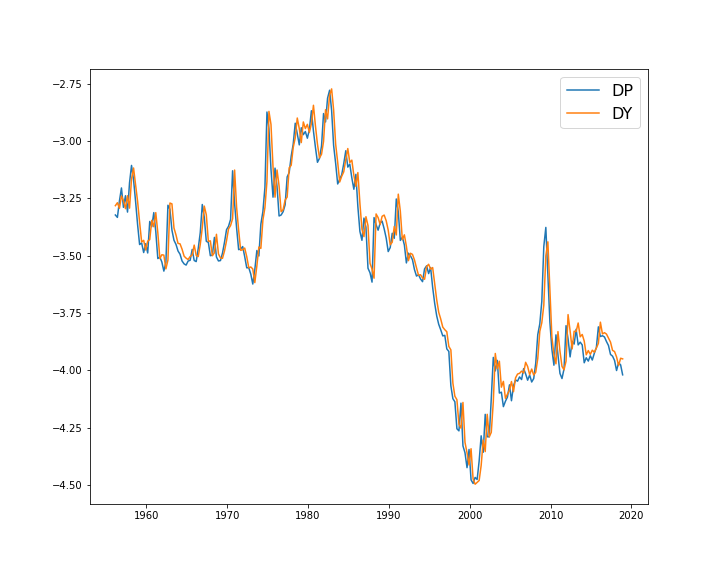
\includegraphics[width=1.2\linewidth]{plots/co1.png}
		\caption{co1}
	\end{subfigure}
	\begin{subfigure}[b]{0.4\linewidth}
		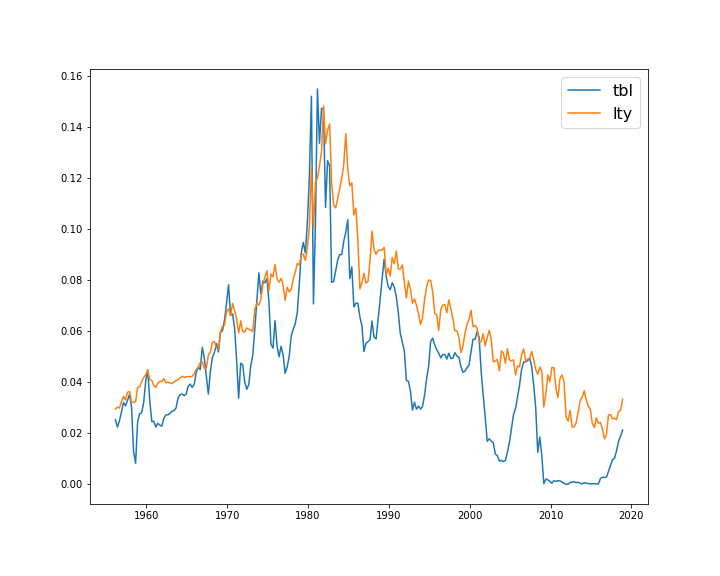
\includegraphics[width=1.2\linewidth]{plots/co2.png}
		\caption{co2}
	\end{subfigure}
	\begin{subfigure}[b]{0.4\linewidth}
		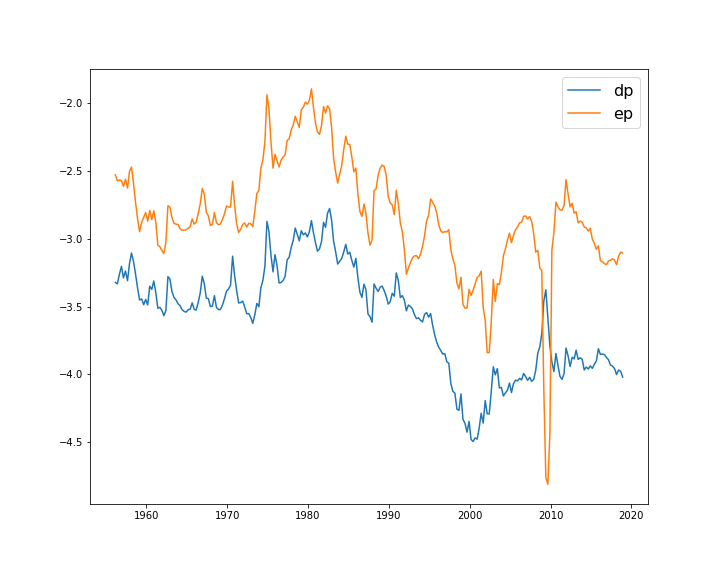
\includegraphics[width=1.2\linewidth]{plots/co3.png}
		\caption{co3}
	\end{subfigure}
	\begin{subfigure}[b]{0.4\linewidth}
		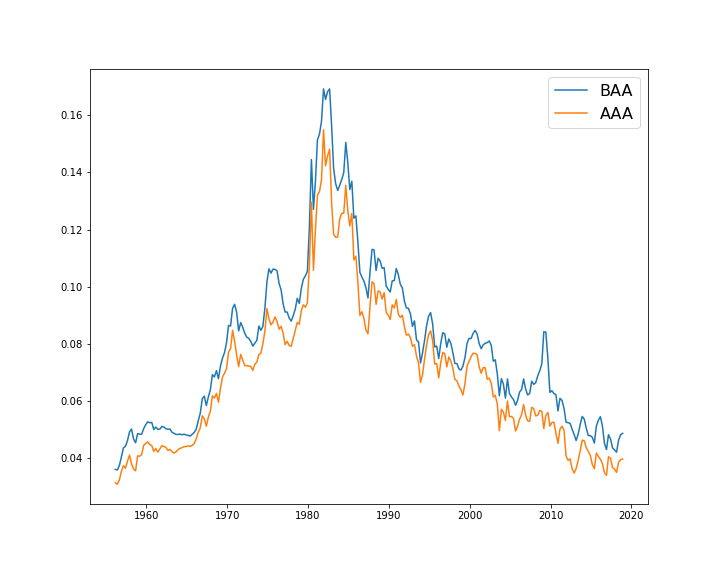
\includegraphics[width=1.2\linewidth]{plots/co4.png}
		\caption{co4}
	\end{subfigure}
	\label{variables}
\end{figure}

Figure \ref{cay} shows the three variables used in \cite{lettau2001consumption}. It is clear that log consumption, log asset wealth and log labor income share a common stochastic trend.

\begin{figure}[!htbp]
	\centering
	\caption{"cay" variable}
	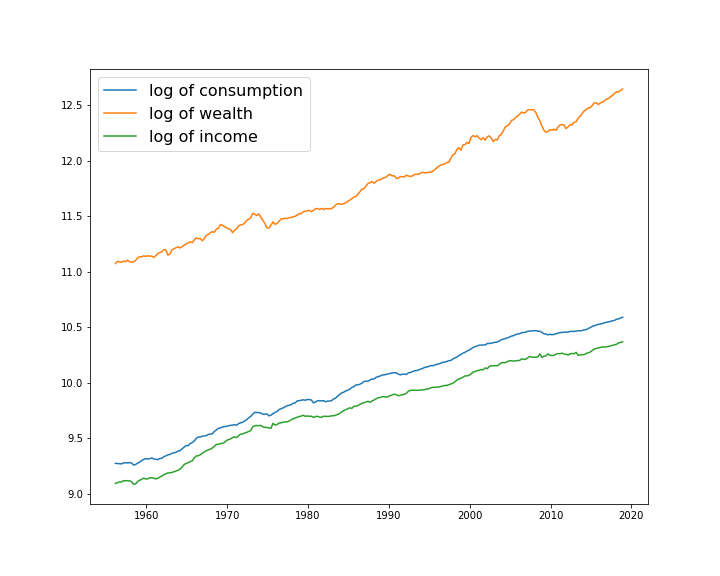
\includegraphics[width=0.5\linewidth]{plots/cay.png}
	\label{cay}
\end{figure}

Apart from the non-stationary variables, the partially nonlinear models also include stationary predictors: the lagged stock return ($y_{t-1}$) and the regression residual (the "cay" variable, hereafter) from the study of \cite{lettau2001consumption}. In their study, they show that the three variables are cointegrated and share a common trend. The deviations from this shared trend is stationary and can be used as a predictor for stock return. Figure \ref{station_vs} below presents the two stationary variables (\textcolor{red}{???}). 

\begin{figure}[!htbp]
	\centering
	\caption{Time Series Plots of Stationary Variables}
	\begin{subfigure}[b]{0.48\linewidth}
		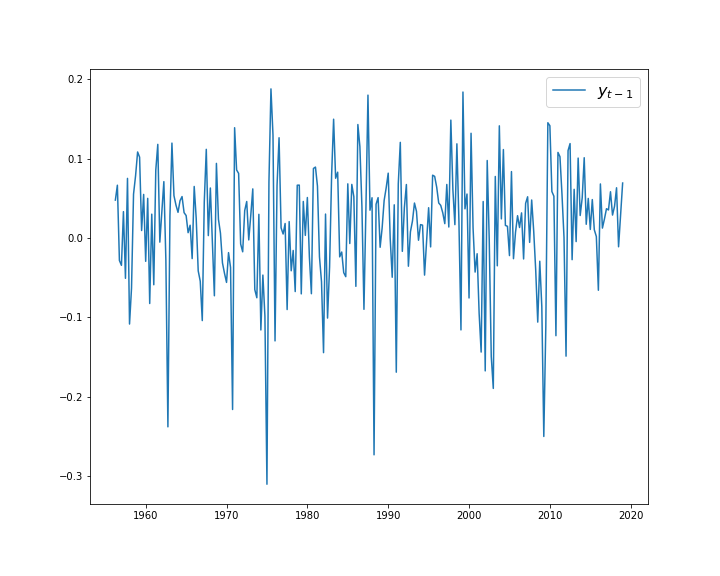
\includegraphics[width = \linewidth]{plots/ylag.png}
		\caption{lag of dependent variable}
	\end{subfigure}
	\begin{subfigure}[b]{0.48\linewidth}
		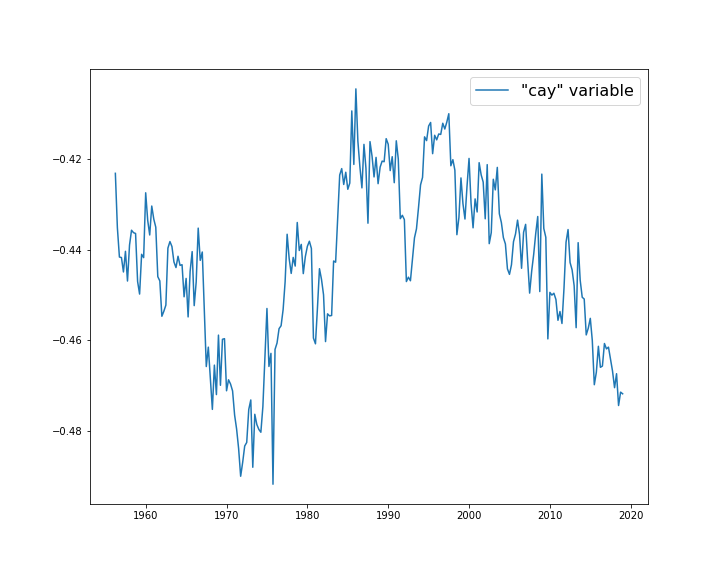
\includegraphics[width = \linewidth]{plots/new_cay.png}
		\caption{"cay" variable}
	\end{subfigure}
	\label{station_vs}
\end{figure}


Therefore in the partially nonlinear models we consider: 
$$
y_{t} = \beta_{1} y_{t-1} + \beta_{2} w_{t-1} + f\left( x_{t-1}^{\prime }\theta,\gamma\right) +e_{t}, \quad
e_{t}\sim i.i.d.N\left( 0,1\right) ,\ \ t=2,...,T,
$$
the dependent variable, $y_t$, is the equity premium defined as the S\&P500 value-weighted log excess returns. $y_{t-1}$ is the lagged equity premium, $x_{t-1}$ are the co-integrated variables from \cite{zhou2018semiparametric}, and $w_{t-1}$ is the regression residual, the "cay" variable, from the \cite{lettau2001consumption}. 

In terms of the nonlinear part $f\left( x_{t-1}^{\prime }\theta,\gamma\right)$, we consider the following 7 nonlinear functions that have been discussed in the simulation before, which includes trigonometric functions, exponential functions and polynomial functions. And these partially nonlinear models in the empirical study can be written as:
\begin{eqnarray*}
	\text{sin}: g_{1}\left( {u}_{t-1},\gamma _{1}\right) &=& \beta z_{t-1}^{\prime} + \sin \left( {u}_{t-1}+\gamma_{1}\right),  \\
	\text{cos}: g_{2}\left( {u}_{t-1},\gamma _{2}\right) &=& \beta z_{t-1}^{\prime} + \cos \left( {u}_{t-1}+\gamma_{2}\right), \\
	\text{scale\_sin}: g_{3}\left( {u}_{t-1},\gamma_{3}, \gamma_{4}\right) &=& \beta z_{t-1}^{\prime} + \sin \left( \gamma_{3}{u}_{t-1}+\gamma_{4}\right),  \\
	\text{scale\_cos}: g_{4}\left( {u}_{t-1},\gamma_{5}, \gamma_{6}\right) &=& \beta z_{t-1}^{\prime} + \cos \left( \gamma_{5}{u}_{t-1}+\gamma_{6}\right), \\
	\text{exp\_shift}: g_{5}\left( {u}_{t-1},,\gamma_{7}, \gamma_{8}\right) &=&  \beta z_{t-1}^{\prime} + 1-e^{-\gamma_{7}\left({u}_{t-1}-\gamma_{8}\right)^{2}} \\
	\text{exp}: g_{6}\left( {u}_{t-1},\gamma_{9}, \gamma_{10}\right) &=&  \beta z_{t-1}^{\prime} + \gamma_{9} e^{-\gamma_{10}{u}_{t-1}^2}  \\
	\text{Polynomial}: g_{7}\left( \hat{u}_{t-1},\gamma_{11}, \gamma_{12}, \gamma_{13}\right) &=& \beta z_{t-1}^{\prime} + \gamma_{11}+ \gamma_{12}{u}_{t-1}+\gamma_{13}{u}_{t-1}^{2}
\end{eqnarray*}%
where $\beta = (\beta_{1}, \beta_{2})$, $ z_{t-1}^{\prime } = (y_{t-1}, w_{t-1})$, and $u_{t-1} =  x_{t-1}^{\prime }\theta$.

% \noindent\textcolor{green}{\rule{16cm}{1mm}}

In addition, we also include a linear functional form with single-index:
$$
\text{constrained\_linear}: g_8\left( u_{t-1},\gamma_{14}, \gamma_{15}\right) = \gamma_{14} +\beta z_{t-1}^{\prime} + \gamma_{15}(x_{1,t-1}\theta _{1} + x_{2,t-1}\theta _{2}).
$$
It is a special case of the polynomial function $g_7$ where  $\gamma_{13} = 0$.

For all the 8 functional forms, we set $\theta^2_{1}+\theta_{2}^2 = 1$ and will adopt the constrained nonlinear least square method described in section 2 to estimate. But as mentioned before, when minimizing the nonlinear least squares:
$$
S_{T}(\beta, \theta, \gamma)=\sum_{t=1}^{T}\left(y_{t}-g\left(u_{t-1}, \gamma\right)\right)^{2}
$$

The gradient equation:
$$
\frac{\partial S_{T}(\alpha)}{\partial \alpha}
$$
does not have a closed solution, so we need to use an iterative algorithm. To implement the iterative algorithm, we must choose a vector of initial values to start. As discussed in the simulation study, we could use Taylor expansion to approximate the partially nonlinear models and choose initial values by estimating the approximated linear models. We first nee to estimate the following linear regression to get $\hat{\eta}$:
$$
x_1 = \eta x_2 + e_t, \quad e_{t}\sim i.i.d.N\left( 0,1\right) ,\ \ t=2,...,T
$$
where $x_1$ and $x_2$ are the non-stationary co-integrated variables. 
Then, the initial values for $\theta$ is $\theta_{0} = (\dfrac{1}{\sqrt{1+\eta^2}}, \dfrac{-\eta}{\sqrt{1+\eta^2}})$. 
As $\theta_{0}$ is known, we can calculate $\hat{u}_{t-1}$.

Then following what we have done in section 3, we bring $\hat{u_{t-1}}$ back into $f\left( u_{t-1},\gamma \right)$ and substitute the nonlinear function $f\left( u_{t-1},\gamma \right)$ by its first or second order Taylor expansion and estimate the following linear regression to obtain the initial values for $\beta$ and $\gamma$.
\begin{eqnarray*}
	\text{sin}: \tilde{g_{1}}\left( \hat{u}_{t-1},\gamma _{1}\right) &=& \left( \gamma_{1} +\hat{u}_{t-1}\right) + \beta z_{t-1}^{\prime},  \\
	\text{cos}: \tilde{g_{2}}\left( \hat{u}_{t-1},\gamma _{2}\right) &=& 1 - \left( \gamma_{2} + \hat{u}_{t-1}\right)^2  + \beta z_{t-1}^{\prime}, \\
	\text{sin\_scaled}: \tilde{g_{3}}\left( \hat{u}_{t-1},\gamma_{3},\gamma_{4}\right) &=& \gamma_{4}  + \gamma_{3}\hat{u}_{t-1} + \beta z_{t-1}^{\prime},  \\
	\text{cos\_scaled}: \tilde{g_{4}}\left( \hat{u}_{t-1},,\gamma_{5},\gamma_{6}\right) &=& 1 - \left( \gamma_{6} + \gamma_{5}\hat{u}_{t-1}\right)^2  + \beta z_{t-1}^{\prime}, \\
	\text{exp\_shift}: \tilde{g_{5}}\left( \hat{u}_{t-1},\gamma_{7},\gamma_{8}\right) &=&  \gamma_{7}\hat{u}_{t-1}^2 - 2\gamma_{8}\gamma_{7}\hat{u}_{t-1} + \gamma_{7}\gamma_{8}^2 + \beta z_{t-1}^{\prime} \\
	\text{exp}: \tilde{g_{6}}\left( \hat{u}_{t-1},\gamma_{9},\gamma_{10}\right) &=&  \gamma_{9}(1-\gamma_{10}\hat{u}_{t-1}^2 + \dfrac{\gamma_{10}^2 \hat{u}_{t-1}^4}{2}) + \beta z_{t-1}^{\prime}, \\
	\text{Polynomial}: \tilde{g_{7}}\left( \hat{u}_{t-1},,\gamma_{11},\gamma_{12},\gamma_{13}\right) &=& \gamma_{11}+ \gamma_{12}\hat{u}_{t-1}+\gamma_{13}\hat{u}_{t-1}^{2}+\beta z_{t-1}^{\prime}, \\
	\text{constrained\_linear}: \tilde{g_{8}}\left( \hat{u}_{t-1},\gamma_{14}, \gamma_{15}\right) &=& \gamma_{14}+ \gamma_{15}\hat{u}_{t-1}+\beta z_{t-1}^{\prime}
\end{eqnarray*}%
where $\beta = (\beta_{1}, \beta_{2})$, $ z_{t-1}^{\prime } = (y_{t-1}, w_{t-1})$.

In the simulation section, we have shown that by using Taylor-initials, the convergence of the estimators have improved significantly. In this section, we will investigate the empirical performances of our partially nonlinear models using these Taylor-initials.

% \noindent\textcolor{green}{\rule{16cm}{1mm}}

% Following \cite{welch2008comprehensive}, we use the sample mean model as a benchmark. The sample mean model can be defined as:

% $$
% y_t= \dfrac{1}{t-1}\sum_{1}^{t-1}y_i
% $$

% \noindent\textcolor{green}{\rule{16cm}{1mm}}


% In addition, we also adopt auto-regressive models as additional benchmarks for comparison. We consider 3 forms of AR models: AR(1) model, AR(2) model, and an AR(1) model with the cay variable.
% \begin{itemize}
% 	\item AR1:
% 	$$
% 	y_t = \beta_{1}y_{t-1} + \epsilon_t
% 	$$
% 	\item AR2:
% 	$$
% 	y_t =\beta_{1,0} y_{t-1} + \beta_{2,0} y_{t-2} + \epsilon_t
% 	$$
% 	\item AR1 model with "cay" variable (AR\_cay):
% 	$$
% 	y_t = \beta_{1,0}y_{t-1} + \beta_{2,0}cay_{t-1} + \epsilon_t
% 	$$
% \end{itemize}

% We also include a nonlinear model which has the same nonlinear part as in the partially nonlinear model, but does not include the lagged dependent variable and the "cay" variable.
% \begin{itemize}
% 	\item Nonlinear single-index model (NLS):
% 	$$
% 	y_{t} = f\left( x_{t-1}^{\prime }\theta _{0},\beta _{0}\right) + \epsilon_{t},
% 	$$
% \end{itemize}
% where $\epsilon_{t}\sim i.i.d.N\left( 0,1\right)$ for all the benchmark models.

\subsection{In-sample Results}
In this section, we use the complete sample from 1956 Q1 to 2018 Q4 to investigate the in-sample performances of our partially nonlinear models. The full sample results can be found in the appendix, table \ref{full}. In this section, we use in-sample $r^2$ to examine the in-sample performance of our models.
The in-sample $R^2_{IS}$ is defined as:
\begin{equation}
	R_{IS}^{2}=1-\frac{\sum_{t=1}^{n}\left(y_{t}-\widehat{y}_{t}\right)^{2}}{\sum_{t=1}^{n}\left(y_{t}-\bar{y}\right)^{2}}
\end{equation}
where $y_t$ is the observed stock return in time t, $\bar{y}$ is the predicted return from the benchmark model, and $\hat{y_{t}}$ is the corresponding predicted stock return. 

% The sample mean model can be defined as:
% $$
% \bar{y_t}= \dfrac{1}{t-1}\sum_{1}^{t-1}y_i.
% $$

$R^2_{IS}$ can also be rewritten as:
\begin{equation}
	R_{IS}^{2}=1-\frac{MSE_{CLS}}{MSE_{bm}}
	\label{Ris}
\end{equation}
where $MSE_{bm}$ is the mean squared error of benchmark model and $\mathrm{MSE}_{CLS}=1 / n \sum_{t=1}^{n}\left(y_{t}-\hat{y_t}\right)^{2}$ is the mean squared error of our partially nonlinear models.
In equation (\ref{Ris}), if $R^2_{IS}$ for a given model is positive, it indicates that the model outperforms the benchmark model, and the bigger the value is, the better the corresponding model performs.

In the study of \cite{welch2008comprehensive}, they found that sample mean is a competitive model in stock return prediction. Therefore, we use the sample mean model as the benchmark. To compare our models with some commonly used time series models and the nonlinear model we used in chapter 2:

\begin{itemize}
	\item Sample mean model: 
	$$
	y_t= \dfrac{1}{t-1}\sum_{1}^{t-1}y_i
	$$
	\item AR1:
	$$
	y_t = \beta_{1}y_{t-1} + \epsilon_t
	$$
	\item AR2:
	$$
	y_t =\beta_{1} y_{t-1} + \beta_{2} y_{t-2} + \epsilon_t
	$$
	\item AR1 model with "cay" variable:
	$$
	y_t = \beta_{1}y_{t-1} + \beta_{2}cay_{t-1} + \epsilon_t
	$$
	\item Nonlinear single-index model:
	$$
	y_{t} = f\left( x_{t-1}^{\prime }\theta,\beta\right) + \epsilon_{t},
	$$
	
	where $e_{t}\sim i.i.d.N\left( 0,1\right).$
\end{itemize}

The results of $R^2_{IS}$ against sample mean model is reported in table \ref{ins_R2}. Among the 8 functional forms, $g_3$, $g_4$, $g_5$, $g_7$ and $g_8$ provide positive $R^2_{IS}$ for all 4 variable combinations, which means the 5 functional forms have better in-sample performances than historical benchmark. And for $g_1$, $g_2$ and $g_6$, they can outperform sample mean model for some of the variable combinations. 


% and we find that for all the variable combinations, we can find at least one partially nonlinear model that can outperform sample mean model. 
% In addition, functional 3, 4, 7 and 8 show positive in-sample performances for all the combinations.

\begin{table}[!htbp]
	\centering
	\caption{Results of $R^2_{IS}$ for all the models (benchmark: sample mean model)}
	\begin{adjustbox}{max width=\textwidth}
	\begin{tabular}{ccccccccc}
		\toprule
		\textbf{variables} & \textbf{function} & \textbf{$R^2_{IS}$} & \textbf{function} & \textbf{$R^2_{IS}$} & \textbf{function} & \textbf{$R^2_{IS}$} & \textbf{function} & \textbf{$R^2_{IS}$} \\
		\midrule
		\textbf{co1} & \multirow{4}[1]{*}{\textbf{$g_1$}} & -0.37483 & \multirow{4}[1]{*}{\textbf{$g_3$}} & 0.00656 & \multirow{4}[1]{*}{\textbf{$g_5$}} & 0.02287 & \multirow{4}[1]{*}{\textbf{$g_7$}} & 0.01445 \\
		\textbf{co2} &       & 0.01603 &       & 0.01633 &       & 0.00000 &       & 0.01626 \\
		\textbf{co3} &       & -5.82166 &       & 0.00115 &       & 0.02376 &       & 0.01814 \\
		\textbf{co4} &       & -0.00622 &       & 0.01026 &       & 0.00000 &       & 0.01493 \\
		\midrule
		\textbf{co1} & \multirow{4}[1]{*}{\textbf{$g_2$}} & -0.57967 & \multirow{4}[1]{*}{\textbf{$g_4$}} & 0.01183 & \multirow{4}[1]{*}{\textbf{$g_6$}} & -0.07239 & \multirow{4}[1]{*}{\textbf{$g_8$}} & 0.00780 \\
		\textbf{co2} &       & -0.03409 &       & 0.01633 &       & -0.02301 &       & 0.01633 \\
		\textbf{co3} &       & -5.50946 &       & 0.00618 &       & 0.01751 &       & 0.00077 \\
		\textbf{co4} &       & 0.00615 &       & 0.01026 &       & -0.02565 &       & 0.01025 \\
		\bottomrule
		\bottomrule
	\end{tabular}%
	\end{adjustbox}
\label{ins_R2}%
\end{table}%

Table \ref{ins_R2_NLS} presents the the in-sample $R^2_{IS}$ against the nonlinear models we used in chapter 2. We can also see that our partially nonlinear models perform better for some variables and models. For example, for the variable combination co4 (baa and aaa rated bonds), models $g_4$, $g_6$, $g_8$ can provide a better in-sample performance. It indicates that after including stationary variables, we can improve the in-sample performance in some cases. 

\begin{table}[!htbp]
	\centering
	\caption{Results of $R^2_{IS}$ for all the models (benchmark: Nonlinear Model)}
	\begin{adjustbox}{max width=\textwidth}
		\begin{tabular}{ccccccccc}
			\toprule
			\textbf{variables} & \textbf{function} & \textbf{$R^2_{IS}$} & \textbf{function} & \textbf{$R^2_{IS}$} & \textbf{function} & \textbf{$R^2_{IS}$} & \textbf{function} & \textbf{$R^2_{IS}$} \\
			\midrule
		\textbf{co1} & \multirow{4}[2]{*}{$g_1$} & 0.31283 & \multirow{4}[2]{*}{$g_3$} & -0.00717 & \multirow{4}[2]{*}{$g_5$} & -0.08370 & \multirow{4}[2]{*}{$g_7$} & 0.02620 \\
		\textbf{co2} &       & -0.00712 &       & 0.00240 &       & -0.01162 &       & -0.02511 \\
		\textbf{co3} &       & 0.78506 &       & 0.01185 &       & -1.20501 &       & -0.02166 \\
		\textbf{co4} &       & -0.01189 &       & -0.00214 &       & -0.81296 &       & -0.40862 \\
		\midrule
		\textbf{co1} & \multirow{4}[2]{*}{$g_2$} & 0.31278 & \multirow{4}[2]{*}{$g_4$} & -0.00985 & \multirow{4}[2]{*}{$g_6$} & -0.13675 & \multirow{4}[2]{*}{$g_8$} & -0.01857 \\
		\textbf{co2} &       & -0.00711 &       & 0.00312 &       & 0.09928 &       & 0.00240 \\
		\textbf{co3} &       & 0.78993 &       & 0.09388 &       & -0.17578 &       & -0.00073 \\
		\textbf{co4} &       & -0.02822 &       & 0.01147 &       & 0.09928 &       & -0.00181 \\
		\bottomrule
		\bottomrule
	\end{tabular}%
	\end{adjustbox}
	\label{ins_R2_NLS}%
\end{table}%

The in-sample $R^2_{IS}$ results against other benchmark models can be found in the appendix (\textcolor{red}{put later}). 

\subsection{OOS Results}

\subsubsection{OOS Performance v.s. Sample Mean Model}
Since the existing literatures show that the evidence for stock return predictability only hold for in-sample, in this section, we investigate how our models perform out-of-sample. Following \cite{campbell2008predicting}, we use the OOS $R^2$ to measure the forecasting performance. The $R^2_{OOS}$ is defined as:

\begin{equation}
    R_{O O S, j, n, R}^{2}=1-\frac{\sum_{r=1}^{R}\left(y_{n+r, j}-\widehat{y}_{n+r, j}\right)^{2}}{\sum_{r=1}^{R}\left(y_{n+r, j}-\bar{y}_{n+r, j}\right)^{2}}
    \label{Rdef}
\end{equation}
where n is the sample size of initial data to get a regression estimate at the start of evaluation period, R is the total number of expansive windows. In our case, n = 128 (from 1956 Q1 to 1987 Q4) and the maxmum of R is 124 (from 1988 Q1 to 2018 Q4). We also set j = 1 because we only consider 1-step forecast. To make the notation simpler, we will ignore the subscript j in the rest of the chapter.  

In the above definition, $\hat{y}_{n+r}$ is the 1-step predicted return in the r-th window. $\bar{y}_{n+r}$ is the sample mean of observations using the information up to $n+r-1$,  $y_{n+r}$ is the observed return in period $n+r$. 

To generate the first out-of-sample stock return forecast, we use the first n-1 pairs of observations \{($x_1$, $y_2$), ($x_2$, $y_3$), $\cdots$, ($x_{n-1}$, $y_{n}$)\} to estimate the nonlinear model and predict $\hat{y}_{n+1}$ and $\bar{y}_{n+1}$. 
We then include the information in the $n+1$ period and predict $\hat{y}_{n+2}$ and $\bar{y}_{n+2}$ using \{($x_1$, $y_2$), ($x_2$, $y_3$), $\cdots$, ($x_{n}$, $y_{n+1}$)\}. 
The procedure continues until we obtain $\hat{y}_{n+R}$ and $\bar{y}_{n+R}$. The predicted values are denoted by:
\begin{center}
	$\hat{y}_{n+1}$, $\hat{y}_{n+2}$, $\cdots$, $\hat{y}_{n+R}$
	
	$\bar{y}_{n+1}$, $\bar{y}_{n+2}$, $\cdots$, $\bar{y}_{n+R}$
\end{center}

Using these predicted values, we can calculate the $R_{O O S, j, n, R}^{2}$ using the definition (\ref{Rdef}). To show how the out-of-sample forecasting performance when the forecasting window is expanding, we look at the cumulative out-of-sample $R^2$.

Cumulative $R_{O O S, n, R}^{2}$ can be obtained with R ranging from 1 to 124 (in our previous chapter). In \cite{cheng2019nonparametric}, they use $R^2_{OOS}$ starting from R = 12 (1 year, 12 months). Therefore in this chapter, I will follow their choice of $R^2_{OOS}$ and start from R = 4 (1 year, 4 quarters). 

The OOS results for different functional forms are shown in the following figures. We report out-of-sample results in
8 figures, each of which shows the prediction of different functional forms using the 4 co-integrated combinations. We put the $R^2_{OOS}$ statistics on the vertical axis and the beginning of the various out-of-sample evaluation periods on the horizontal axis. 

Figure (\ref{g1}) and (\ref{g2}) show the performances of the two trigonometric functions compared with sample mean. They have similar OOS performance for each of the 4 variable pairs and we can only find positive results for combinations co2 (tbl and lty) and co4 (baa or aaa-rated bonds). But from the sub-figure (d), we can see that function $g_1$ is better than $g_2$ since it provide consecutive positive $R^2_{OOS}$ from 1996 to 2012.

Figure (\ref{g3}) and (\ref{g4}) display results for the scaled trigonometric functions $g_3$ and $g_4$. These two functions are different from $g_1$ and $g_2$ in that they have a scale parameter in front of the single-index while $g_1$ and $g_2$ do not. 
Similar to the trigonometric functions, $g_3$ and $g_4$ only show positive $R^2_{OOS}$ for combinations co2 (lty and tbl) and co4 (baa or aaa-rated bonds), and the results are almost identical for the 4 variable combinations except for co4 , where $g_3$ have a better forecast.

The results for the two exponential functions are presented in figure (\ref{g5}) and (\ref{g6}). For functional $g_5$, it cannot outperform sample mean model for most of the out-of-sample forecasting period. We can only find a positive spike around 1992 for co1 (dp and dy),  (lty and tbl) and co4 (baa or aaa-rated bonds). 

For functional $g_6$, the positive $R^2_{OOS}$ can be found in the first half of the forecasting period. We can see from sub-figures (b) and (d) of figure (\ref{g6}) that $g_6$ gives consecutive positive results before 2014 when using combinations co2 and co4. 

Figure (\ref{g7}) presents the forecasting results of the polynomial function $g_7$. Positive $R^2_{OOS}$ can be found for combinations co2 and co4 before 2014. Forecasting results of $g_8$ in figure (\ref{g8}) are similar to $g_7$ for combinations co1, co2 and co3. Although the results of co4 is different, the positive values are only present in the first half of the forecasting period. 


\begin{figure}[!htbp]
	\centering
	\caption{OOS Results for Model with $f_1$}
	\begin{subfigure}[b]{0.42\linewidth}
		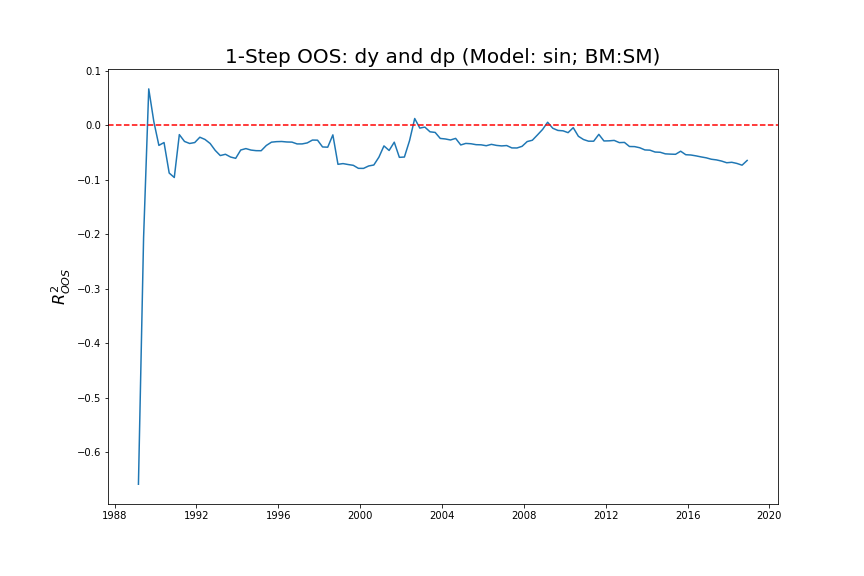
\includegraphics[width=0.9\linewidth]{OOS_plots/sin_co1_SM.png}
		\caption{co1}
	\end{subfigure}
	\begin{subfigure}[b]{0.42\linewidth}
		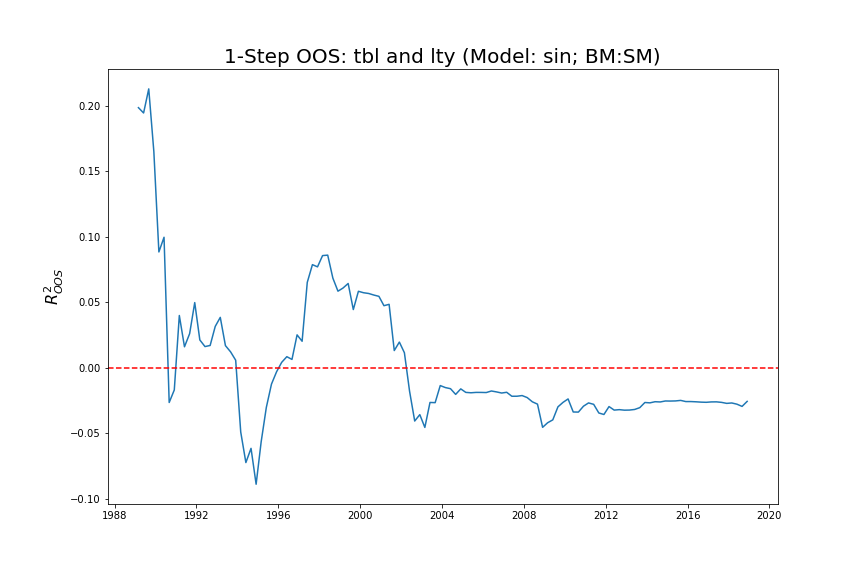
\includegraphics[width=0.9\linewidth]{OOS_plots/sin_co2_SM.png}
		\caption{co2}
	\end{subfigure}
	\begin{subfigure}[b]{0.42\linewidth}
		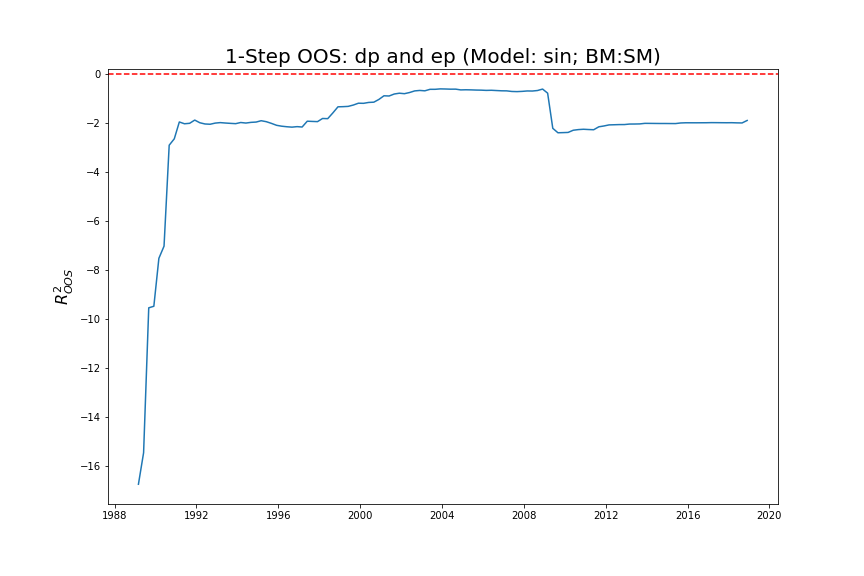
\includegraphics[width=0.9\linewidth]{OOS_plots/sin_co3_SM.png}
		\caption{co3}
	\end{subfigure}
	\begin{subfigure}[b]{0.42\linewidth}
		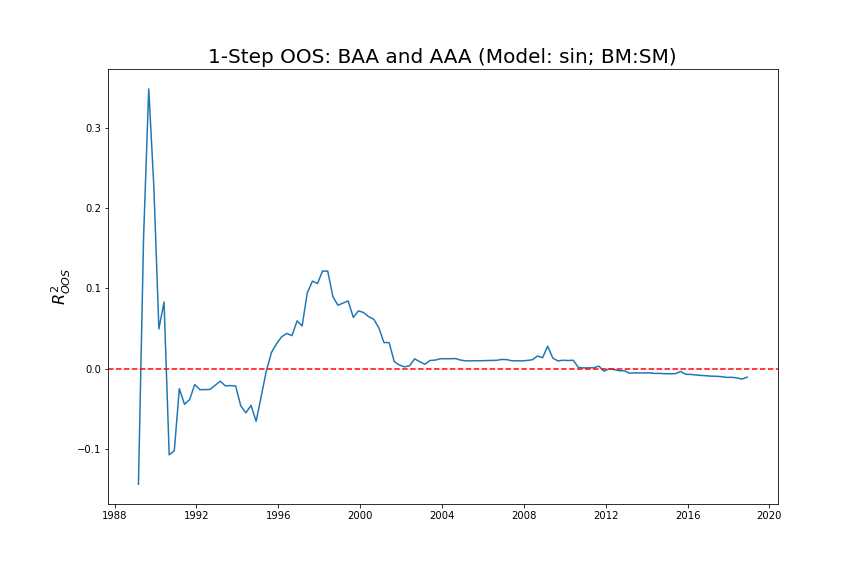
\includegraphics[width=0.9\linewidth]{OOS_plots/sin_co4_SM.png}
		\caption{co4}
	\end{subfigure}
	\label{g1}
\end{figure}

\begin{figure}[!htbp]
	\centering
	\caption{OOS Results for Model with $f_2$}
	\begin{subfigure}[b]{0.42\linewidth}
		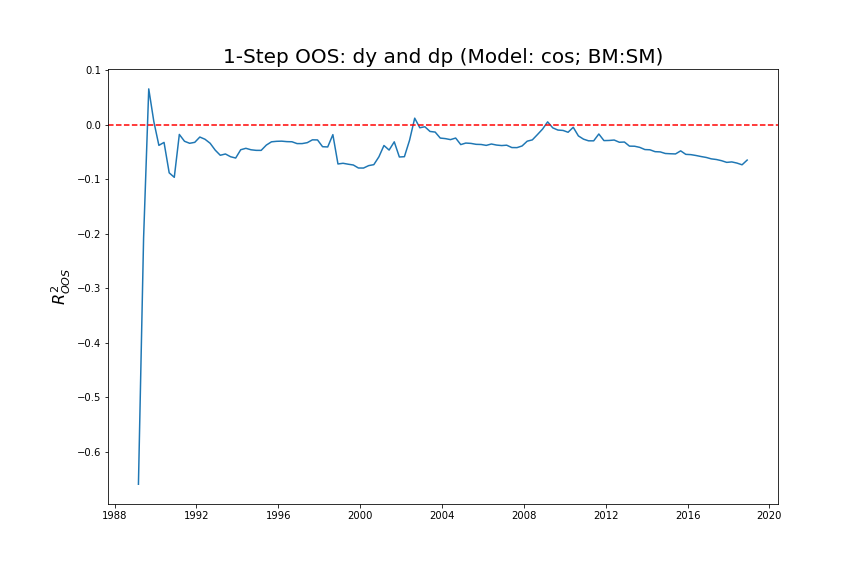
\includegraphics[width=0.9\linewidth]{OOS_plots/cos_co1_SM.png}
		\caption{co1}
	\end{subfigure}
	\begin{subfigure}[b]{0.42\linewidth}
		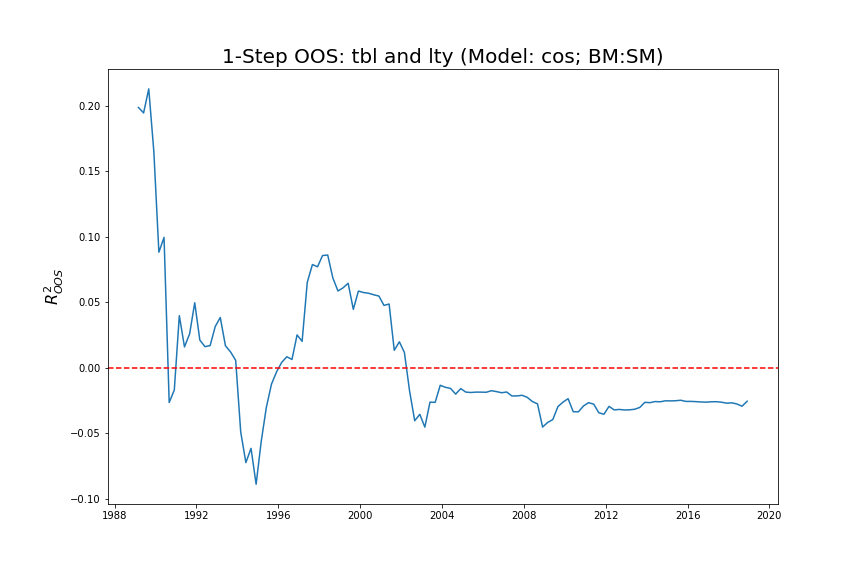
\includegraphics[width=0.9\linewidth]{OOS_plots/cos_co2_SM.png}
		\caption{co2}
	\end{subfigure}
	\begin{subfigure}[b]{0.42\linewidth}
		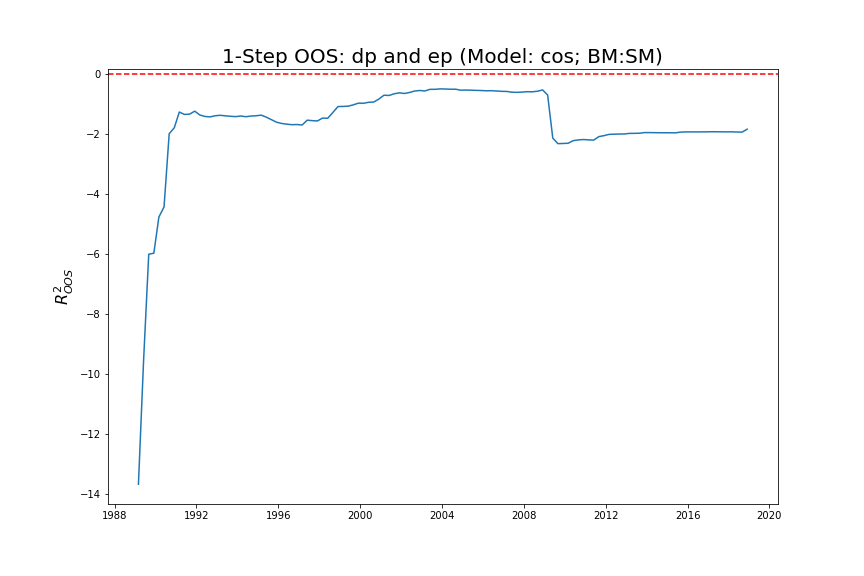
\includegraphics[width=0.9\linewidth]{OOS_plots/cos_co3_SM.png}
		\caption{co3}
	\end{subfigure}
	\begin{subfigure}[b]{0.42\linewidth}
		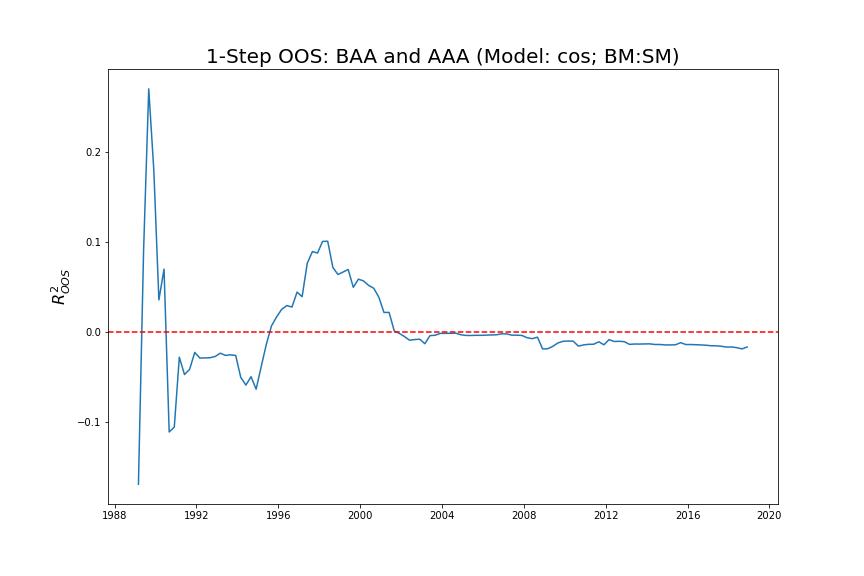
\includegraphics[width=0.9\linewidth]{OOS_plots/cos_co4_SM.png}
		\caption{co4}
	\end{subfigure}
	\label{g2}
\end{figure}

\begin{figure}[!htbp]
	\centering
	\caption{OOS Results for Model with $f_3$}
	\begin{subfigure}[b]{0.42\linewidth}
		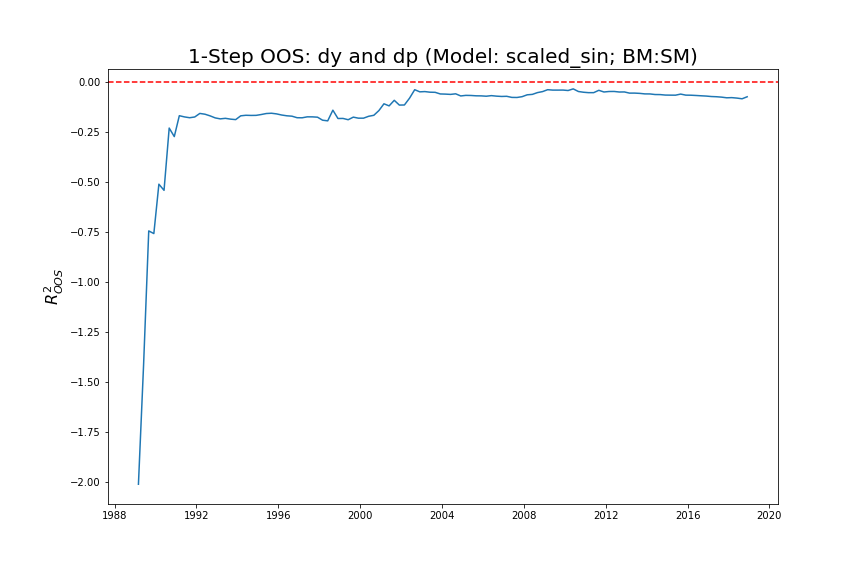
\includegraphics[width=0.9\linewidth]{OOS_plots/scaled_sin_co1_SM.png}
		\caption{co1}
	\end{subfigure}
	\begin{subfigure}[b]{0.42\linewidth}
		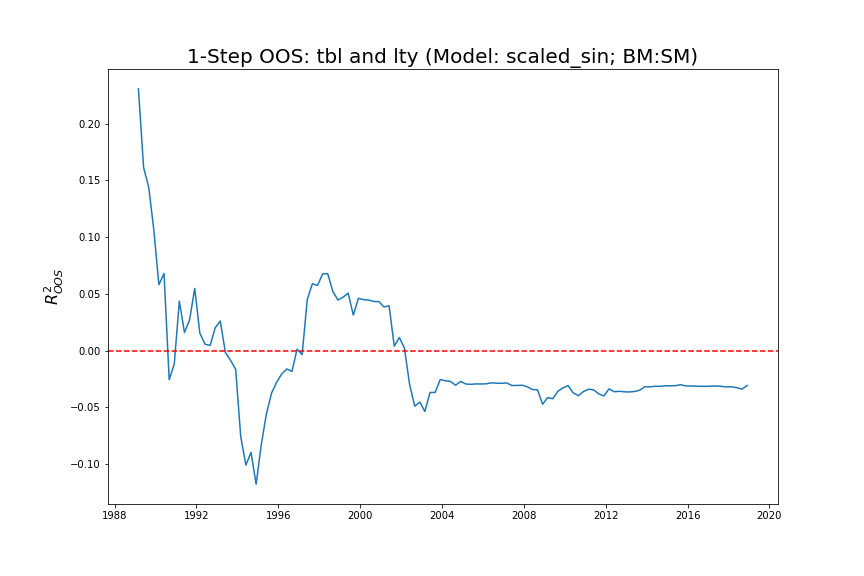
\includegraphics[width=0.9\linewidth]{OOS_plots/scaled_sin_co2_SM.png}
		\caption{co2}
	\end{subfigure}
	\begin{subfigure}[b]{0.42\linewidth}
		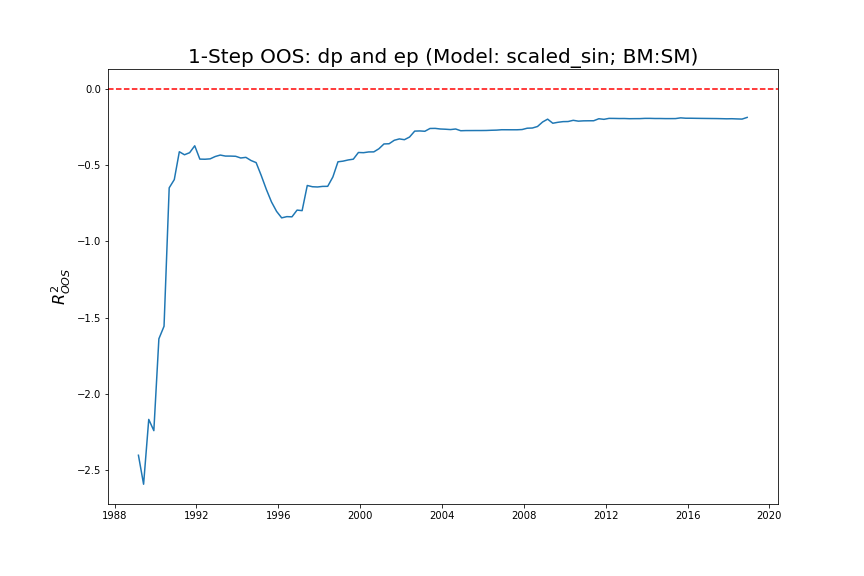
\includegraphics[width=0.9\linewidth]{OOS_plots/scaled_sin_co3_SM.png}
		\caption{co3}
	\end{subfigure}
	\begin{subfigure}[b]{0.42\linewidth}
		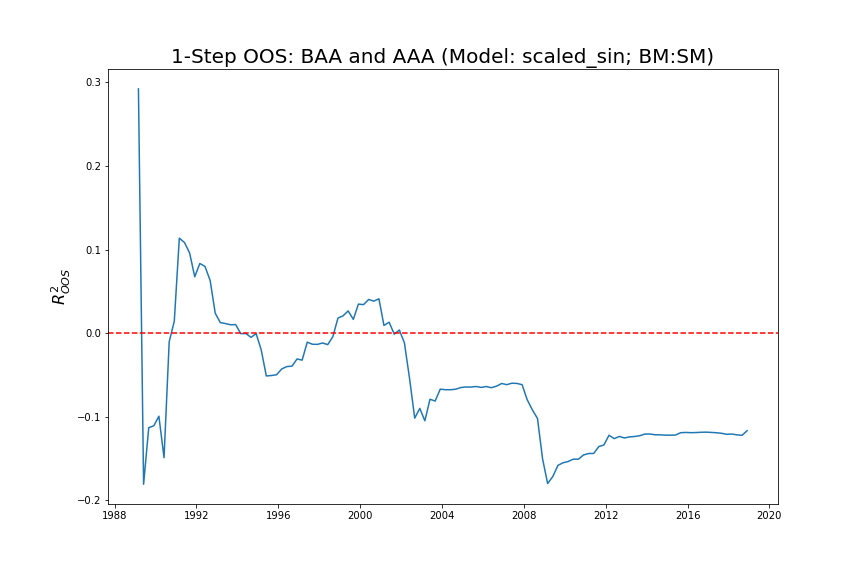
\includegraphics[width=0.9\linewidth]{OOS_plots/scaled_sin_co4_SM.png}
		\caption{co4}
	\end{subfigure}
	\label{g3}
\end{figure}

\begin{figure}[!htbp]
	\centering
	\caption{OOS Results for Model with $f_4$}
	\begin{subfigure}[b]{0.42\linewidth}
		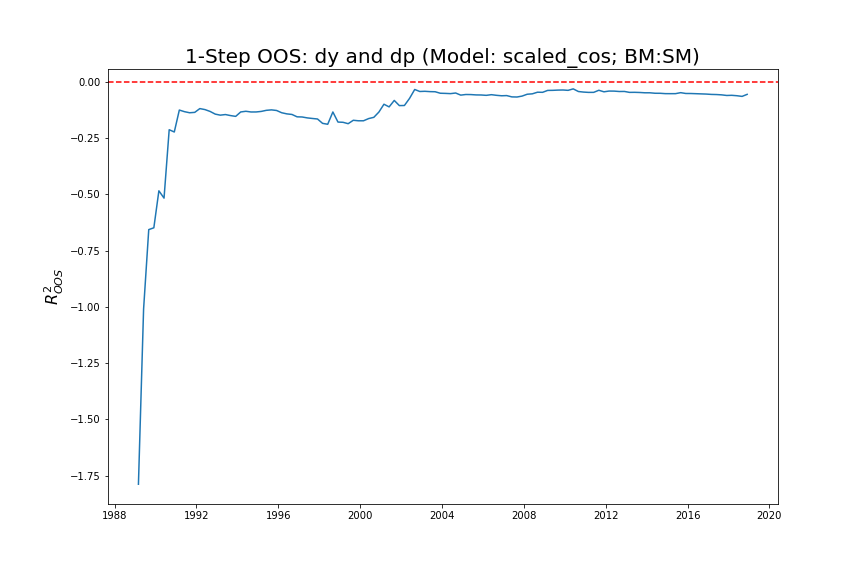
\includegraphics[width=0.9\linewidth]{OOS_plots/scaled_cos_co1_SM.png}
		\caption{co1}
	\end{subfigure}
	\begin{subfigure}[b]{0.42\linewidth}
		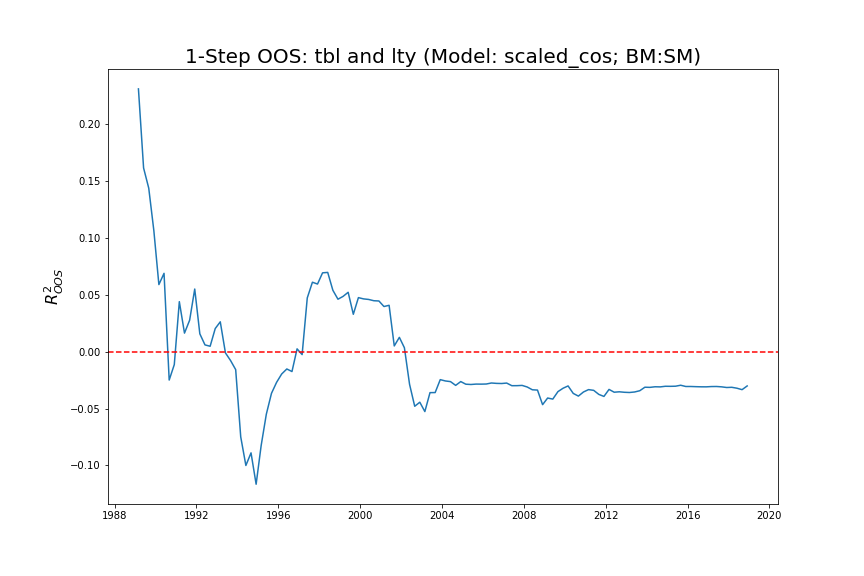
\includegraphics[width=0.9\linewidth]{OOS_plots/scaled_cos_co2_SM.png}
		\caption{co2}
	\end{subfigure}
	\begin{subfigure}[b]{0.42\linewidth}
		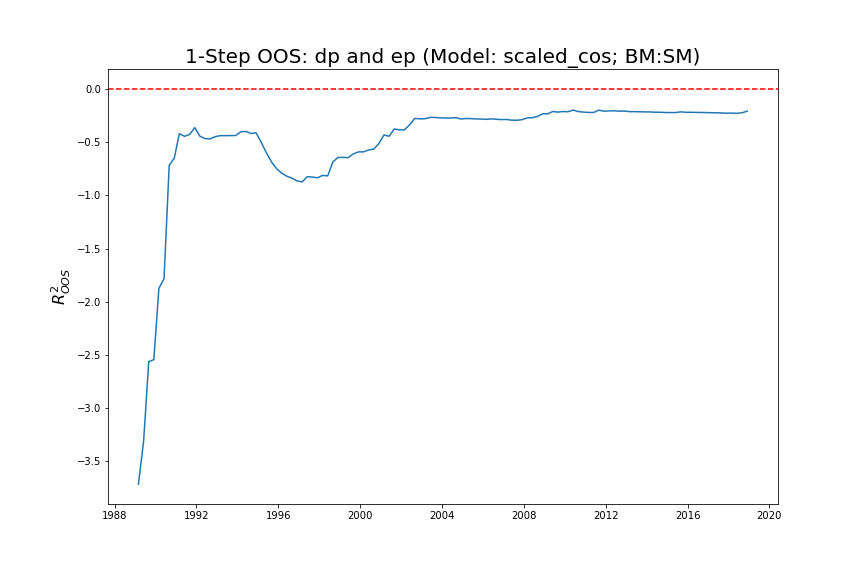
\includegraphics[width=0.9\linewidth]{OOS_plots/scaled_cos_co3_SM.png}
		\caption{co3}
	\end{subfigure}
	\begin{subfigure}[b]{0.42\linewidth}
		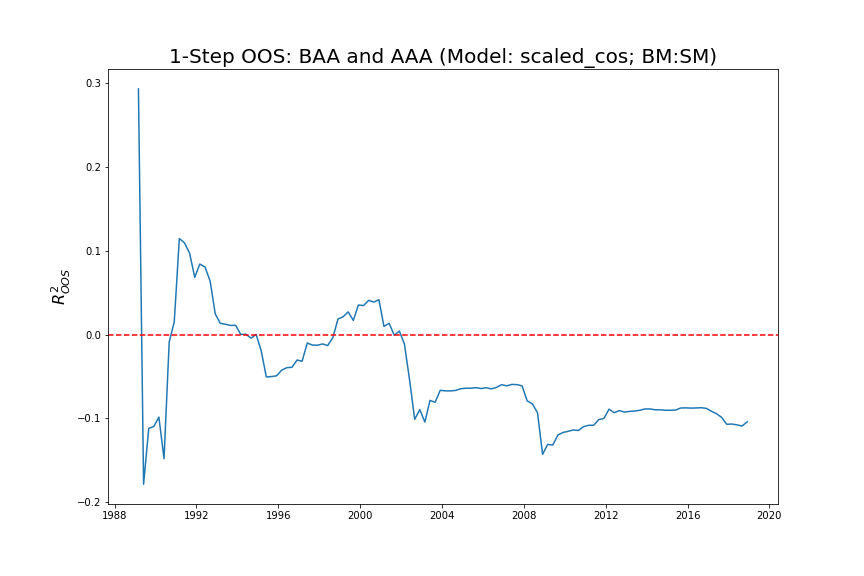
\includegraphics[width=0.9\linewidth]{OOS_plots/scaled_cos_co4_SM.png}
		\caption{co4}
	\end{subfigure}
	\label{g4}
\end{figure}


\begin{figure}[!htbp]
	\centering
	\caption{OOS Results for Model with $f_5$}
	\begin{subfigure}[b]{0.42\linewidth}
		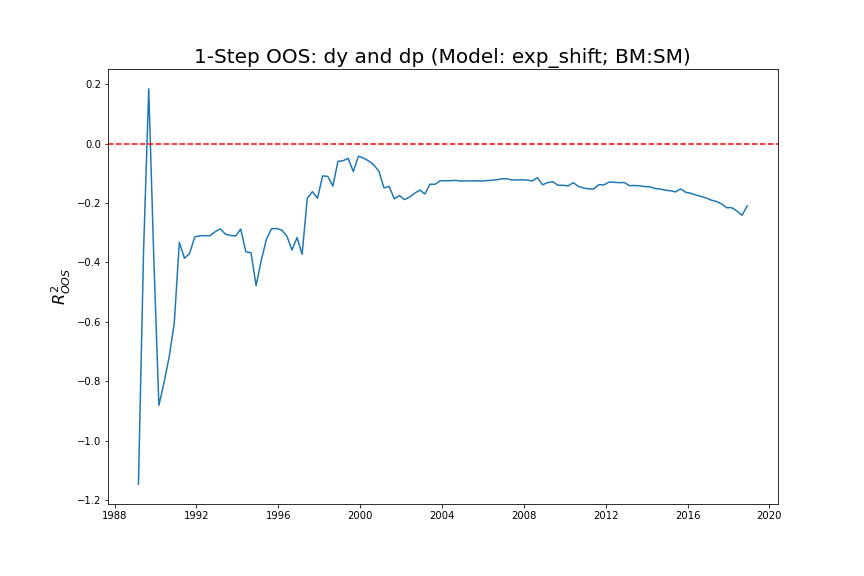
\includegraphics[width=0.9\linewidth]{OOS_plots/exp_shift_co1_SM.png}
		\caption{co1}
	\end{subfigure}
	\begin{subfigure}[b]{0.42\linewidth}
		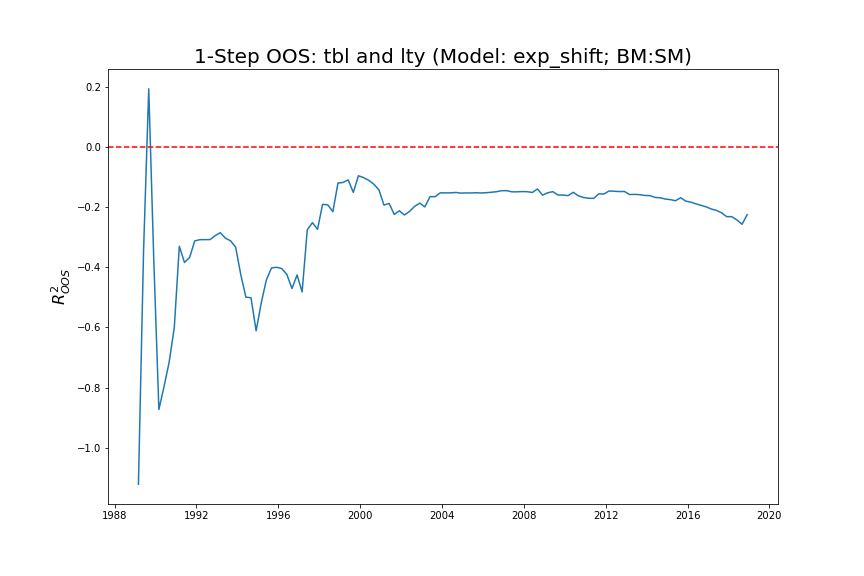
\includegraphics[width=0.9\linewidth]{OOS_plots/exp_shift_co2_SM.png}
		\caption{co2}
	\end{subfigure}
	\begin{subfigure}[b]{0.42\linewidth}
		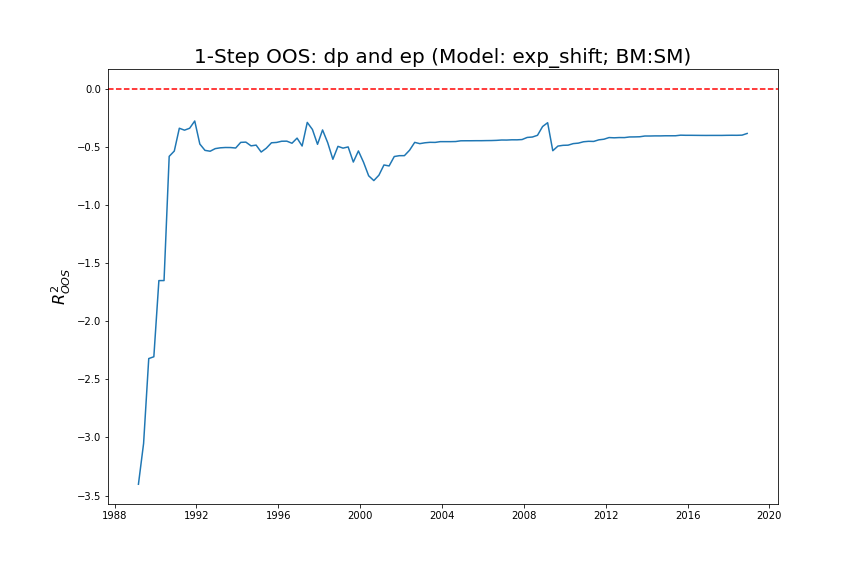
\includegraphics[width=0.9\linewidth]{OOS_plots/exp_shift_co3_SM.png}
		\caption{co3}
	\end{subfigure}
	\begin{subfigure}[b]{0.42\linewidth}
		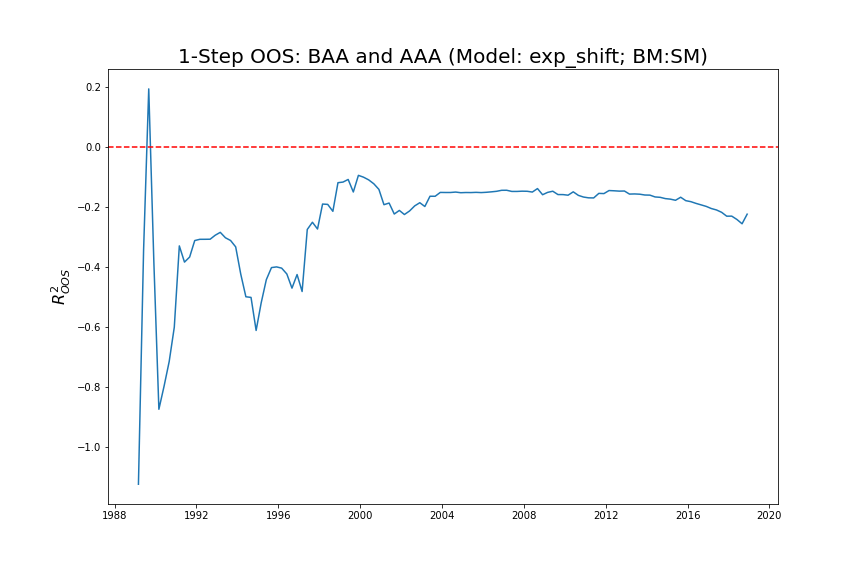
\includegraphics[width=0.9\linewidth]{OOS_plots/exp_shift_co4_SM.png}
		\caption{co4}
	\end{subfigure}
	\label{g5}
\end{figure}

\begin{figure}[!htbp]
	\centering
	\caption{OOS Results for Model with $f_6$}
	\begin{subfigure}[b]{0.42\linewidth}
		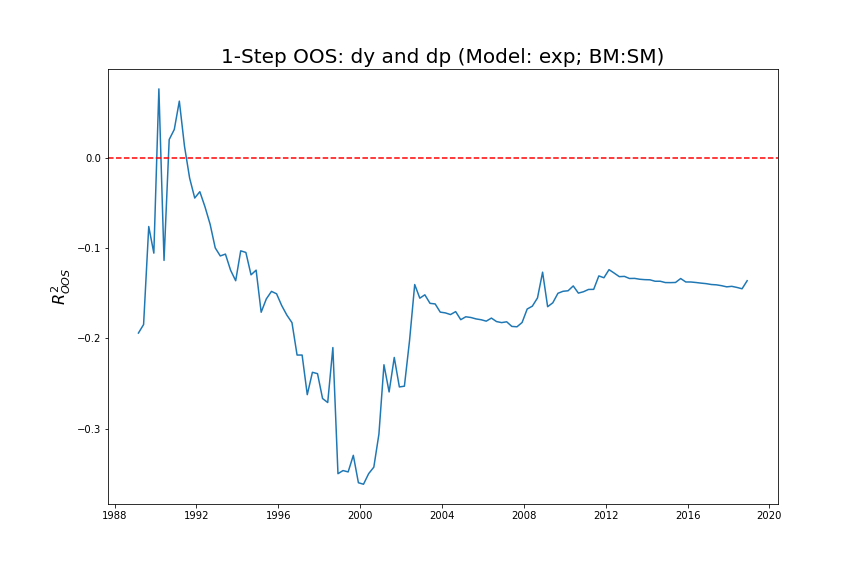
\includegraphics[width=0.9\linewidth]{OOS_plots/exp_co1_SM.png}
		\caption{co1}
	\end{subfigure}
	\begin{subfigure}[b]{0.42\linewidth}
		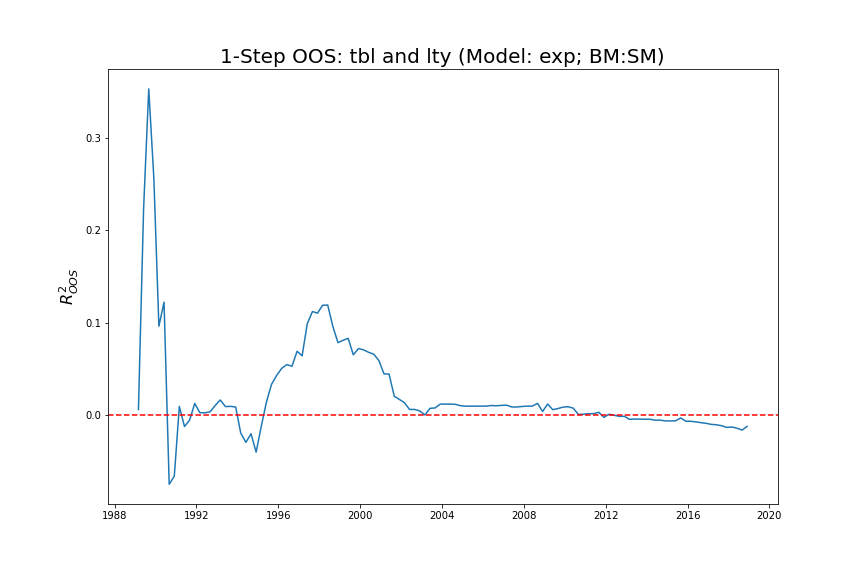
\includegraphics[width=0.9\linewidth]{OOS_plots/exp_co2_SM.png}
		\caption{co2}
	\end{subfigure}
	\begin{subfigure}[b]{0.42\linewidth}
		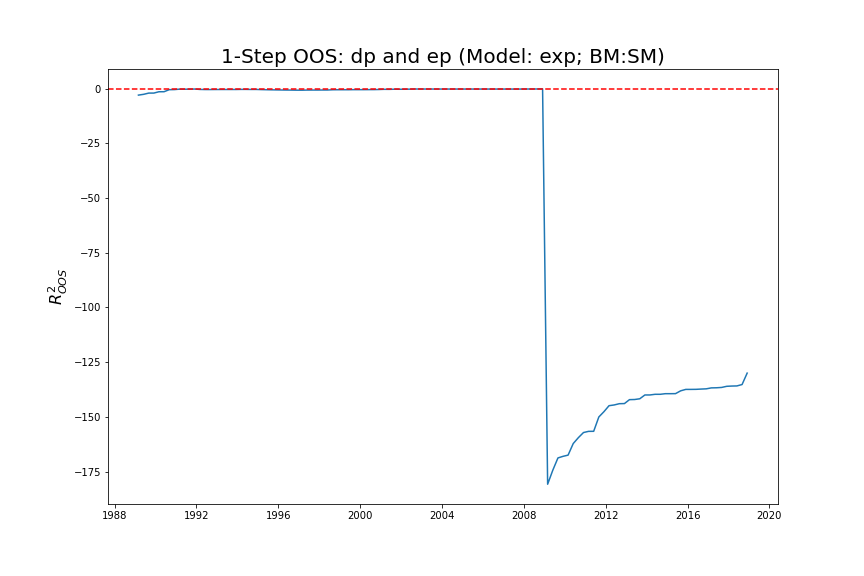
\includegraphics[width=0.9\linewidth]{OOS_plots/exp_co3_SM.png}
		\caption{co3}
	\end{subfigure}
	\begin{subfigure}[b]{0.42\linewidth}
		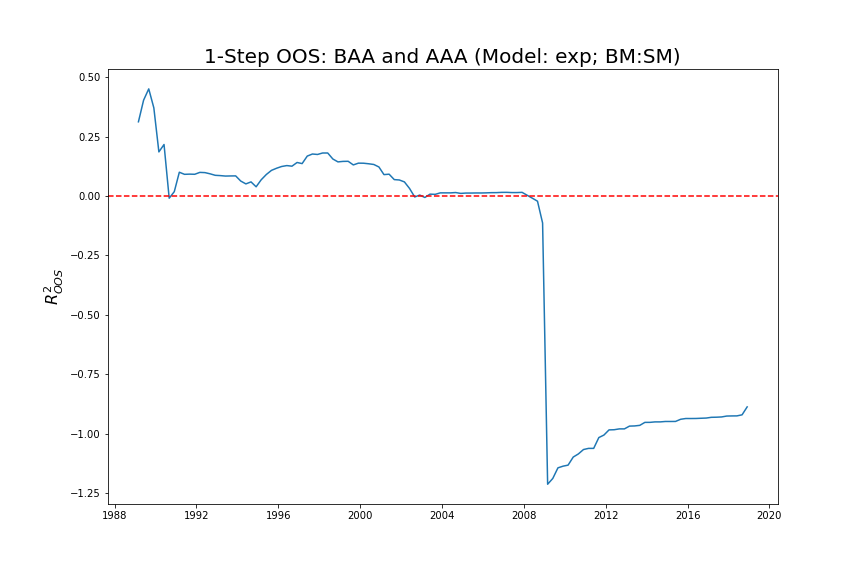
\includegraphics[width=0.9\linewidth]{OOS_plots/exp_co4_SM.png}
		\caption{co4}
	\end{subfigure}
	\label{g6}
\end{figure}


\begin{figure}[!htbp]
	\centering
	\caption{OOS Results for Model with $f_7$}
	\begin{subfigure}[b]{0.42\linewidth}
		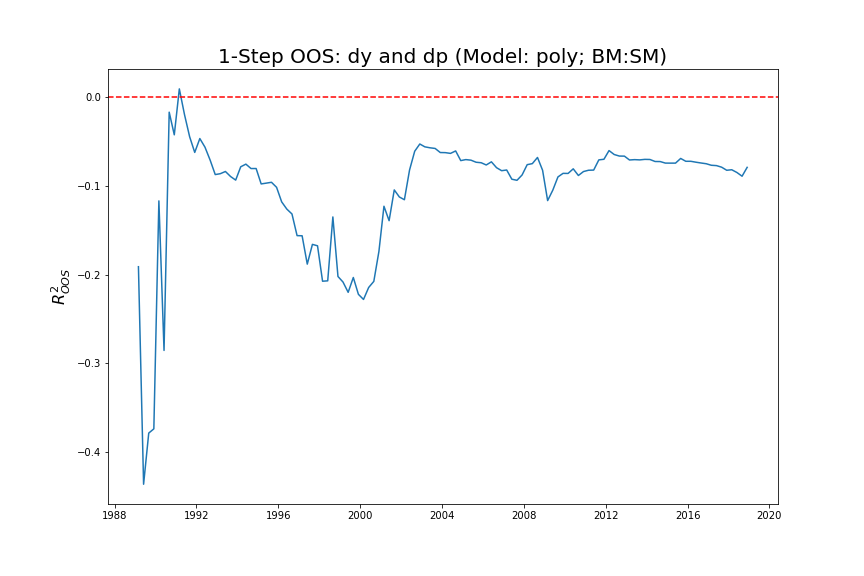
\includegraphics[width=0.9\linewidth]{OOS_plots/poly_co1_SM.png}
		\caption{co1}
	\end{subfigure}
	\begin{subfigure}[b]{0.42\linewidth}
		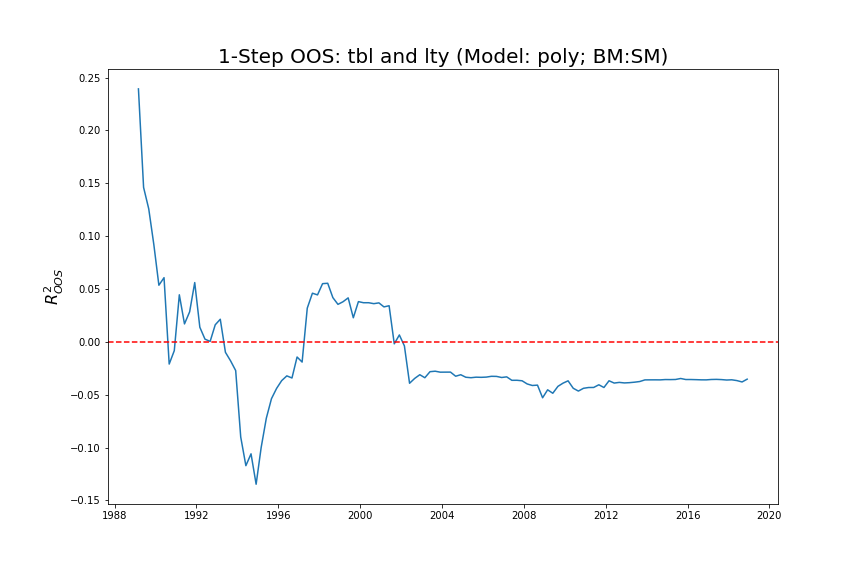
\includegraphics[width=0.9\linewidth]{OOS_plots/poly_co2_SM.png}
		\caption{co2}
	\end{subfigure}
	\begin{subfigure}[b]{0.42\linewidth}
		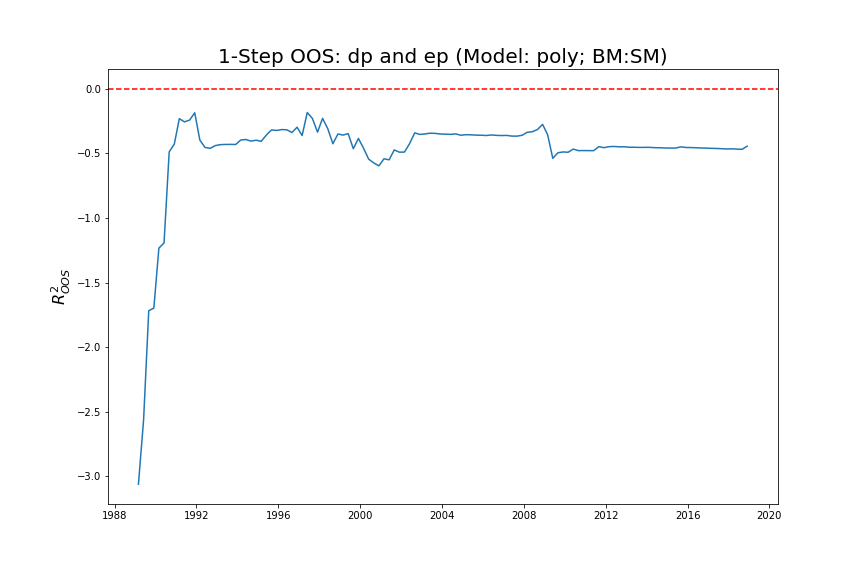
\includegraphics[width=0.9\linewidth]{OOS_plots/poly_co3_SM.png}
		\caption{co3}
	\end{subfigure}
	\begin{subfigure}[b]{0.42\linewidth}
		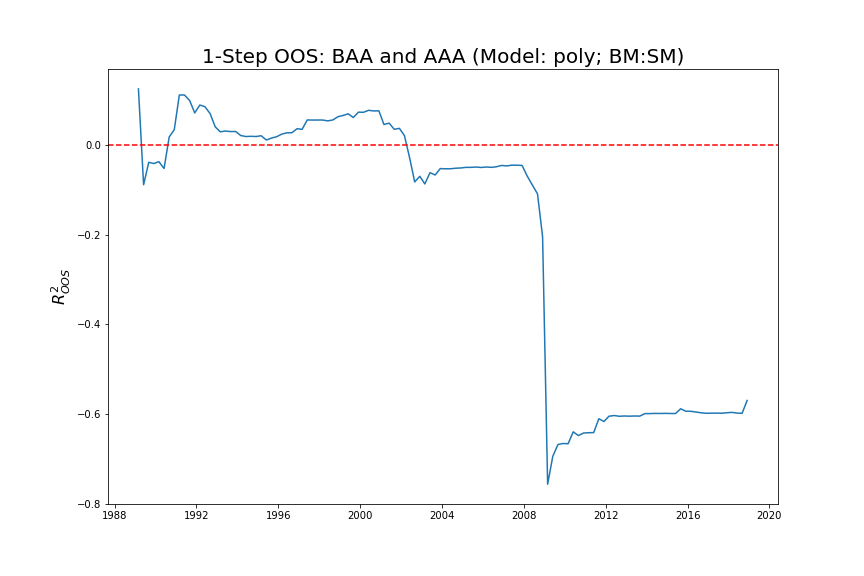
\includegraphics[width=0.9\linewidth]{OOS_plots/poly_co4_SM.png}
		\caption{co4}
	\end{subfigure}
	\label{g7}
\end{figure}

\begin{figure}[!htbp]
	\centering
	\caption{OOS Results for Model with $g_8$}
	\begin{subfigure}[b]{0.42\linewidth}
		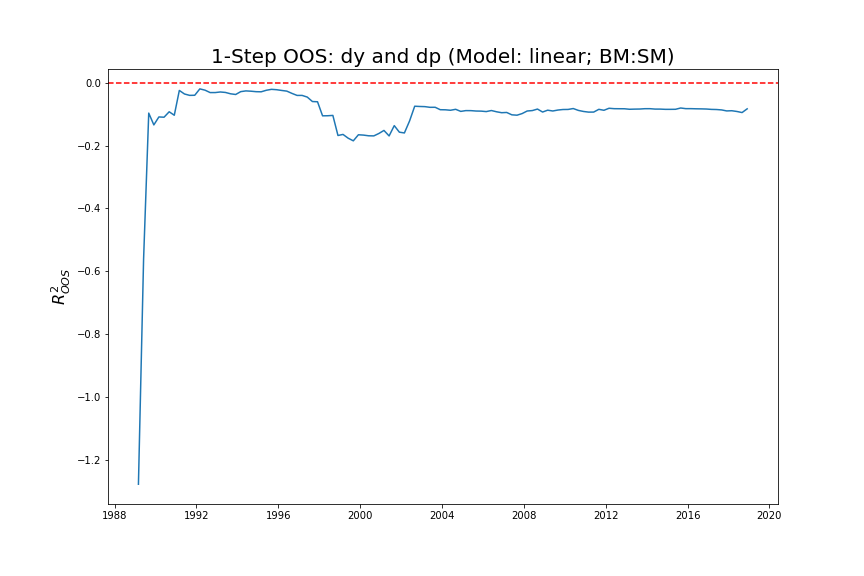
\includegraphics[width=0.9\linewidth]{OOS_plots/linear_co1_SM.png}
		\caption{co1}
	\end{subfigure}
	\begin{subfigure}[b]{0.42\linewidth}
		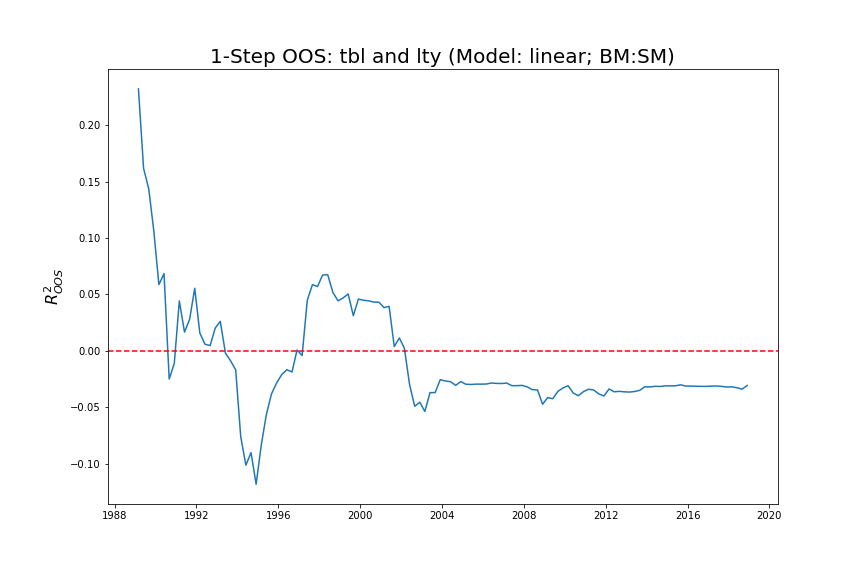
\includegraphics[width=0.9\linewidth]{OOS_plots/linear_co2_SM.png}
		\caption{co2}
	\end{subfigure}
	\begin{subfigure}[b]{0.42\linewidth}
		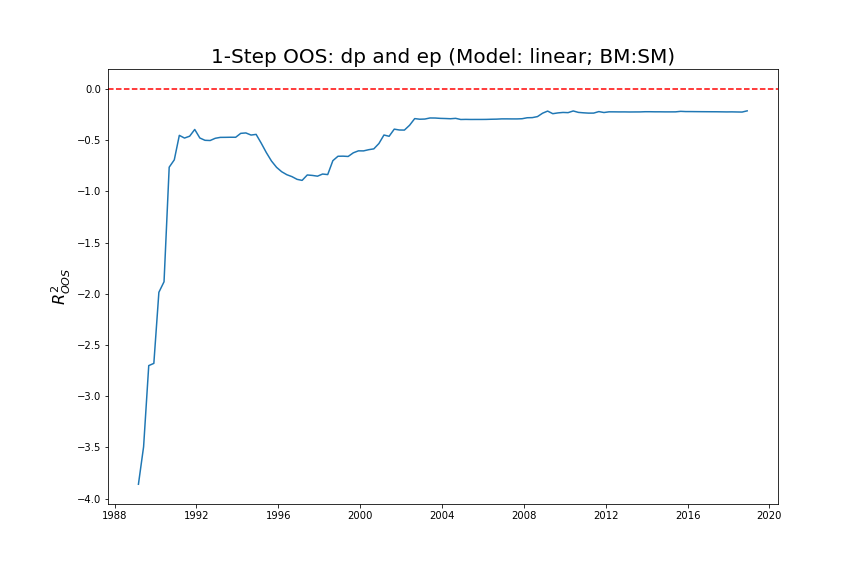
\includegraphics[width=0.9\linewidth]{OOS_plots/linear_co3_SM.png}
		\caption{co3}
	\end{subfigure}
	\begin{subfigure}[b]{0.42\linewidth}
		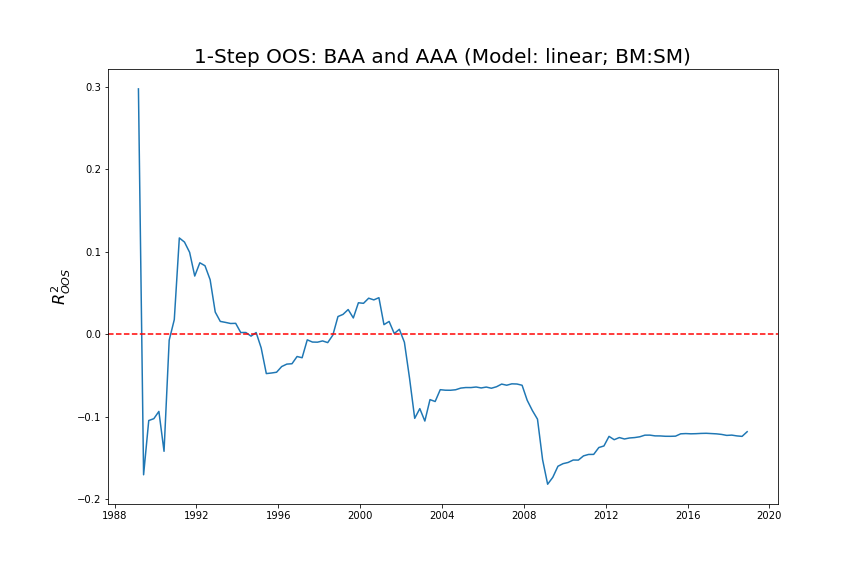
\includegraphics[width=0.9\linewidth]{OOS_plots/linear_co4_SM.png}
		\caption{co4}
	\end{subfigure}
	\label{g8}
\end{figure}
\pagebreak

To compare the performances of the 8 functional forms with the 4 different variable combinations, we calculate the percentage of positive $R^2_{OOS}$ in the forecasting period. The results are shown in table (\ref{perct}). It is clear that for combination co3 (dp and ep), none of the functions can perform better than sample mean prediction. However, for combinations co2 and co4, for more than half of out-of-sample period, $g_1$ and $g_6$ can outperform sample mean. And other functional forms also can provide positive results. 

% Table generated by Excel2LaTeX from sheet 'Sheet1'
\begin{table}[htbp]
  \centering
  \caption{Percentage of Positive $R^2_{OOS}$}
    \begin{tabular}{ccccccccc}
    \toprule
          & $g_1$    & $g_2$    & $g_3$    & $g_4$    & $g_5$    & $g_6$    & $g_7$    & $g_8$ \\
    \midrule
    co1   & 3.23\% & 3.23\% & 0.00\% & 0.00\% & 2.42\% & 7.26\% & 4.03\% & 0.00\% \\
    co2   & 37.90\% & 37.90\% & 32.26\% & 32.26\% & 2.42\% & \textcolor[rgb]{ .753,  0,  0}{68.55\%} & 29.84\% & 32.26\% \\
    co3   & 0.00\% & 0.00\% & 0.00\% & 0.00\% & 0.00\% & 0.00\% & 0.00\% & 0.00\% \\
    co4   & \textcolor[rgb]{ .753,  0,  0}{57.26\%} & 24.19\% & 24.19\% & 26.61\% & 2.42\% & \textcolor[rgb]{ .753,  0,  0}{62.90\%} & 41.94\% & 27.42\% \\
    \bottomrule
    \bottomrule
    \end{tabular}%
  \label{perct}%
\end{table}%

To conclude, no matter which function we use, combinations co2 and co4 tend to have better results than other variable pairs. And among the 8 functions, $g_6$ is the best for all the 4 combinations in terms of the percentage of positive $R^2_{OOS}$. The two trigonometric functions also provide good OOS results, especially for $g_1$ and co4. But considering the scale parameter in $g_3$ and $g_4$ does not improve the forecast. For polynomial function, it can outperform sample mean except for combination co3, although it is not as good as other functional forms.

\subsubsection{OOS Performance v.s. Other Benchmark Models}
For another commonly used time series model, the AR(1) model, we can also see from the figur \ref{vsAR1} that the partially nonlinear models can perform better. When using model containing the nonlinear functional form $f_1$ and variable combination $co2$, our partially nonlinear model can outperform AR(1) model for most of the period before 2006. Similar for the model with functional form $f_5$, our model performs better when using co2 before 2012.


\begin{figure}[!htbp]
	\centering
	\caption{OOS Performance (Benchmark: AR(1) Model)}
	\begin{subfigure}[b]{0.42\linewidth}
		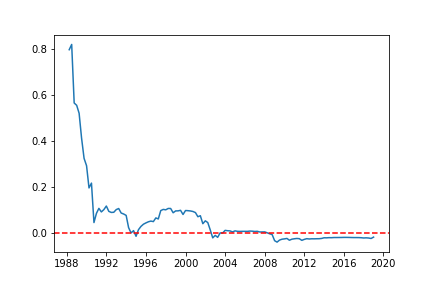
\includegraphics[width=1.2\linewidth]{plots/co2_AR1_g1.png}
		\caption{co2 model containing $f_1$}
	\end{subfigure}
	\begin{subfigure}[b]{0.42\linewidth}
		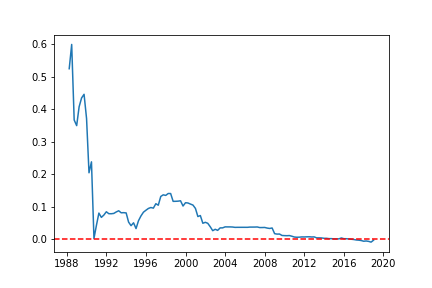
\includegraphics[width=1.2\linewidth]{plots/co2_AR1_g5.png}
		\caption{co2 model containing $f_5$}
	\end{subfigure}
	\label{vsAR1}
\end{figure}

Figure \ref{vsNL} presents the $R^2_{OOS}$ when using the nonlinear models in chapter 2 as the benchmark model. In the nonlinear model, we did not include the stationary variables but we considered the same nonlinear functional forms. 

From the figure, we can see that when using variable combination co2 and function with nonlinear form $f_1$, the partially nonlinear model can outperform the nonlinear model during the whole out-of-sample period. And for the variable combination co4, when using function containing nonlinear part $f_7$, the partially nonlinear model outperforms the nonlinear model before 2009. 

\begin{figure}[!htbp]
	\centering
	\caption{OOS Performance (Benchmark: Nonlinear Model)}
	\begin{subfigure}[b]{0.42\linewidth}
		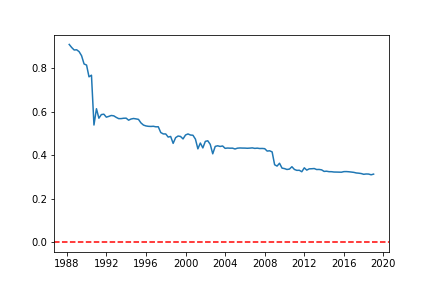
\includegraphics[width=1.2\linewidth]{plots/co1_NLS_g1.png}
		\caption{co1 using model containing $f_1$}
	\end{subfigure}
	\begin{subfigure}[b]{0.42\linewidth}
		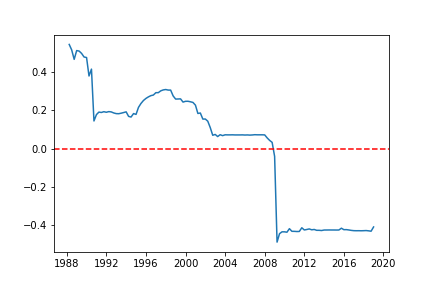
\includegraphics[width=1.2\linewidth]{plots/co4_NLS_g7.png}
		\caption{co4 using model containing $f_7$}
	\end{subfigure}
	\label{vsNL}
\end{figure}

When compared with the AR(2) models, the partially nonlinear models also provide a good out-of-sample performance. The model with nonlinear part $f_3$ outperforms the AR(2) model before 2009 when using variable combination co4.

And for the model with nonlinear component $f_5$, it outperforms the AR(2) model during the whole out-of-sample period (for variable combination co2). 

\begin{figure}[!htbp]
	\centering
	\caption{OOS Performance (Benchmark: AR(2) Models)}
	\begin{subfigure}[b]{0.42\linewidth}
		\includegraphics[width=1.2\linewidth]{plots/co4_AR2_g3.png}
		\caption{co4 using model containing $f_3$}
	\end{subfigure}
	\begin{subfigure}[b]{0.42\linewidth}
		\includegraphics[width=1.2\linewidth]{plots/co2_AR2_g5.png}
		\caption{co2 using model containing $f_5$}
	\end{subfigure}
	\label{vsNL}
\end{figure}

Therefore, we can conclude that the partially nonlinear models can outperform most of the commonly used time series models. And by including the stationary vairiables $y_{t-1}$ and the "cay" variable, our partially nonlinear models tend to show a much better out-of-sample performance.

\section{conclusion}
In this chapter, we consider a partially nonlinear single-index model, which allows for lagged dependent variables, stationary variables, cointegrated and non-cointegrated variables. We propose a three-step estimation method to estimate the model and includes a constraint on $\theta$ (the coefficient for the non-stationary variables) and a truncation condition on $x_t$. 

From the simulation results, we can see that the estimators have good finite sample properties and good convergence. We also find that the constraint provides finite sample gains for the CLS estimators. In addition, we also find that when using cointegrated $x_t$, both the NLS and CLS estimators have a better performance. And among the 7 functional forms we consider, the model with polynomial functional form  gives the best simulation performance. 

Based on the simulation results, we focus on cointegrated variables and the constrained nonlinear least square method in the empirical study. We apply the model to the \cite{welch2008comprehensive} dataset and investigate the predictability using co-integrated variable combinations. We find that the partially nonlinear models can outperform sample mean model both in-sample and out-of-sample. When using other benchmark models, such as AR(1) model and AR(2) model, our models also provides better in-sample performance for certain variable combinations and nonlinear functional forms. In terms of out-of-sample, our models outperforms the two time series models in a consecutive period. 

And by including lagged dependent variable and the stationary "cay" variable, the partially nonlinear models give better out-of-sample forecast than the nonlinear models over a consecutive period. Therefore, we can conclude that by considering nonlinearities and auto-correlation in the dependent variable, we can achieve out-of-sample forecasting gains.


%\begin{figure}[!htbp]
%	\centering
%	\caption{OOS Results for dp and dy, Taylor-initials}
%	\begin{subfigure}[b]{0.42\linewidth}
%		\includegraphics[width=1.2\linewidth]{OOS_plots/sin_co1_SM.png}
%		%		\caption{ Intercept}
%	\end{subfigure}
%	\begin{subfigure}[b]{0.42\linewidth}
%		\includegraphics[width=1.2\linewidth]{OOS_plots/cos_co1_SM.png}
%		%		\caption{ Intercept}
%	\end{subfigure}
%	\begin{subfigure}[b]{0.42\linewidth}
%		\includegraphics[width=1.2\linewidth]{OOS_plots/scaled_sin_co1_SM.png}
%		%		\caption{ Intercept}	\end{subfigure}
%	\end{subfigure}
%	\begin{subfigure}[b]{0.42\linewidth}
%		\includegraphics[width=1.2\linewidth]{OOS_plots/scaled_cos_co1_SM.png}
%		%		\caption{ Intercept}
%	\end{subfigure}
%	\begin{subfigure}[b]{0.42\linewidth}
%		\includegraphics[width=1.2\linewidth]{OOS_plots/exp_co1_SM.png}
%		%		\caption{ Intercept}
%	\end{subfigure}
%	\begin{subfigure}[b]{0.42\linewidth}
%		\includegraphics[width=1.2\linewidth]{OOS_plots/exp_shift_co1_SM.png}
%		%		\caption{ Intercept}
%	\end{subfigure}
%	\begin{subfigure}[b]{0.42\linewidth}
%		\includegraphics[width=1.2\linewidth]{OOS_plots/poly_co1_SM.png}
%		%		\caption{ Intercept}
%	\end{subfigure}
%	\begin{subfigure}[b]{0.42\linewidth}
%		\includegraphics[width=1.2\linewidth]{OOS_plots/linear_co1_SM.png}
%		%		\caption{ Intercept}
%	\end{subfigure}
%\end{figure}
%
%\begin{figure}[!htbp]
%	\centering
%	\caption{OOS Results for tbl and lty, Taylor-initials}
%	\begin{subfigure}[b]{0.42\linewidth}
%		\includegraphics[width=1.2\linewidth]{OOS_plots/sin_co2_SM.png}
%		%		\caption{ Intercept}
%	\end{subfigure}
%	\begin{subfigure}[b]{0.42\linewidth}
%		\includegraphics[width=1.2\linewidth]{OOS_plots/cos_co2_SM.png}
%		%		\caption{ Intercept}
%	\end{subfigure}
%	\begin{subfigure}[b]{0.42\linewidth}
%		\includegraphics[width=1.2\linewidth]{OOS_plots/scaled_sin_co2_SM.png}
%		%		\caption{ Intercept}	\end{subfigure}
%	\end{subfigure}
%	\begin{subfigure}[b]{0.42\linewidth}
%		\includegraphics[width=1.2\linewidth]{OOS_plots/scaled_cos_co2_SM.png}
%		%		\caption{ Intercept}
%	\end{subfigure}
%	\begin{subfigure}[b]{0.42\linewidth}
%		\includegraphics[width=1.2\linewidth]{OOS_plots/exp_co2_SM.png}
%		%		\caption{ Intercept}
%	\end{subfigure}
%	\begin{subfigure}[b]{0.42\linewidth}
%		\includegraphics[width=1.2\linewidth]{OOS_plots/exp_shift_co2_SM.png}
%		%		\caption{ Intercept}
%	\end{subfigure}
%	\begin{subfigure}[b]{0.42\linewidth}
%		\includegraphics[width=1.2\linewidth]{OOS_plots/poly_co2_SM.png}
%		%		\caption{ Intercept}
%	\end{subfigure}
%	\begin{subfigure}[b]{0.42\linewidth}
%		\includegraphics[width=1.2\linewidth]{OOS_plots/linear_co2_SM.png}
%		%		\caption{ Intercept}
%	\end{subfigure}
%	\label{co2}
%\end{figure}
%\pagebreak
%
%%\subsection{OOS Results for dp and ep}
%\begin{figure}[!htbp]
%	\centering
%	\caption{OOS Results for dp and ep, Taylor-initials}
%	\begin{subfigure}[b]{0.42\linewidth}
%		\includegraphics[width=1.2\linewidth]{OOS_plots/sin_co3_SM.png}
%		%		\caption{ Intercept}
%	\end{subfigure}
%	\begin{subfigure}[b]{0.42\linewidth}
%		\includegraphics[width=1.2\linewidth]{OOS_plots/cos_co3_SM.png}
%		%		\caption{ Intercept}
%	\end{subfigure}
%	\begin{subfigure}[b]{0.42\linewidth}
%		\includegraphics[width=1.2\linewidth]{OOS_plots/scaled_sin_co3_SM.png}
%		%		\caption{ Intercept}	\end{subfigure}
%	\end{subfigure}
%	\begin{subfigure}[b]{0.42\linewidth}
%		\includegraphics[width=1.2\linewidth]{OOS_plots/scaled_cos_co3_SM.png}
%		%		\caption{ Intercept}
%	\end{subfigure}
%	\begin{subfigure}[b]{0.42\linewidth}
%		\includegraphics[width=1.2\linewidth]{OOS_plots/exp_co3_SM.png}
%		%		\caption{ Intercept}
%	\end{subfigure}
%	\begin{subfigure}[b]{0.42\linewidth}
%		\includegraphics[width=1.2\linewidth]{OOS_plots/exp_shift_co3_SM.png}
%		%		\caption{ Intercept}
%	\end{subfigure}
%	\begin{subfigure}[b]{0.42\linewidth}
%		\includegraphics[width=1.2\linewidth]{OOS_plots/poly_co3_SM.png}
%		%		\caption{ Intercept}
%	\end{subfigure}
%	\begin{subfigure}[b]{0.42\linewidth}
%		\includegraphics[width=1.2\linewidth]{OOS_plots/linear_co3_SM.png}
%		%		\caption{ Intercept}
%	\end{subfigure}
%	\label{co3}
%\end{figure}
%\pagebreak
%
%%\subsection{OOS Results for BAA and AAA}
%\begin{figure}[!htbp]
%	\centering
%	\caption{OOS Results for BAA and AAA, Taylor-initials}
%	\begin{subfigure}[b]{0.42\linewidth}
%		\includegraphics[width=1.2\linewidth]{OOS_plots/sin_co4_SM.png}
%		%		\caption{ Intercept}
%	\end{subfigure}
%	\begin{subfigure}[b]{0.42\linewidth}
%		\includegraphics[width=1.2\linewidth]{OOS_plots/cos_co4_SM.png}
%		%		\caption{ Intercept}
%	\end{subfigure}
%	\begin{subfigure}[b]{0.42\linewidth}
%		\includegraphics[width=1.2\linewidth]{OOS_plots/scaled_sin_co4_SM.png}
%		%		\caption{ Intercept}	\end{subfigure}
%	\end{subfigure}
%	\begin{subfigure}[b]{0.42\linewidth}
%		\includegraphics[width=1.2\linewidth]{OOS_plots/scaled_cos_co4_SM.png}
%		%		\caption{ Intercept}
%	\end{subfigure}
%	\begin{subfigure}[b]{0.42\linewidth}
%		\includegraphics[width=1.2\linewidth]{OOS_plots/exp_co4_SM.png}
%		%		\caption{ Intercept}
%	\end{subfigure}
%	\begin{subfigure}[b]{0.42\linewidth}
%		\includegraphics[width=1.2\linewidth]{OOS_plots/exp_shift_co4_SM.png}
%		%		\caption{ Intercept}
%	\end{subfigure}
%	\begin{subfigure}[b]{0.42\linewidth}
%		\includegraphics[width=1.2\linewidth]{OOS_plots/poly_co4_SM.png}
%		%		\caption{ Intercept}
%	\end{subfigure}
%	\begin{subfigure}[b]{0.42\linewidth}
%		\includegraphics[width=1.2\linewidth]{OOS_plots/linear_co2_SM.png}
%		%		\caption{ Intercept}
%	\end{subfigure}
%	\label{co4}
%\end{figure}

% We can see that when using combination co1 (dp and dy), the trigonometric functions and the two exponential functions give better results than sample mean benchmark in the beginning of the forecasting period.For co2 (tbl and lty) and co4 (BAA and AAA-rated bonds), all functional forms except for the exponential function perform better than the benchmark in most of the periods before 2008. However, for co3 (dp and ep), we did not find a functional form that can deliver positive results.


\pagebreak

{\footnotesize
	
	\bibliographystyle{agsm}
	\bibliography{reference}
	
}
\pagebreak

\appendix
\section{In-sample Estimation Results}
% Table generated by Excel2LaTeX from sheet 'Sheet1'
\begin{table}[htbp]
	\centering
	\caption{Full-sample Estimation Results Using Taylor Initials}
	\begin{adjustbox}{max width=0.7\textwidth}
		\begin{tabular}{ccrrrrrrr}
			\toprule
			&       & \multicolumn{1}{c}{\textbf{$\theta_{1}$}} & \multicolumn{1}{c}{\textbf{$\theta_{2}$}} & \multicolumn{1}{c}{\textbf{$\beta_1$}} & \multicolumn{1}{c}{\textbf{$\beta_2$}} & \multicolumn{3}{c}{\textbf{$\gamma$}} \\
			\multirow{4}[0]{*}{\textbf{sin\_func}} & \textbf{co1} & -0.699 & 0.715 & -0.600 & 0.424 & 0.257 &       &  \\
			& \textbf{co2} & -0.775 & 0.632 & 0.064 & 0.399 & 0.185 &       &  \\
			& \textbf{co3} & -0.953 & 0.302 & 0.048 & 2.130 & -1.011 &       &  \\
			& \textbf{co4} & -0.742 & 0.670 & 0.081 & 0.474 & 0.236 &       &  \\
			\multirow{4}[0]{*}{\textbf{cos\_func}} & \textbf{co1} & -0.699 & 0.715 & -0.600 & 0.424 & -1.314 &       &  \\
			& \textbf{co2} & -0.775 & 0.632 & 0.063 & 0.398 & 30.030 &       &  \\
			& \textbf{co3} & -0.953 & 0.302 & 0.048 & 2.130 & -2.582 &       &  \\
			& \textbf{co4} & -0.743 & 0.670 & 0.081 & 0.474 & 187.161 &       &  \\
			\multirow{4}[0]{*}{\textbf{scaled\_sin\_func}} & \textbf{co1} & 0.678 & -0.735 & -0.139 & 0.476 & 9.132 & 0.333 &  \\
			& \textbf{co2} & -0.839 & 0.544 & 0.069 & 0.442 & 0.212 & 0.615 &  \\
			& \textbf{co3} & -0.947 & 0.320 & 0.100 & 0.508 & 0.313 & -0.030 &  \\
			& \textbf{co4} & 0.654 & -0.756 & 0.080 & 0.624 & 0.295 & 4.164 &  \\
			\multirow{4}[0]{*}{\textbf{scaled\_cos\_func}} & \textbf{co1} & -0.785 & 0.619 & 0.182 & 0.515 & 1.247 & 0.137 &  \\
			& \textbf{co2} & -0.843 & 0.538 & 0.069 & 0.442 & -1.359 & 0.610 &  \\
			& \textbf{co3} & -0.932 & 0.361 & 0.099 & 0.507 & 1.261 & 0.031 &  \\
			& \textbf{co4} & -0.654 & 0.756 & 0.080 & 0.624 & 5.007 & -4.178 &  \\
			\multirow{4}[0]{*}{\textbf{exp\_func}} & \textbf{co1} & -0.703 & 0.711 & 0.221 & 0.488 & 0.219 & -8.759 &  \\
			& \textbf{co2} & -0.662 & 0.750 & 0.076 & 0.127 & 0.062 & -248.540 &  \\
			& \textbf{co3} & -0.977 & 0.212 & 0.099 & 0.509 & 0.276 & 0.018 &  \\
			& \textbf{co4} & -0.690 & 0.724 & 0.092 & 0.473 & 0.218 & -518.196 &  \\
			\multirow{4}[0]{*}{\textbf{exp\_shift\_func}} & \textbf{co1} & -0.577 & -0.817 & 0.101 & 2.228 & -5.264 & -0.166 &  \\
			& \textbf{co2} & -0.835 & -0.550 & 0.101 & 2.228 & -8.194E+09 & -1.162E+11 &  \\
			& \textbf{co3} & -0.913 & 0.408 & 0.101 & -0.003 & 2.293 & -0.097 &  \\
			& \textbf{co4} & -0.678 & 0.735 & 0.101 & 2.228 & 19.311 & -0.418 &  \\
			\multirow{4}[0]{*}{\textbf{poly\_func}} & \textbf{co1} & -0.712 & 0.702 & 2.089 & 0.622 & 0.388 & -2.940 & 2.204 \\
			& \textbf{co2} & -0.696 & 0.718 & 0.068 & 0.382 & 0.168 & 2.277 & -61.876 \\
			& \textbf{co3} & -0.910 & 0.415 & 0.105 & 0.471 & 0.646 & -0.379 & 0.082 \\
			& \textbf{co4} & -0.661 & 0.751 & 0.056 & 0.708 & 0.326 & -6.473 & -372.950 \\
			\multirow{4}[1]{*}{\textbf{linear\_func}} & \textbf{co1} & -0.713 & 0.702 & 2.049 & 0.643 & 0.412 & -2.792 &  \\
			& \textbf{co2} & -0.841 & 0.542 & 0.069 & 0.443 & 0.210 & 0.600 &  \\
			& \textbf{co3} & -0.950 & 0.313 & 0.099 & 0.508 & 0.308 & -0.028 &  \\
			& \textbf{co4} & -0.654 & 0.757 & 0.080 & 0.619 & 0.288 & -3.938 &  \\
			\bottomrule
			\bottomrule
		\end{tabular}%
	\end{adjustbox}
	\label{full}%
\end{table}%


\end{document}